\documentclass[a4paper,10pt]{article}
\usepackage[utf8x]{inputenc}
\usepackage{graphicx}
\usepackage{subfig}
\usepackage[countmax]{subfloat}
%opening
\title{On Sea Surface Temperature's Influence on Atlantic Tropical Cyclone Frequency}
\author{James H. Faghmous}

\begin{document}

\maketitle

\begin{abstract}
While numerous works have investigated the role sea surface temperature (SST) has on tropical cyclone (TC) activity, the majority of works linking SST trends to TC frequency have relied on a ``broad brush" approach to explain the role of SST in annual TC frequency. Here we present a method that exhaustively investigates the connection between SST and TC frequency by analyzing the relationship in both space and time to provide a more complete and accurate picture of how SST has been influencing TC frequency.  
\end{abstract}

\section{Introduction}
Hurricanes, or more generally tropical cyclones (TCs), are the most devastative natural disaster after earthquakes in terms of both human and material loss. Although work on tropical cyclones and the impact various environmental factors have on TCs have been studied for more than four decades, we are still unable to accurately predict the magnitude of total number storms per year \cite{emanuel2008}, or properly model cyclogenesis \cite{emanuel2003, pielke2005a, emanuel2008, grossmann2008}. Furthermore, there is little agreement on how TC activity (frequency, tracks, intensity, and landfall) will respond to future climate. This is mainly due to two major questions:
First, how will the large scale conditions over TC development regions evolve if the environment continues to warm; (ii) and if we can predict such conditions what would future TC activity be as a response to such large-scale changes?
It is an established fact that sea surface temperatures (SST) have been increasing since for the past century \cite{ipcc2007}. Additionally, SST has been suspected to play a crucial role in TC cyclogenesis since the earliest empirical studies \cite{palmen1948,gray1968,carlson1971}. Therefore it is important to understand the current SST-TC frequency relationship in order to properly model the TC's response to significantly warmer SSTs. For the past five decades, researchers have used observational data to quantify the SST-TC frequency relationship. The majority of these works employ a ``broad brush'' analysis that relied on anecdotal data (known as climatological analysis) and regional/seasonal averaging to make general comments on SST's impact on TC frequency. 
In the next section we will review the most prominent works that investigated SST's relationship to TC frequency. 

% Good quote: ``The statistical significance of the correlations is a question of fundamental importance. If the observed correlations could easily have occurred by chance, then there would be no real predictive power in the SLP field. Since a large number of correlation coefficients are computed, one for each of the grid points, the probability of finding a high correlation by pure chance is greatly increased. The probability of finding a statistically significant correlation is in proposition to the number of correlation coefficients computed.'' (Shapiro 1982)

\section{SST and Atlantic Tropical Cyclone Frequency}
% Issues: 1 regions selected prior to analysis; 2 annual averaging; 3 large spatial averaging; 4 questionable data techniques
We start by reviewing the relevant literature investigating the SST-TC frequency relationship. Overall, we show that the majority of works are of either anecdotal nature or heavily rely on averaging over large spatio-temporal ranges. Such approaches have limited the insights these studies brought fourth, as demonstrated by our meager understanding of various factors influencing cyclogenesis \cite{emanuel2003, pielke2005a} and the great disparity amongst simulated TC frequency projections \cite{knutson2010}.

Palmén \cite{palmen1948} established that tropical cyclones form only over ocean water with temperatures greater than $26^{\circ}$C. Fisher \cite{fisher1958} tracked 11 hurricanes between 1953 and 1955 and concluded that storms tend to form and intensify over warm waters and dissipate over significantly colder water. Gray \cite{gray1968} showed that genesis only occurs in environments characterized by small vertical shear of the horizontal wind and also favors regions of relatively large cyclonic low-level vorticity. He later established a set of necessary conditions (though by no means sufficient) for genesis \cite{gray1979}. In addition to the two aforementioned factors, Gray argued that larger values of the Coriolis parameter, the heat content of the upper ocean (reflecting the depth of the ocean mixed layer), and the relative humidity of the middle troposphere all favor genesis.
Carlson \cite{carlson1971} attempted to relate the SST along the path of African disturbances to the main development region (MDR) by comparing the August mean SSTs from 1965-1969. He observed that active years experienced the highest SST and low cloud cover over the eastern Atlantic, while the most inactive years analyzed had the coolest SSTs and had greater cloud cover. In similar anecdotal study, 
Shapiro \cite{shapiro1982}, correlated the first EOF mode of Aug-Oct hurricane frequency with May-July sea level pressure (SLP) to avoid the question of causality (did the hurricanes influence large-scale patterns or vice versa). Low MJJ SLP had -0.5 correlation with ASO hurricanes counts. Low SLP coincided with active hurricane seasons. The author similarly analyzed the correlation of variance normalized MJJ SST ($10-45^\circ$ N - $110-0^\circ$ W) from 1899-1967 with ASO hurricanes. The highest correlation was 0.55 in the MDR near the west African coast (as in \cite{carlson1971}). The author argues that that hurricane activity is sensitive to the SST of that region given that it normally experience low SSTs (on average below the 26.5 ``threshold'') associated with upwelling off the African coast. It is concluded that higher SST off the region coincides with high hurricane activity but due to inter-correlations between SST and SLP, SST provides little predictive skill.
Goldenberg \textit{et al.} \cite{goldenberg2001} used an EOF analysis on the non-ENSO SST mode (removed ENSO effect on SST first), which represents the interannual to multidecadal variability (refereed to the Atlantic multidecadal mode or AMM). The authors find that 5-year smoothed annual means of the AMM in North Atlantic (40 to 70N) has a 0.72 correlation with 5-year smoothed major hurricanes in MDR (10 to 14N - 20 to 70W) and 0.81 with 5-year smoothed Net Tropical Cyclone activity (NTC). The author identified cycles of relative high and low Atlantic TC activity: active periods from the late 1920s through the 1960s and again beginning 1995, and inactive periods from the 1900s through the mid-1920s and during the 1970s through 1994. Heightened activity has during these active cycles coincided with a simultaneous increase in SST in tropics and North Atlantic and decrease in vertical wind shear in tropics. 
Webster \textit{et al.} \cite{webster2005} analyzed basin-wide mean SST and seasonal TC counts in all the major basins between 1970-2005 and concluded that the upward trend in Atlantic TC seasonal counts cannot be attributed to the increased SST. This was because not all basins that had an increase in SST, had a corresponding increase in TC counts. Later, Hoyos \textit{et al.} \cite{hoyos2006} using mutual information theory to conclude that the trend of increasing numbers of category 4 and 5 hurricanes for the period 1970–2004 is directly linked to the trend in sea-surface temperature; other aspects of the tropical environment, although they influenced shorter-term variations in hurricane intensity, did not contribute substantially to the observed global trend.
By visually analyzing hurricane and SST trends, Holland and Webster \cite{holland2007} find that, since 1900, North Atlantic hurricane activity went through three distinct phases separated by sharp transitions around 1930 and 1995; each regime experienced $50\%$ more hurricanes than the previous one. Moreover, the authors concluded that each phase shift coincides with increased SSTs in the eastern Atlantic ($5–25^\circ$ N, $55–20^\circ$ W). The ratio of minor versus major hurricanes in any given year seemed to be connected to the SST of the Gulf of Mexico ($5–20^\circ$ N, $120–90^\circ$ W) and the proportion of hurricanes that form equator-ward of $25^\circ$N. 
Sanders and Lea \cite{saunders2008} built a multiple linear regression model using the MDR Aug-Sep SST and the 925hPa u-wind field averaged over 7.5-17.5 N, 30–100 W. They then isolated SST's impact on the model's output to conclude that SST was responsible for the increase TC frequency at the 99th percentile. The authors concluded that the sensitivity of tropical Atlantic hurricane activity to August–September sea surface temperature over $1965-2005$ was such that a 0.5 C increase in SST was associated with a $40\%$ increase in hurricane frequency and activity. The results also indicate that local sea surface warming was responsible for $40\%$ of the increase in hurricane activity relative to the $1950–2000$ average between 1996 and 2005.

As it can be seen from this brief overview, limited insight has be gained in the past 50 years as to SST's impact on TC frequency. On the one hand, the earliest studies, such as \cite{palmen1948,fisher1958,gray1968,carlson1971} were all anecdotal and it would be unreasonable to generalize their findings to all storms. On the other hand, the remaining studies all employed a variation of spatio-temporal smoothing. Shapiro \cite{shapiro1982}, despite computing global point-wise correlations, never discusses the issue of field significance \cite{livezey1983} or false discovery rates \cite{benjamini2001}. In addition to not discussing the significance of correlations, it is impotent to note that Goldenberg \textit{at al.}'s \cite{goldenberg2001} data had only two full oscillations and was too short to test the likelihood of a cycle \cite{aberson2009}.Similarly, when discussing hurricane trends Webster \textit{et al.} \cite{webster2005} never take into account that the data is not independent. This might lead to over estimating trend significance as traditional tests assume data independence. Furthermore, their conclusion that SST cannot explain current hurricane activity was premature given that different basins could have different driving conditions for cyclogensis. Holland and Webster \cite{holland2007} never conducted any statistical significance testing on their trends, and as pointed out by \cite{aberson2009} the three hurricane ``phases'' are only significant at the $50-80\%$ level and that the signal is dominated by the strong SST phases. Furthermore, when the hurricane data is properly visualized the three distinct phases become less obvious. Another important observation is that numerous correlations are reported between smoothed observations while no physical explanation is provided \cite{goldenberg2001, webster2005}. Finally, when analyzing seasonal trends all studies looked at contemporaneous correlations where SSTs and TCs from the entire season were analyzed. Such a long temporal averaging make it difficult to deconvolution which months contributed to TC frequency.

\section{Index Sensitivity}
\subsection{Box Size Sensitivity Results}
\begin{figure}[ht]
\begin{minipage}[b]{0.6\linewidth}
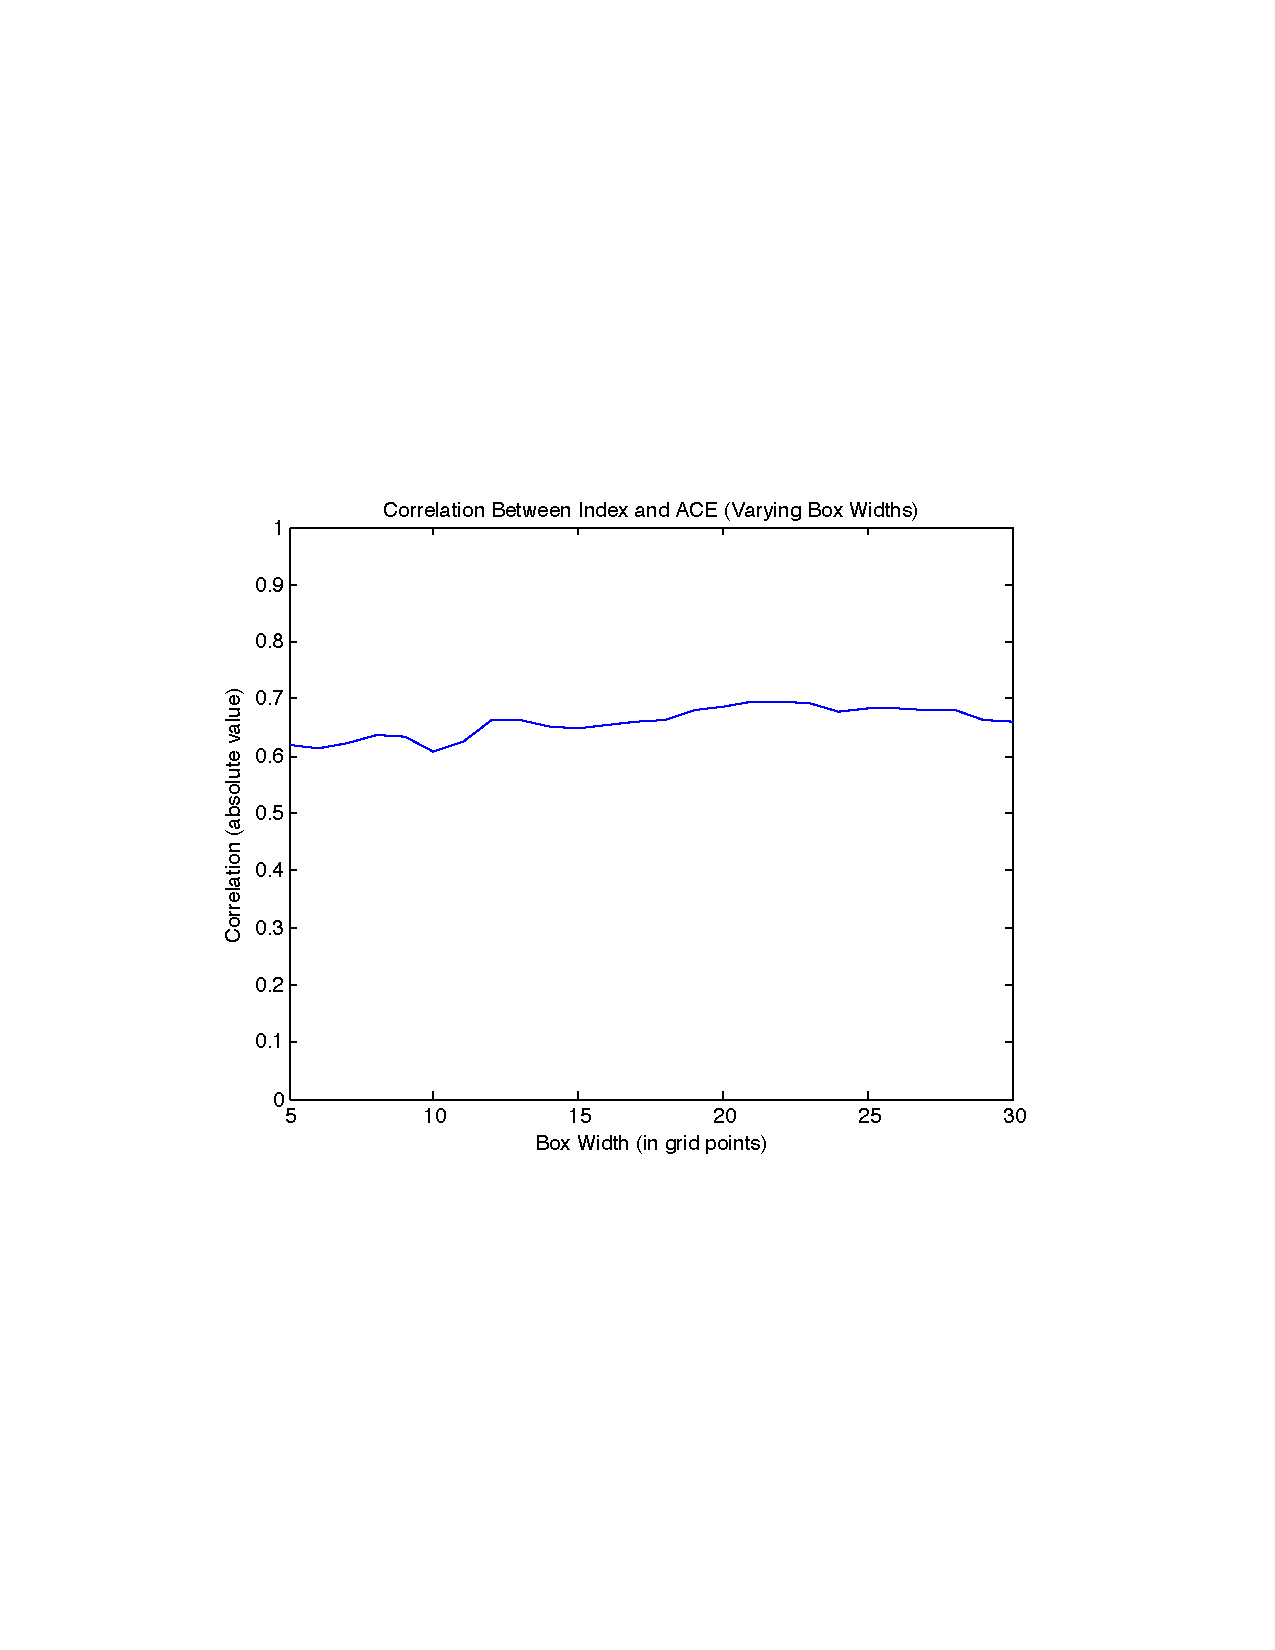
\includegraphics[width=\textwidth]{figs/sensitivityResults/boxSize/ACE_Index_Box_Size.pdf}
\caption{Corr Index vs. ACE}
\label{fig:figure1}
\end{minipage}
\hspace{0cm}
\begin{minipage}[b]{0.6\linewidth}
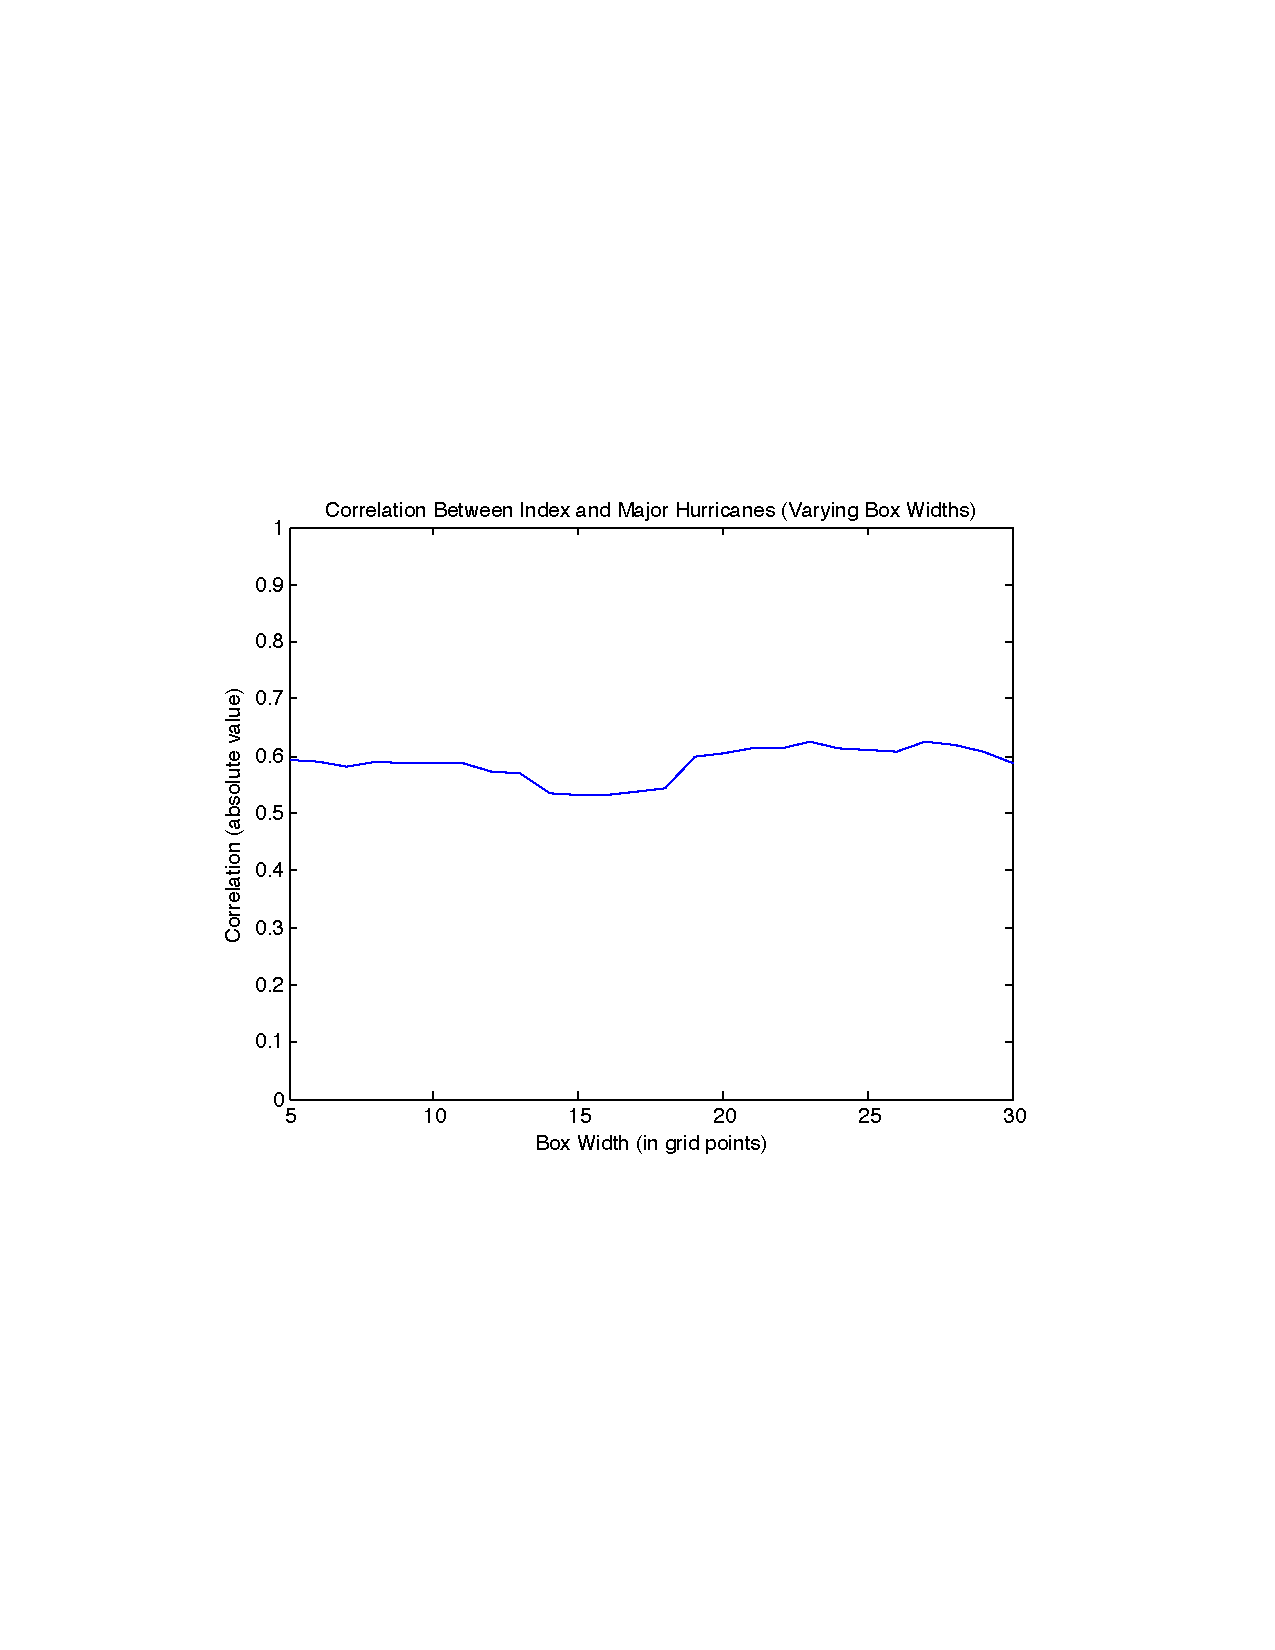
\includegraphics[width=\textwidth]{figs/sensitivityResults/boxSize/Major_Hurricanes_Index_Box_Size.pdf}
\caption{Corr Index vs. Major Hurricanes}
\label{fig:figure2}
\end{minipage}
\end{figure}
\begin{figure}[ht]
\begin{minipage}[b]{0.6\linewidth}
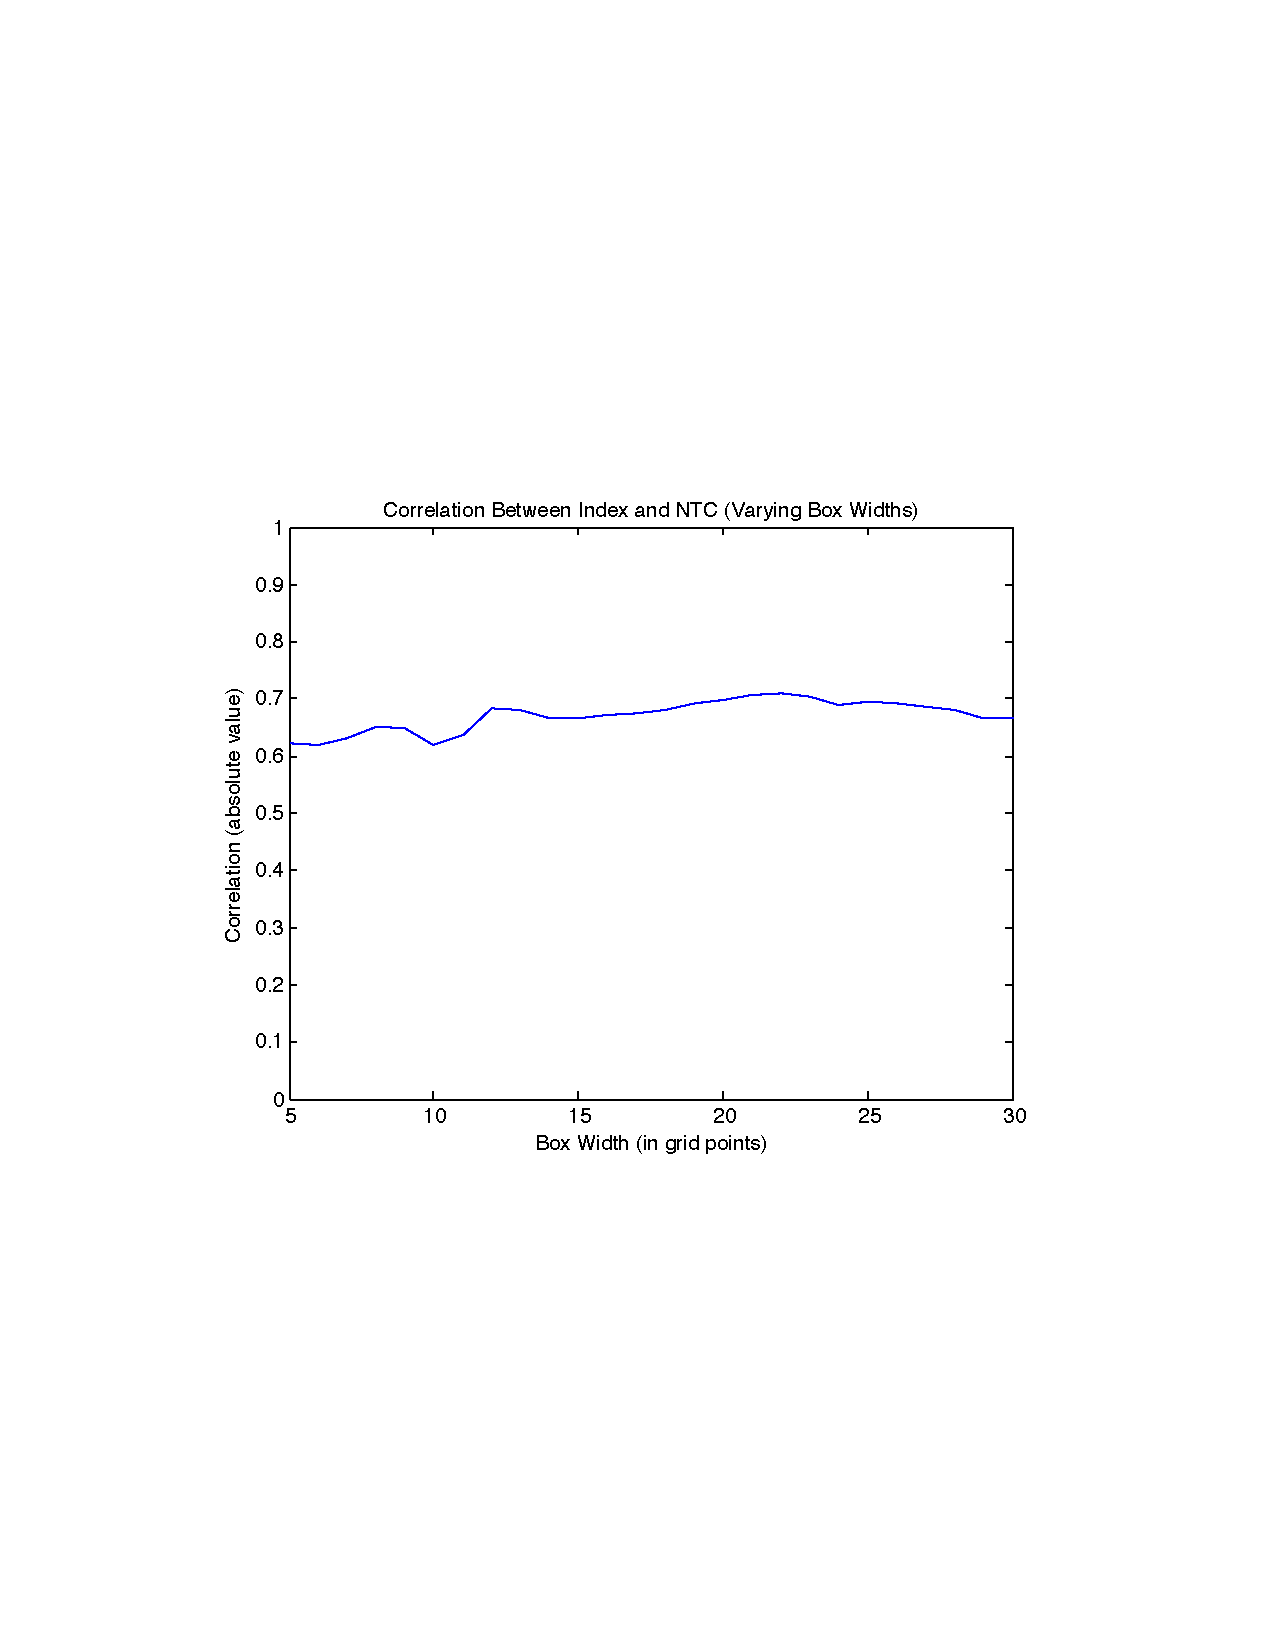
\includegraphics[width=\textwidth]{figs/sensitivityResults/boxSize/NTC_Index_Box_Size.pdf}
\caption{Corr Index vs. NTC}
\label{fig:figure3}
\end{minipage}
\hspace{0cm}
\begin{minipage}[b]{0.6\linewidth}
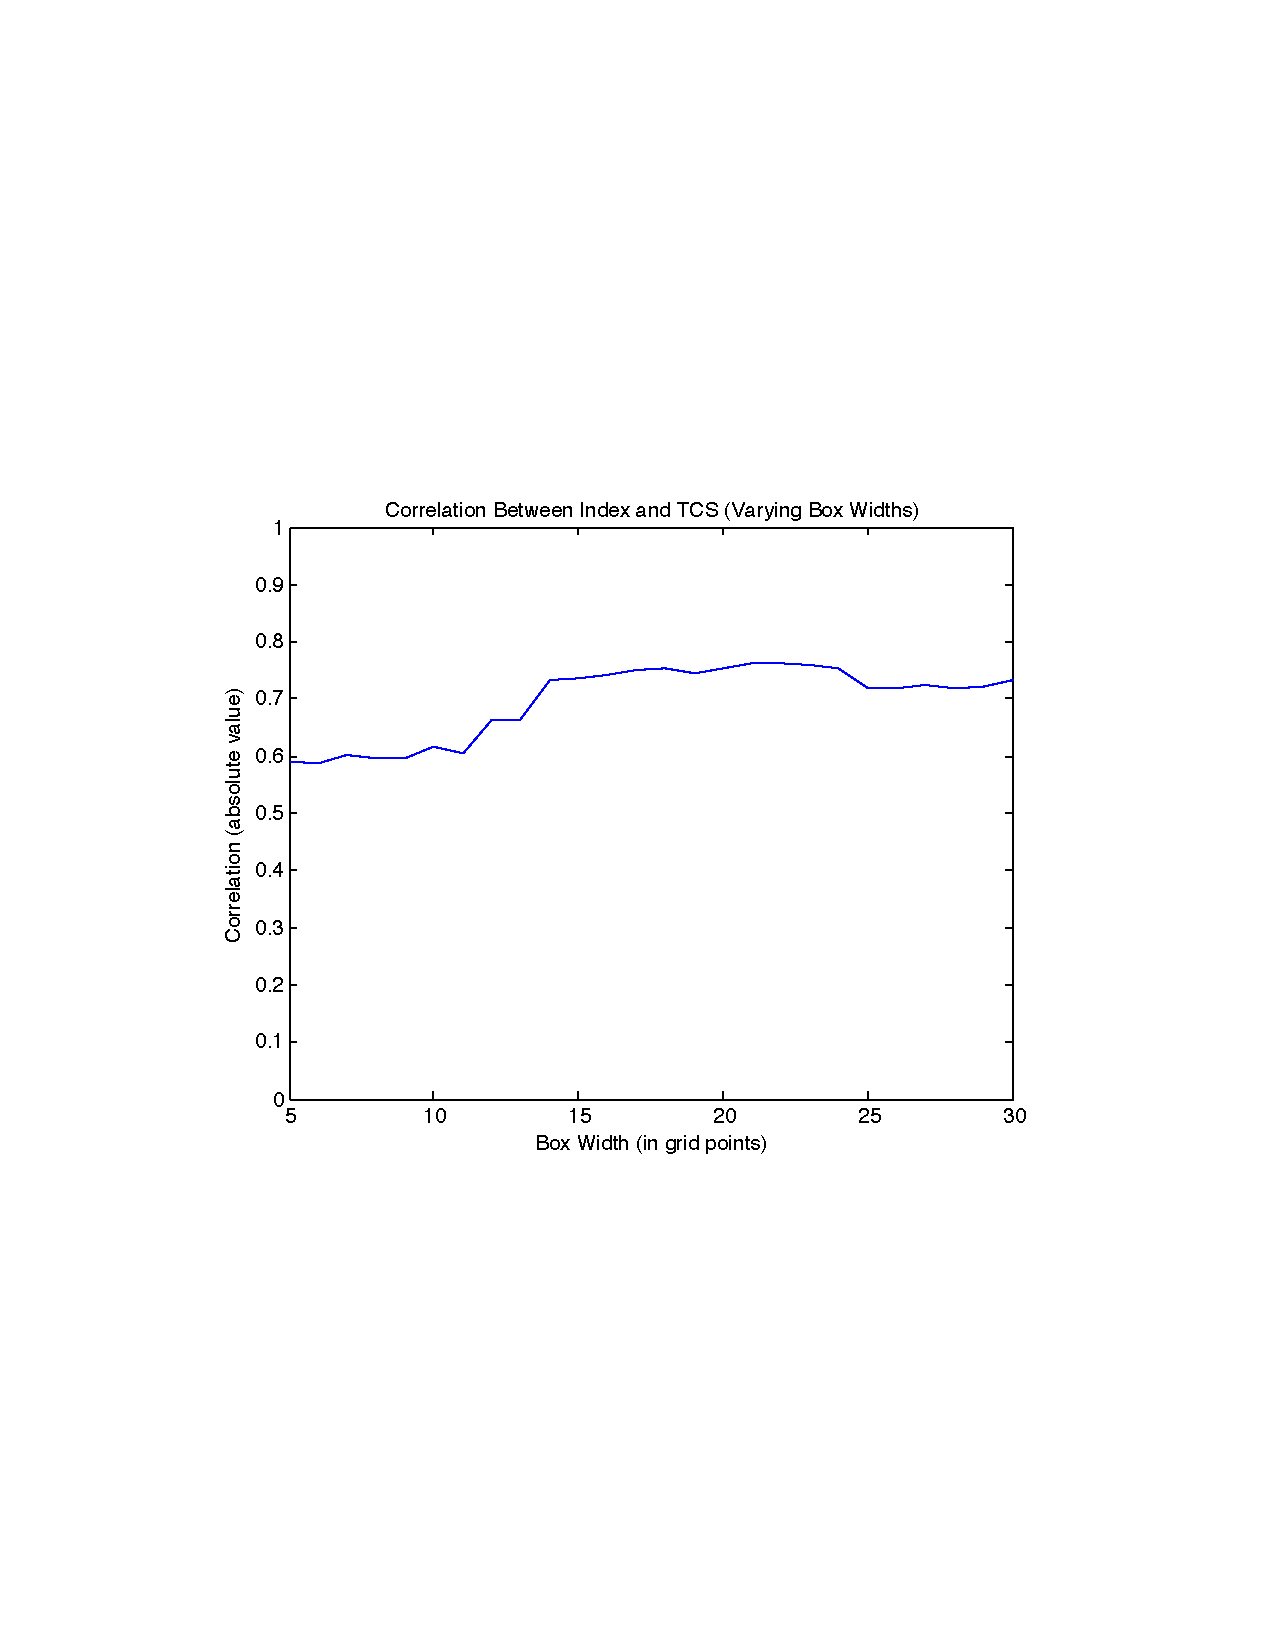
\includegraphics[width=\textwidth]{figs/sensitivityResults/boxSize/TCS_Index_Box_Size.pdf}
\caption{Corr Index vs. TCs}
\label{fig:figure4}
\end{minipage}
\end{figure}
\pagebreak
\subsection{Varying Month Ranges}

\begin{figure}[ht]
\begin{minipage}[b]{0.6\linewidth}
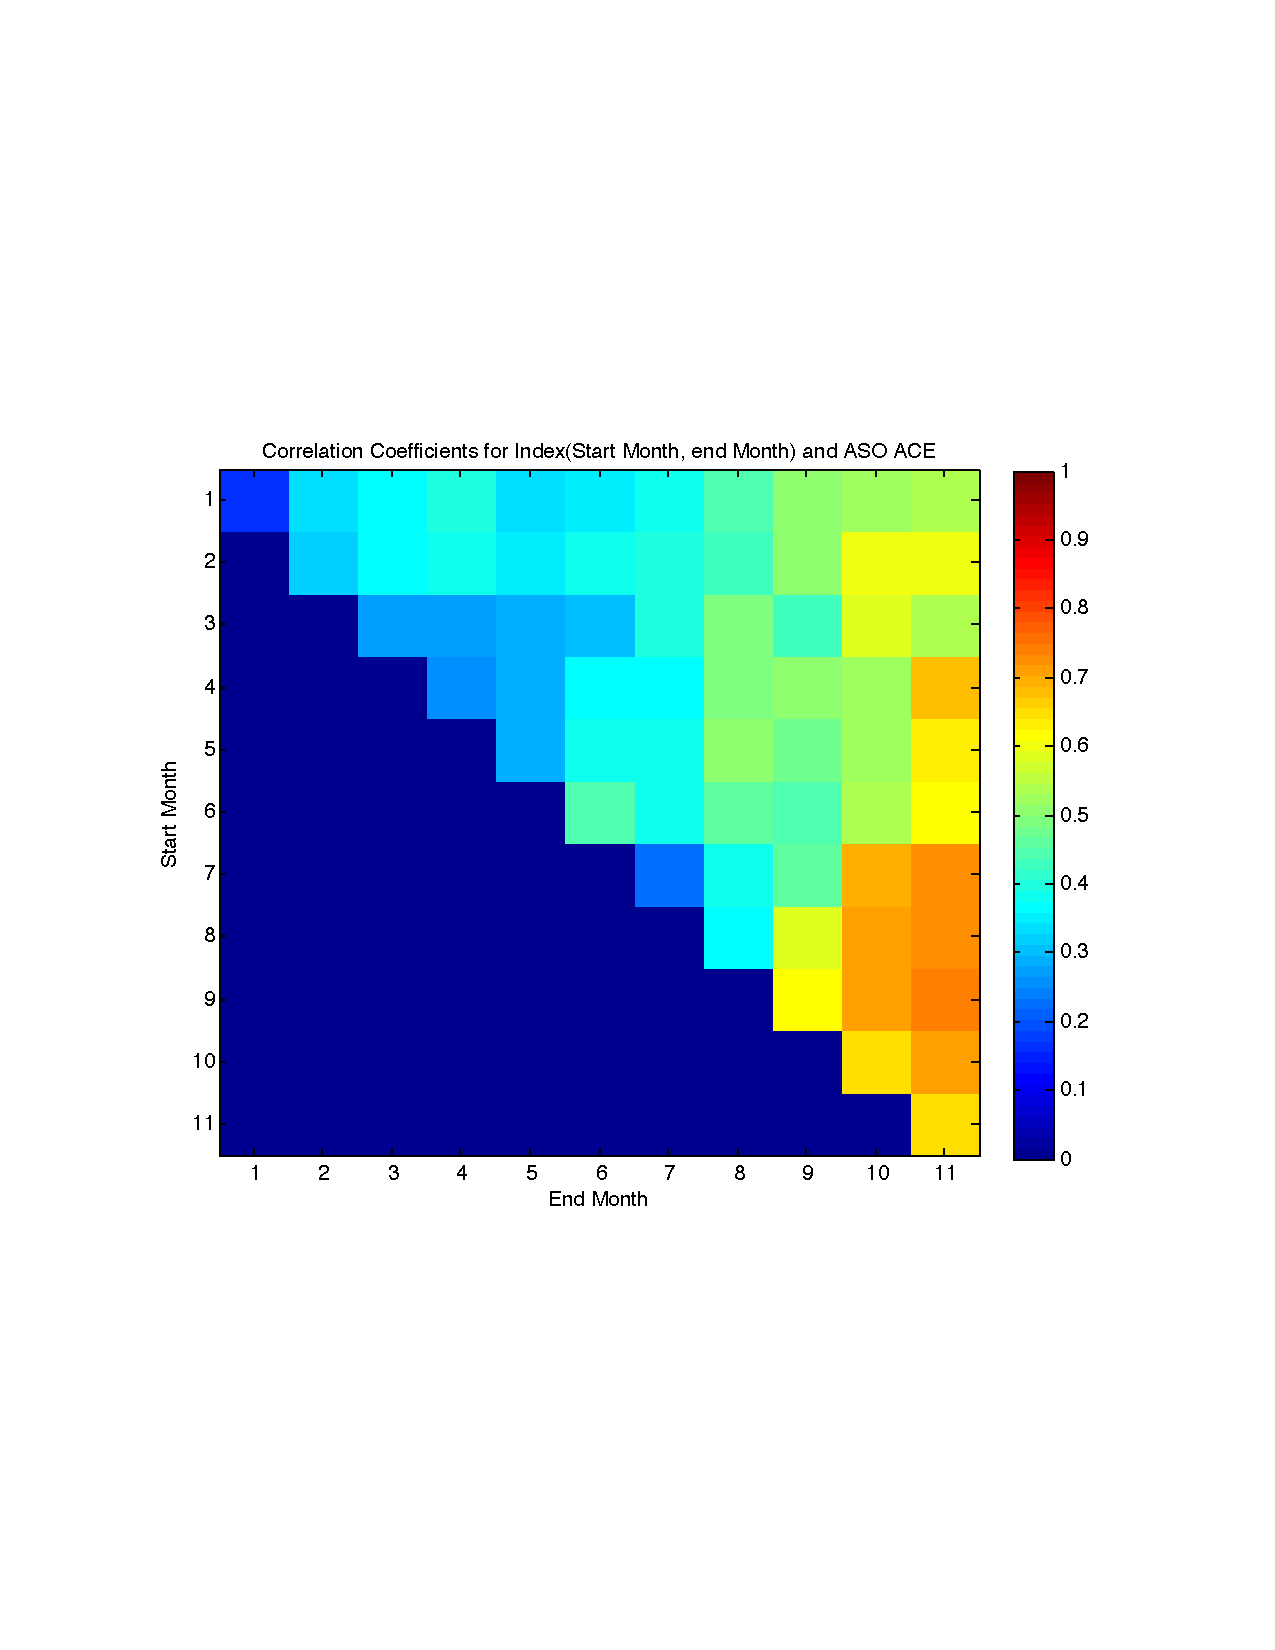
\includegraphics[width=\textwidth]{figs/sensitivityResults/monthRanges/index_corr_month_ranges_ace_month_range.pdf}
\caption{Corr Index vs. ACE}
\label{fig:figure5}
\end{minipage}
\hspace{0cm}
\begin{minipage}[b]{0.6\linewidth}
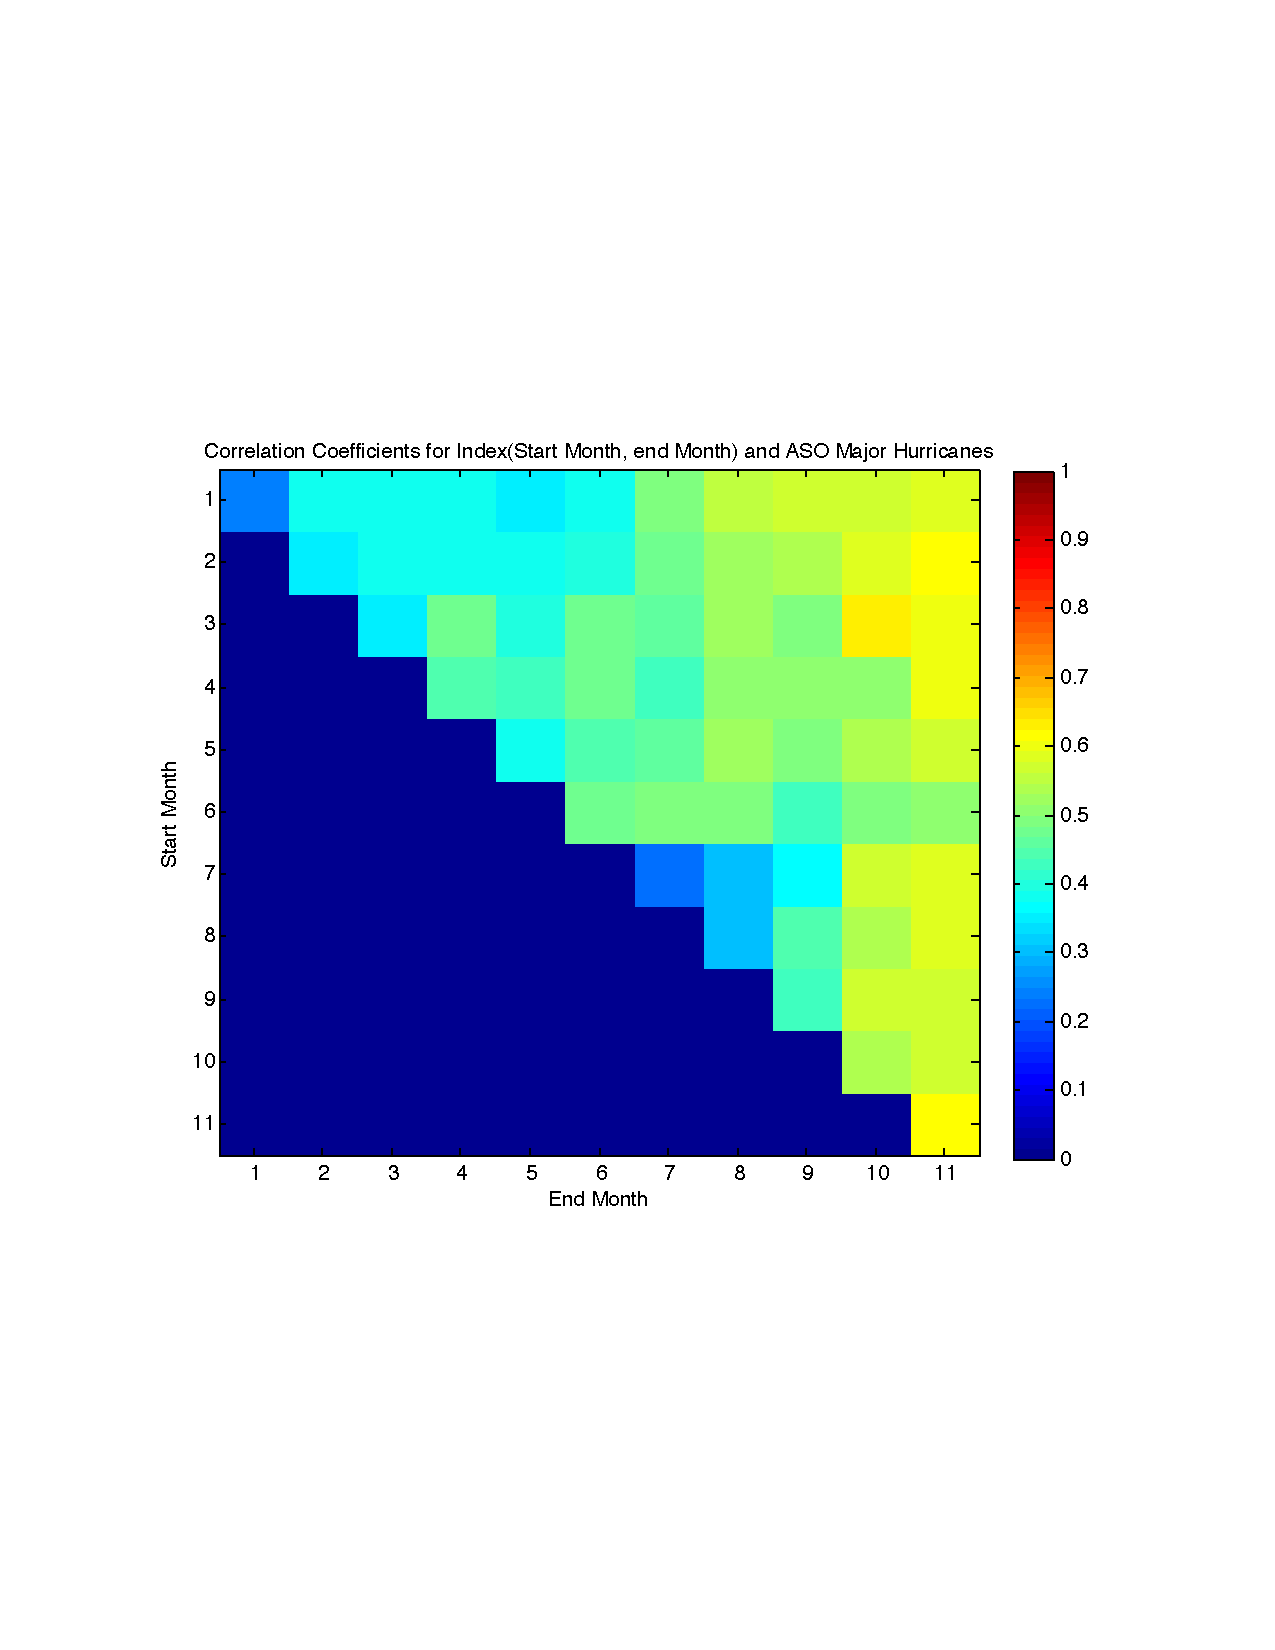
\includegraphics[width=\textwidth]{figs/sensitivityResults/monthRanges/index_corr_month_ranges_hurr_month_range.pdf}
\caption{Corr Index vs. Major Hurricanes}
\label{fig:figure6}
\end{minipage}
\end{figure}

\begin{figure}[ht]
\begin{minipage}[b]{0.6\linewidth}
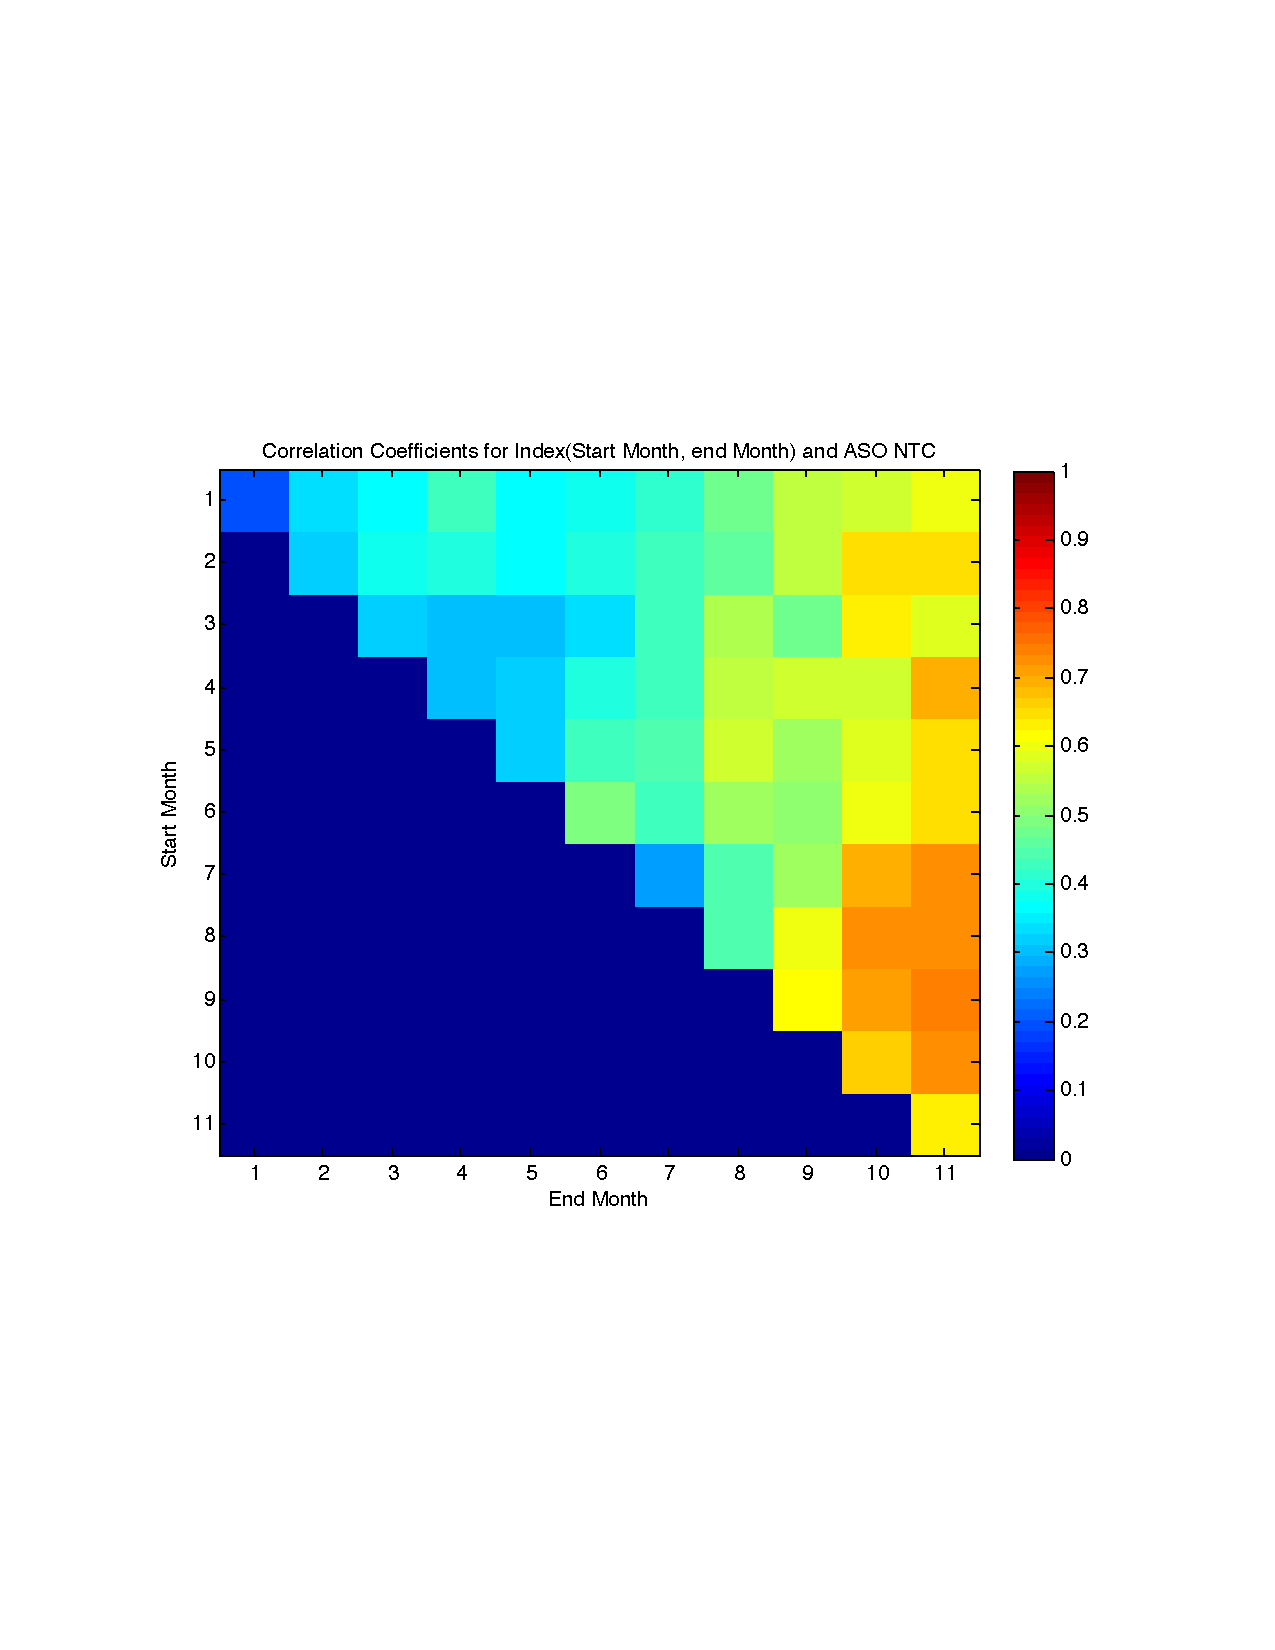
\includegraphics[width=\textwidth]{figs/sensitivityResults/monthRanges/index_corr_month_ranges_ntc_month_range.pdf}
\caption{Corr Index vs. NTC}
\label{fig:figure7}
\end{minipage}
\hspace{0cm}
\begin{minipage}[b]{0.6\linewidth}
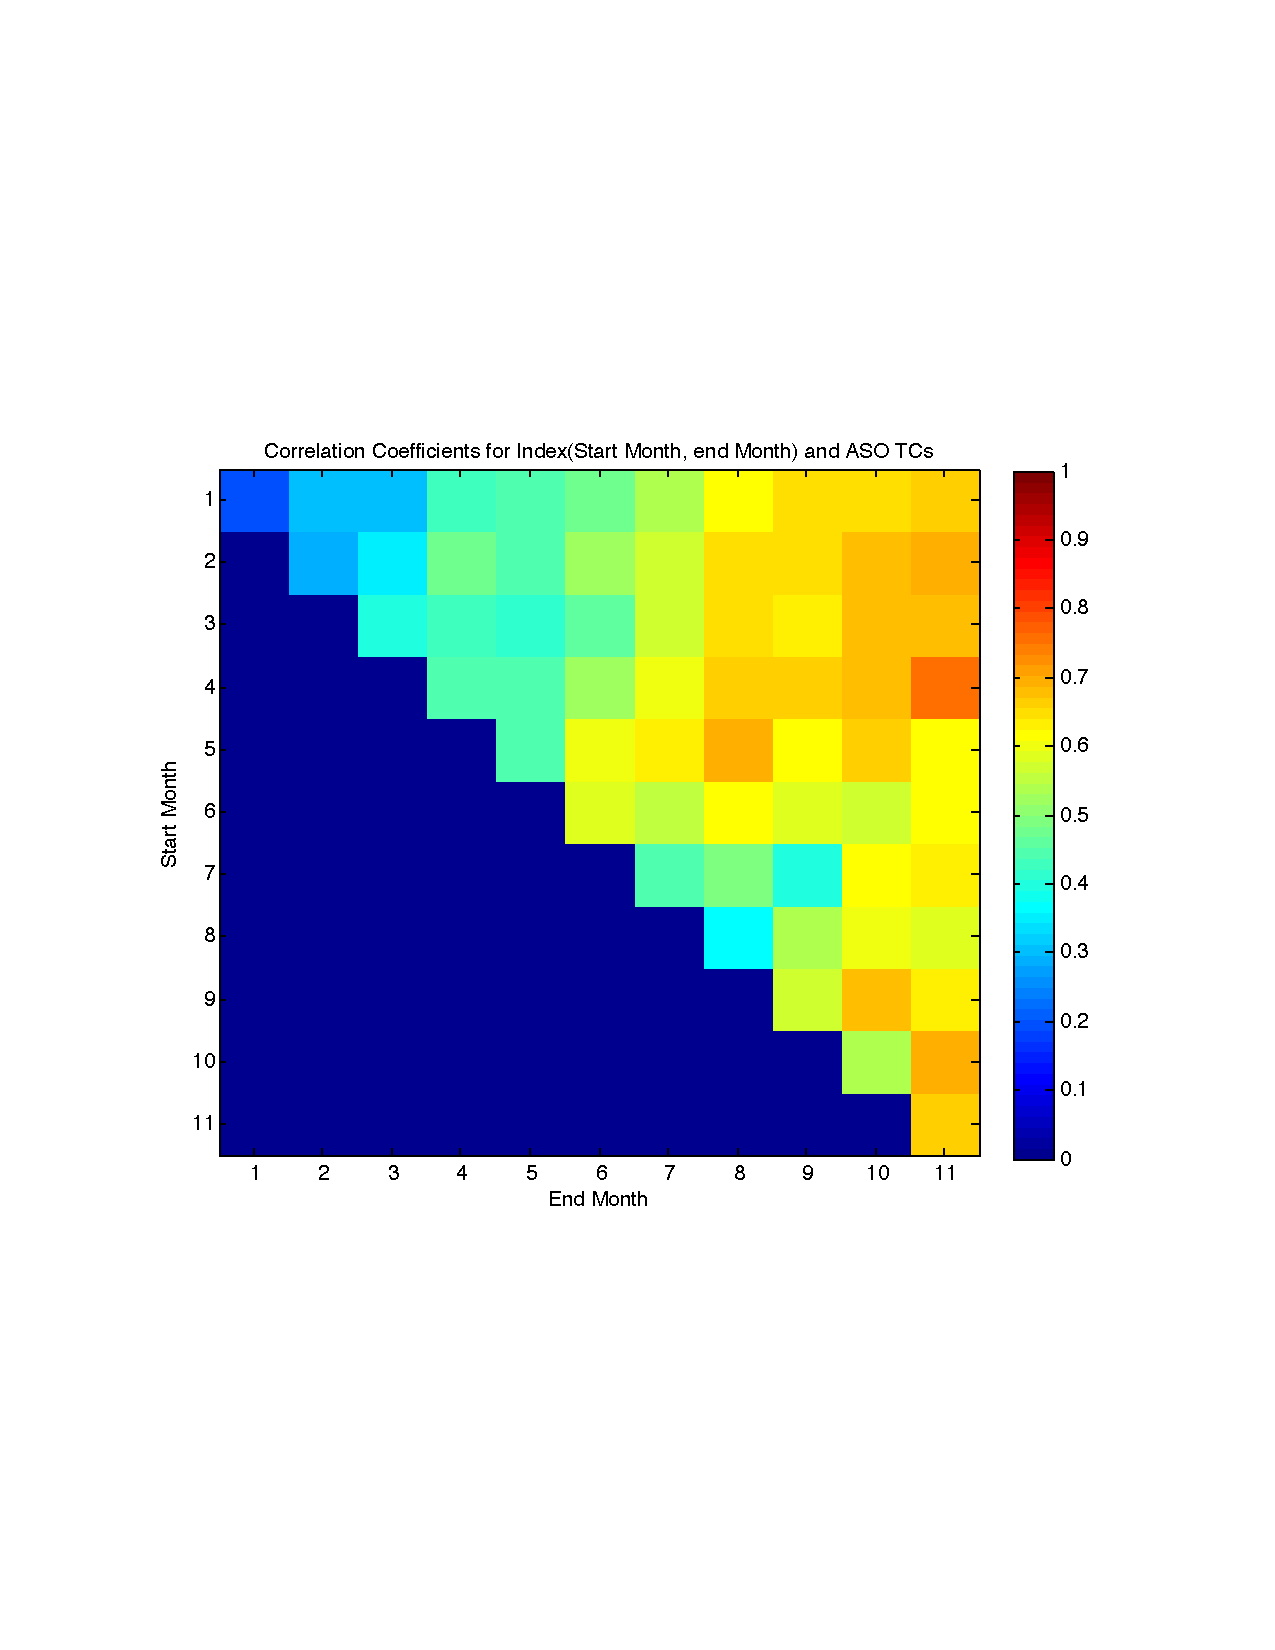
\includegraphics[width=\textwidth]{figs/sensitivityResults/monthRanges/index_corr_month_ranges_tcs_month_range.pdf}
\caption{Corr Index vs. TCs}
\label{fig:figure8}
\end{minipage}
\end{figure}

\pagebreak
\subsection{Varying Search Space (North and South Hemispheres)}
\begin{figure}[ht]
\begin{minipage}[b]{0.6\linewidth}
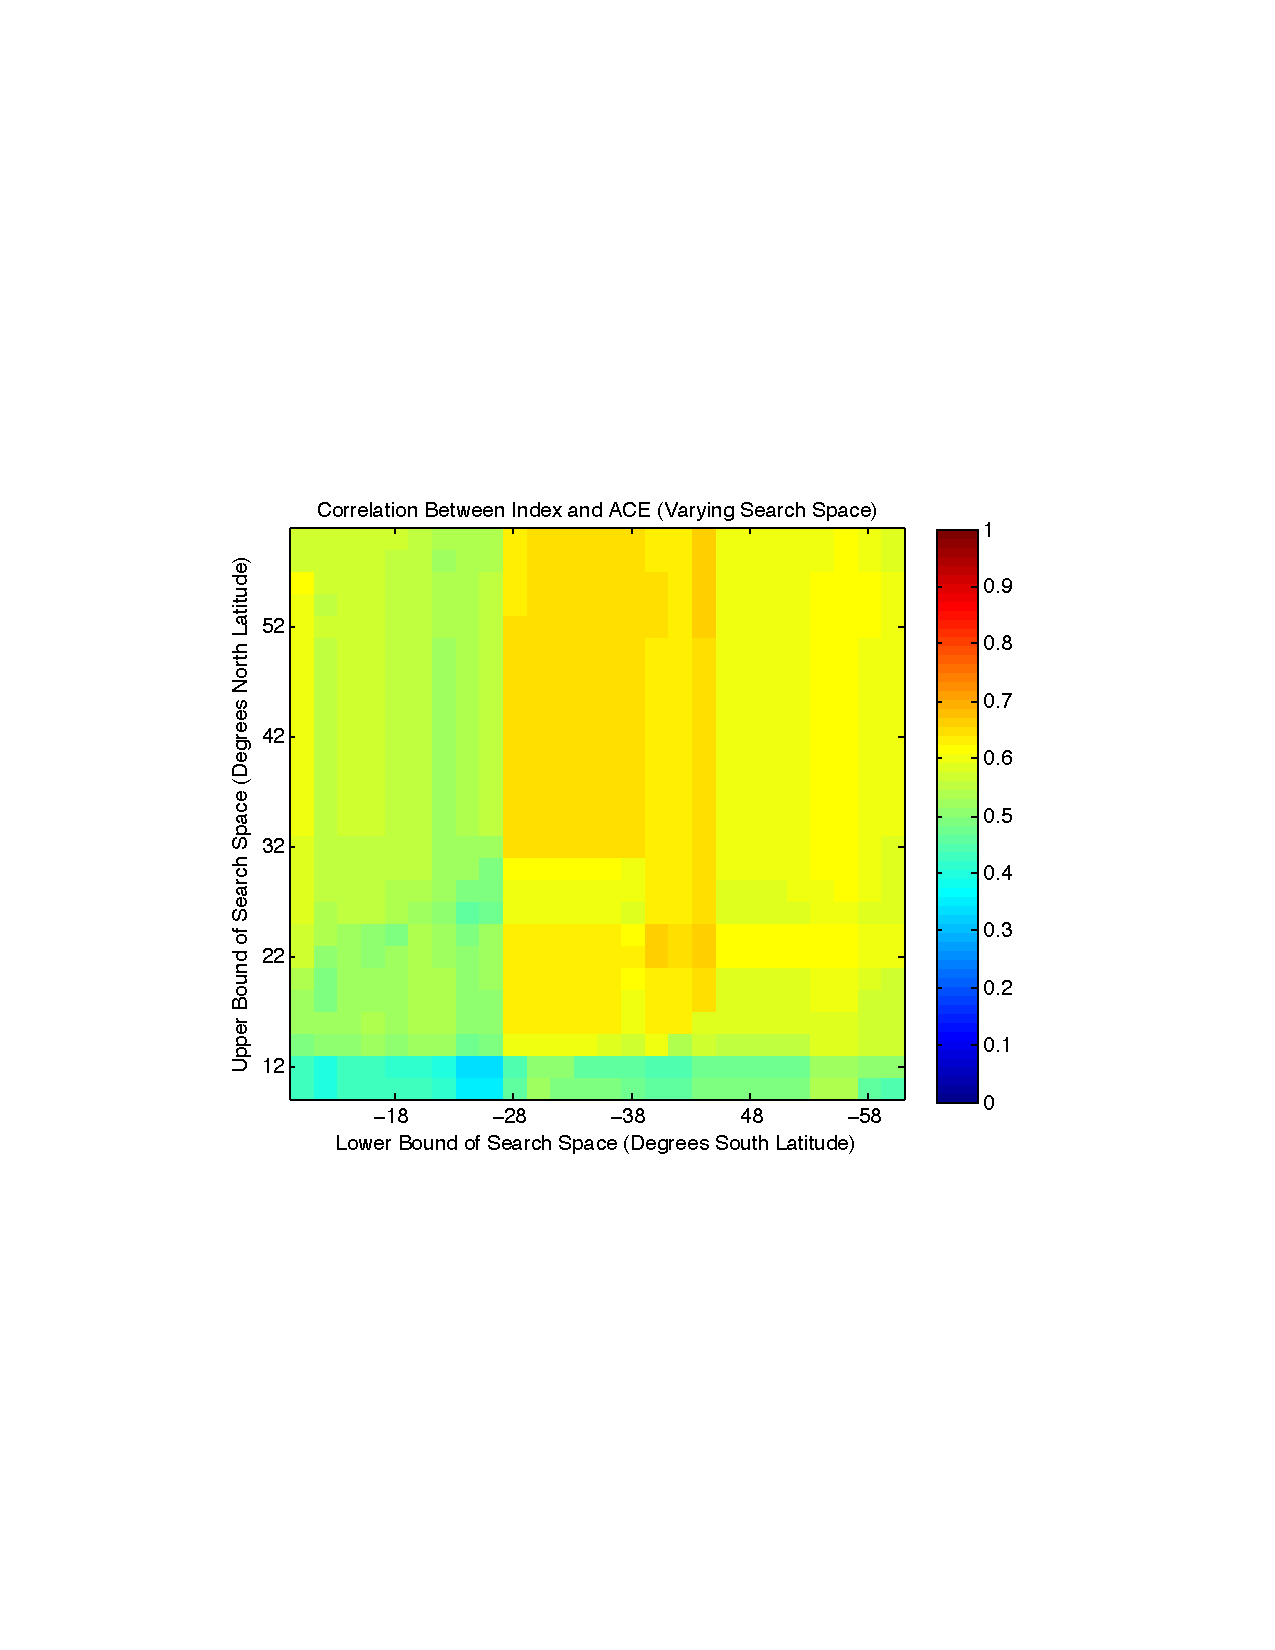
\includegraphics[width=\textwidth]{figs/sensitivityResults/northSouthHem/ACE_Index_North_South.pdf}
\caption{Corr Index vs. ACE}
\label{fig:figure9}
\end{minipage}
\hspace{0cm}
\begin{minipage}[b]{0.6\linewidth}
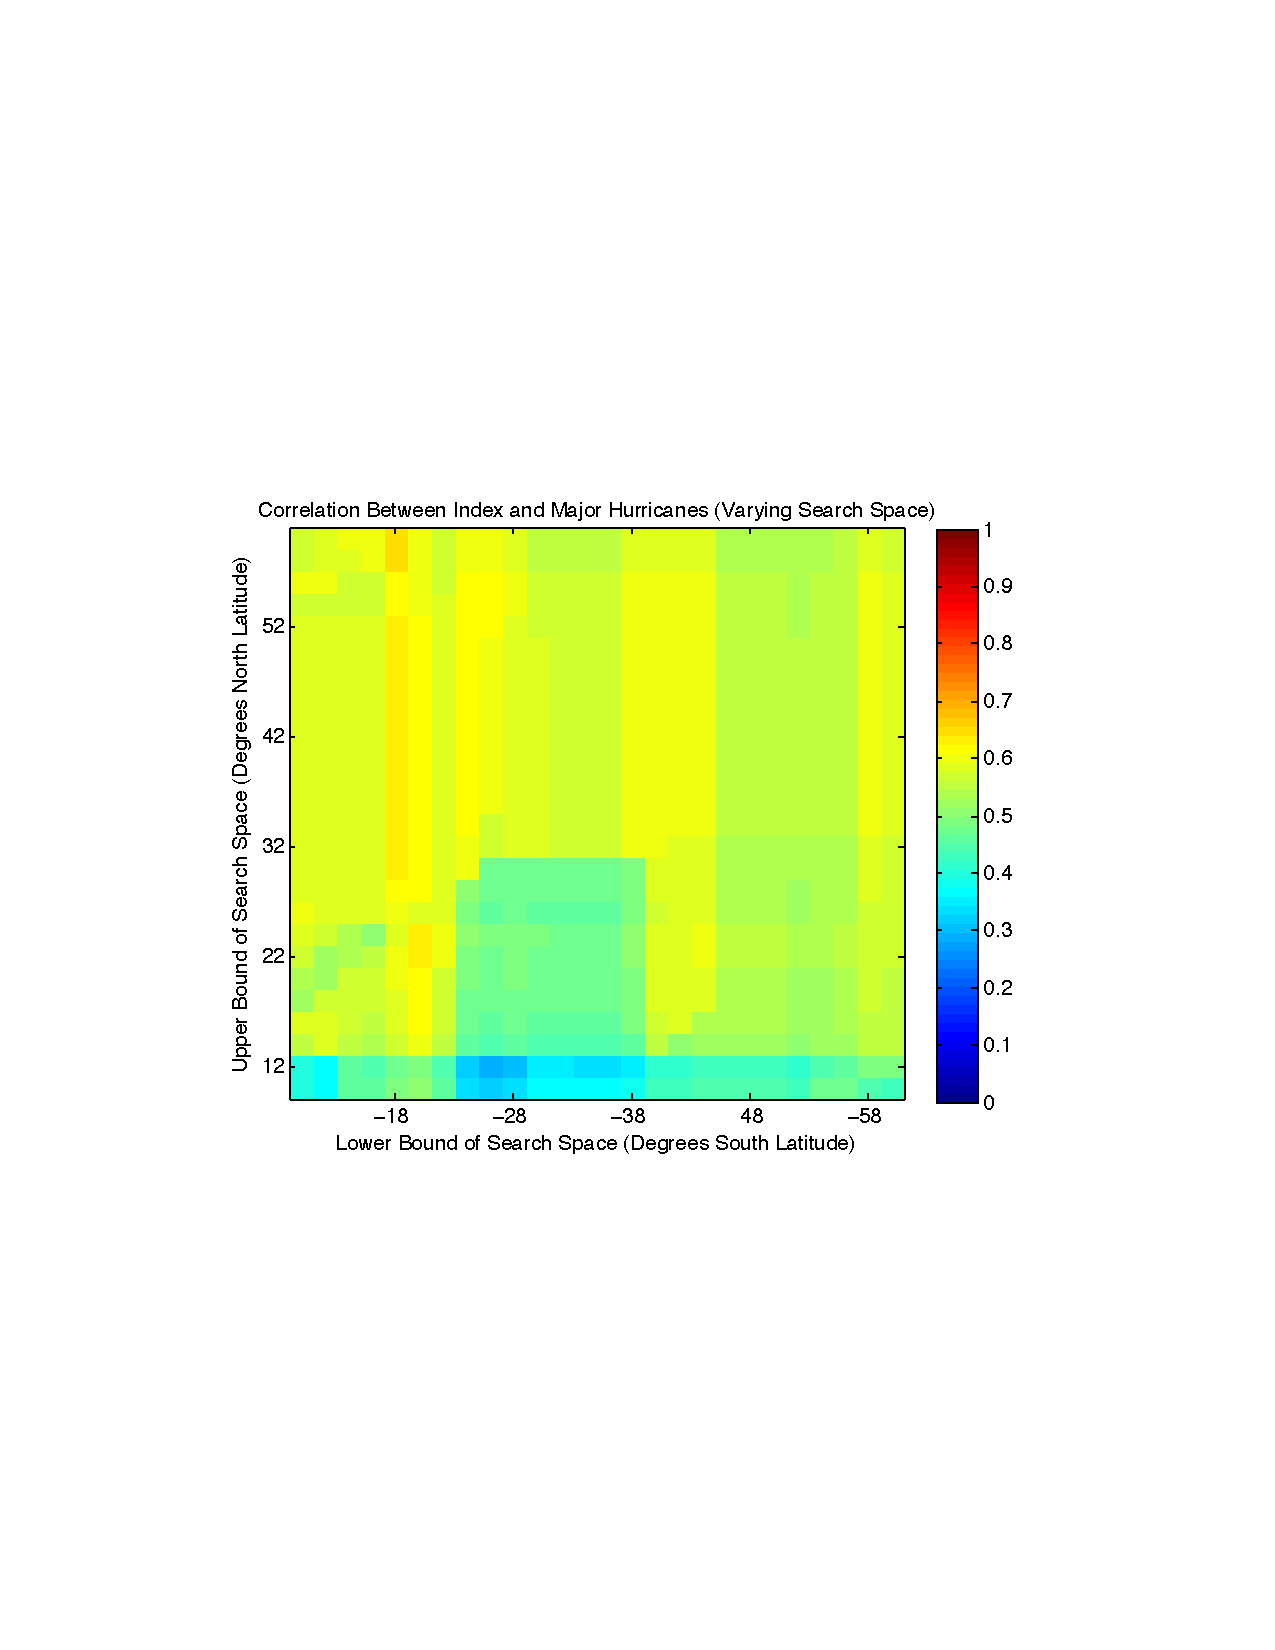
\includegraphics[width=\textwidth]{figs/sensitivityResults/northSouthHem/Major_Hurricanes_Index_North_South.pdf}
\caption{Corr Index vs. Major Hurricanes}
\label{fig:figure10}
\end{minipage}
\end{figure}

\begin{figure}[ht]
\begin{minipage}[b]{0.6\linewidth}
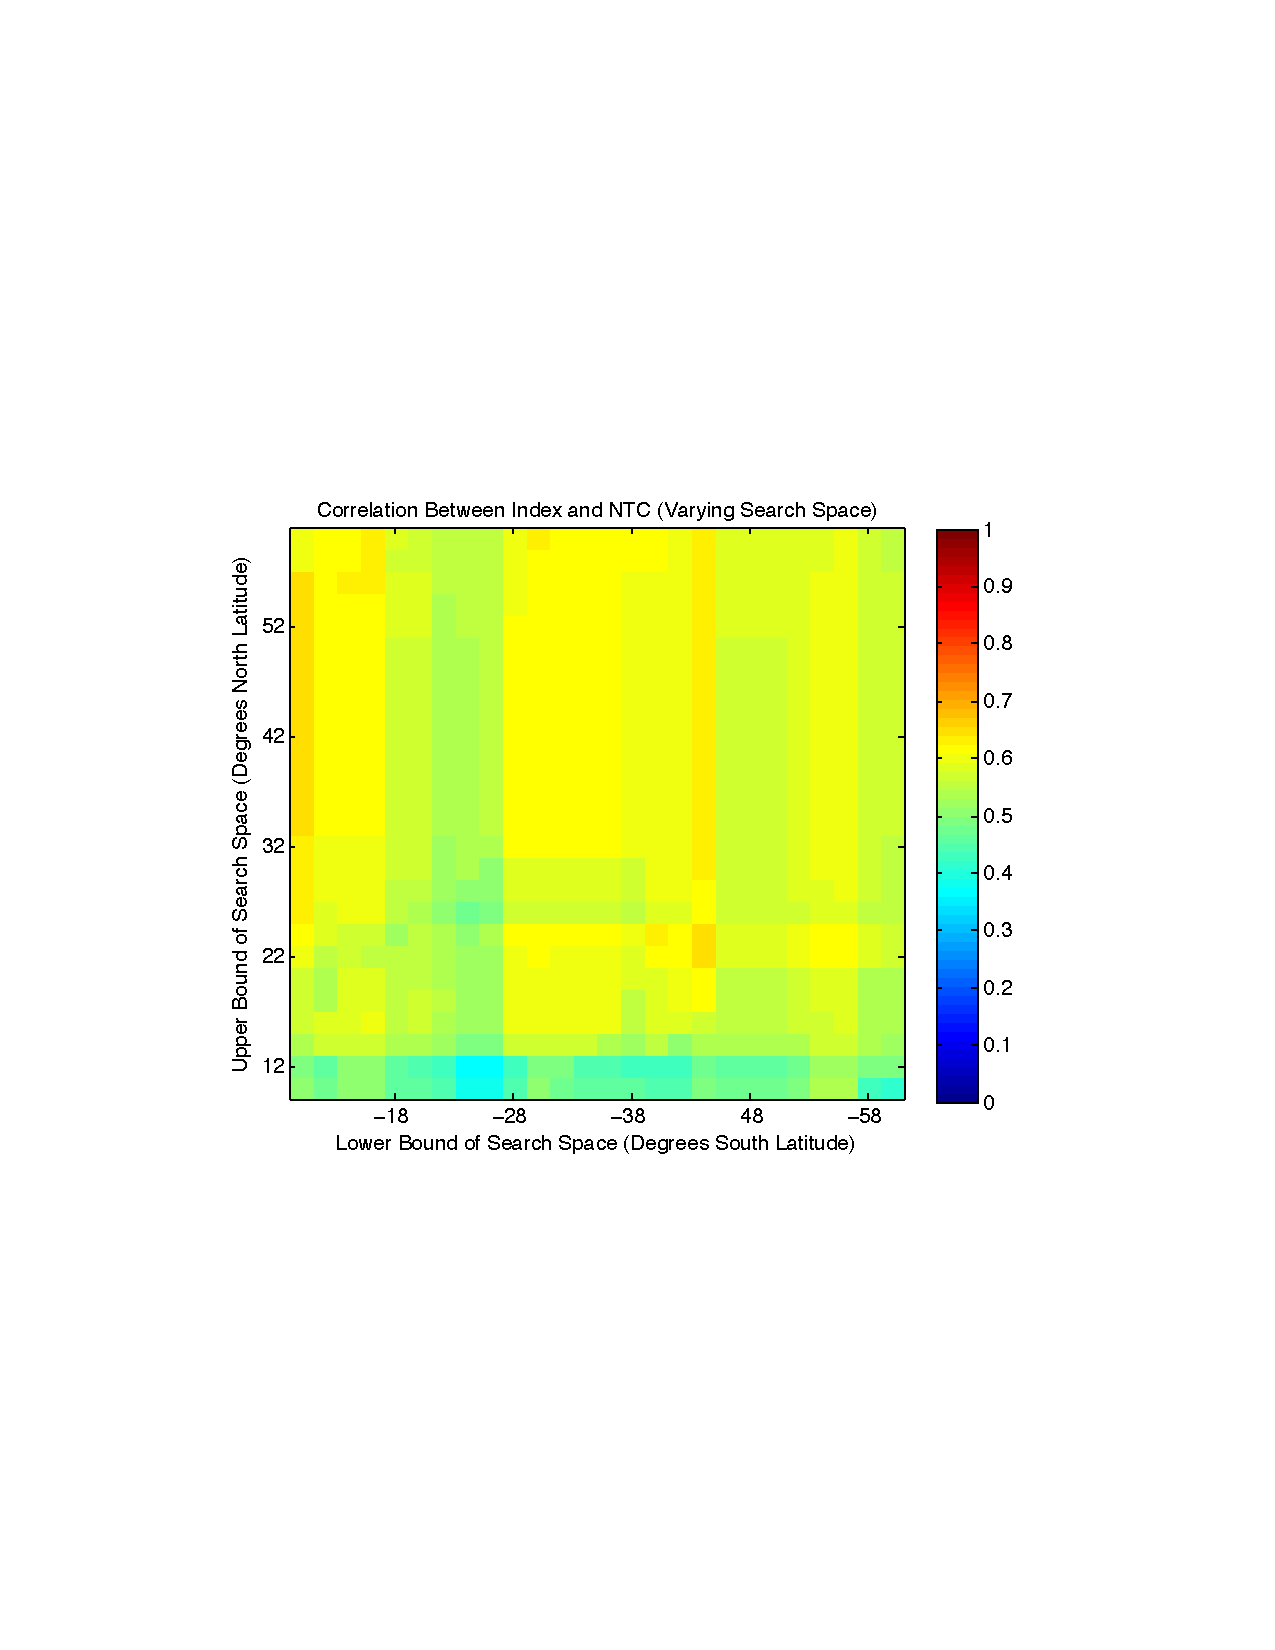
\includegraphics[width=\textwidth]{figs/sensitivityResults/northSouthHem/NTC_Index_North_South.pdf}
\caption{Corr Index vs. NTC}
\label{fig:figure11}
\end{minipage}
\hspace{0cm}
\begin{minipage}[b]{0.6\linewidth}
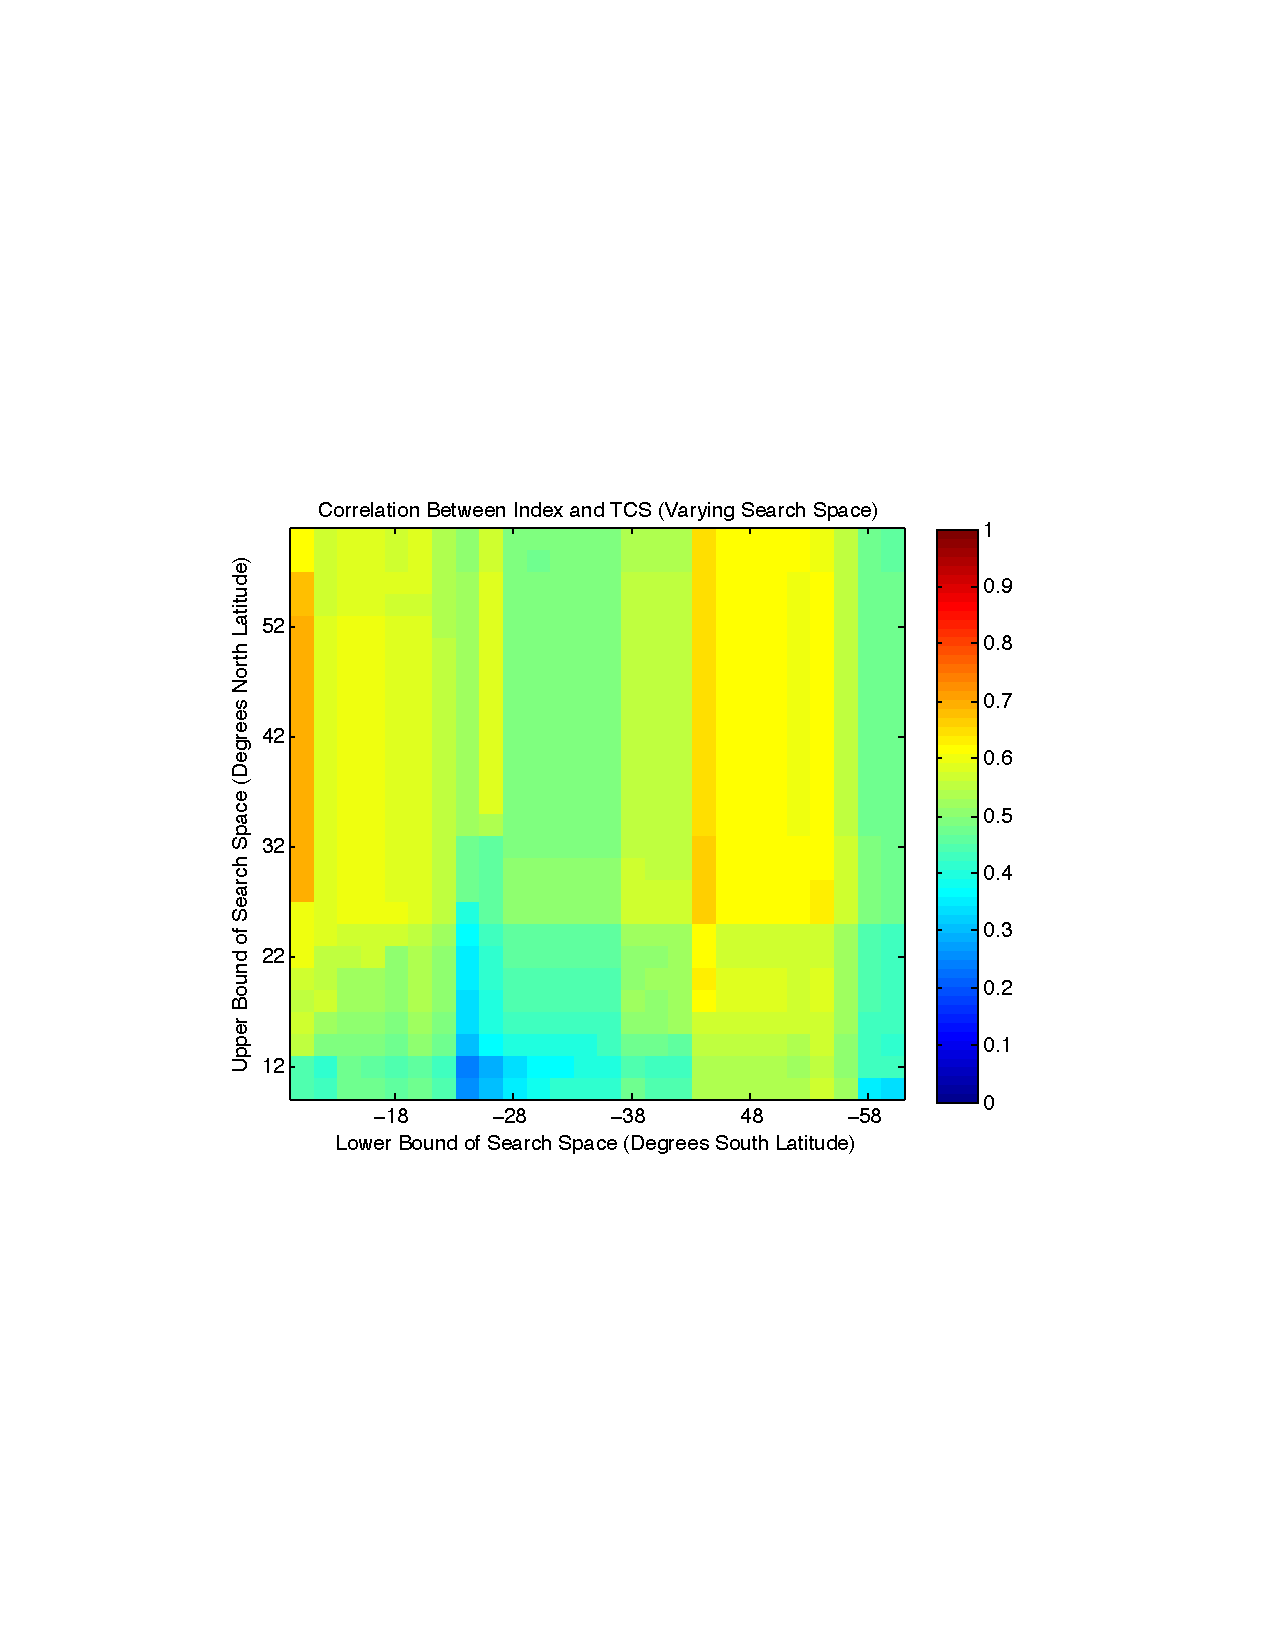
\includegraphics[width=\textwidth]{figs/sensitivityResults/northSouthHem/TCS_Index_North_South.pdf}
\caption{Corr Index vs. TCs}
\label{fig:figure12}
\end{minipage}
\end{figure}
\pagebreak

\subsection{Varying Search Space (North Hemisphere)}

\begin{figure}[ht]
\begin{minipage}[b]{0.6\linewidth}
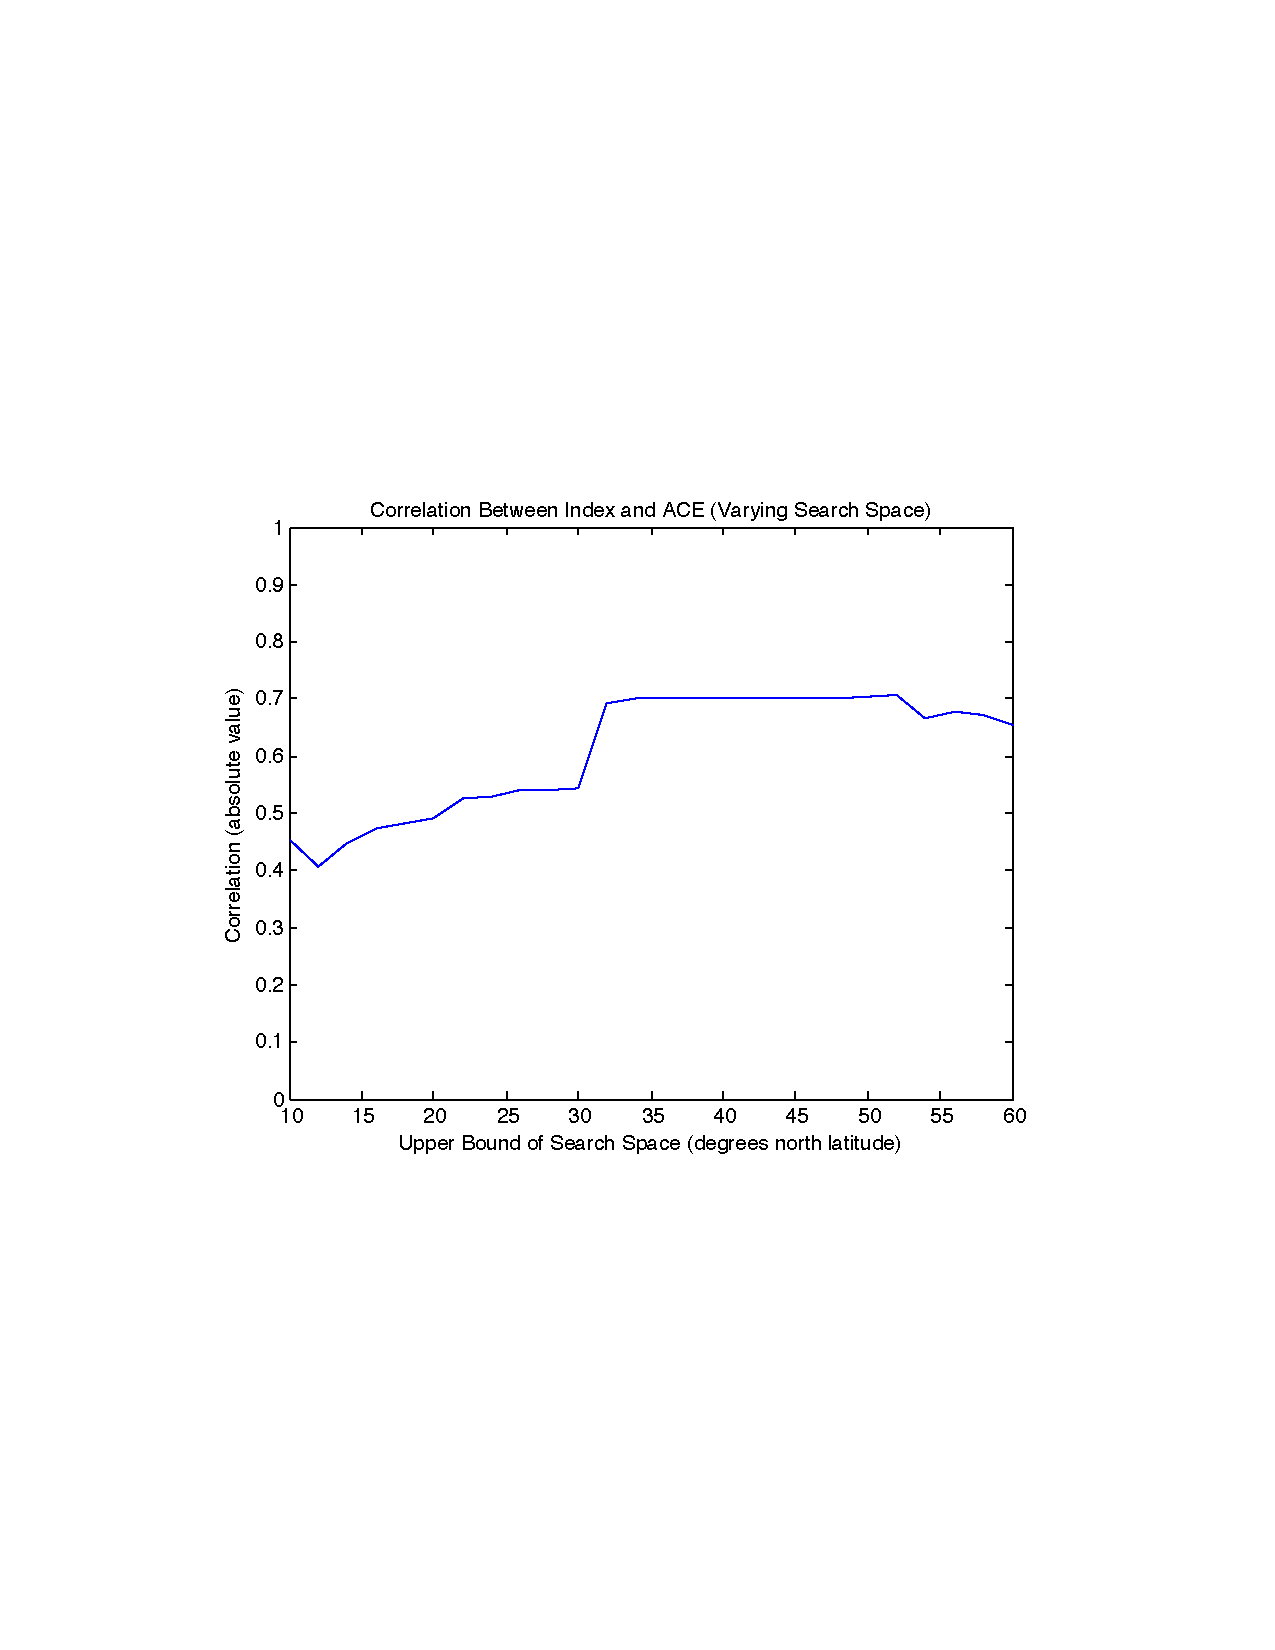
\includegraphics[width=\textwidth]{figs/sensitivityResults/northHem/ACE_Index_North.pdf}
\caption{Corr Index vs. ACE}
\label{fig:figure13}
\end{minipage}
\hspace{0cm}
\begin{minipage}[b]{0.6\linewidth}
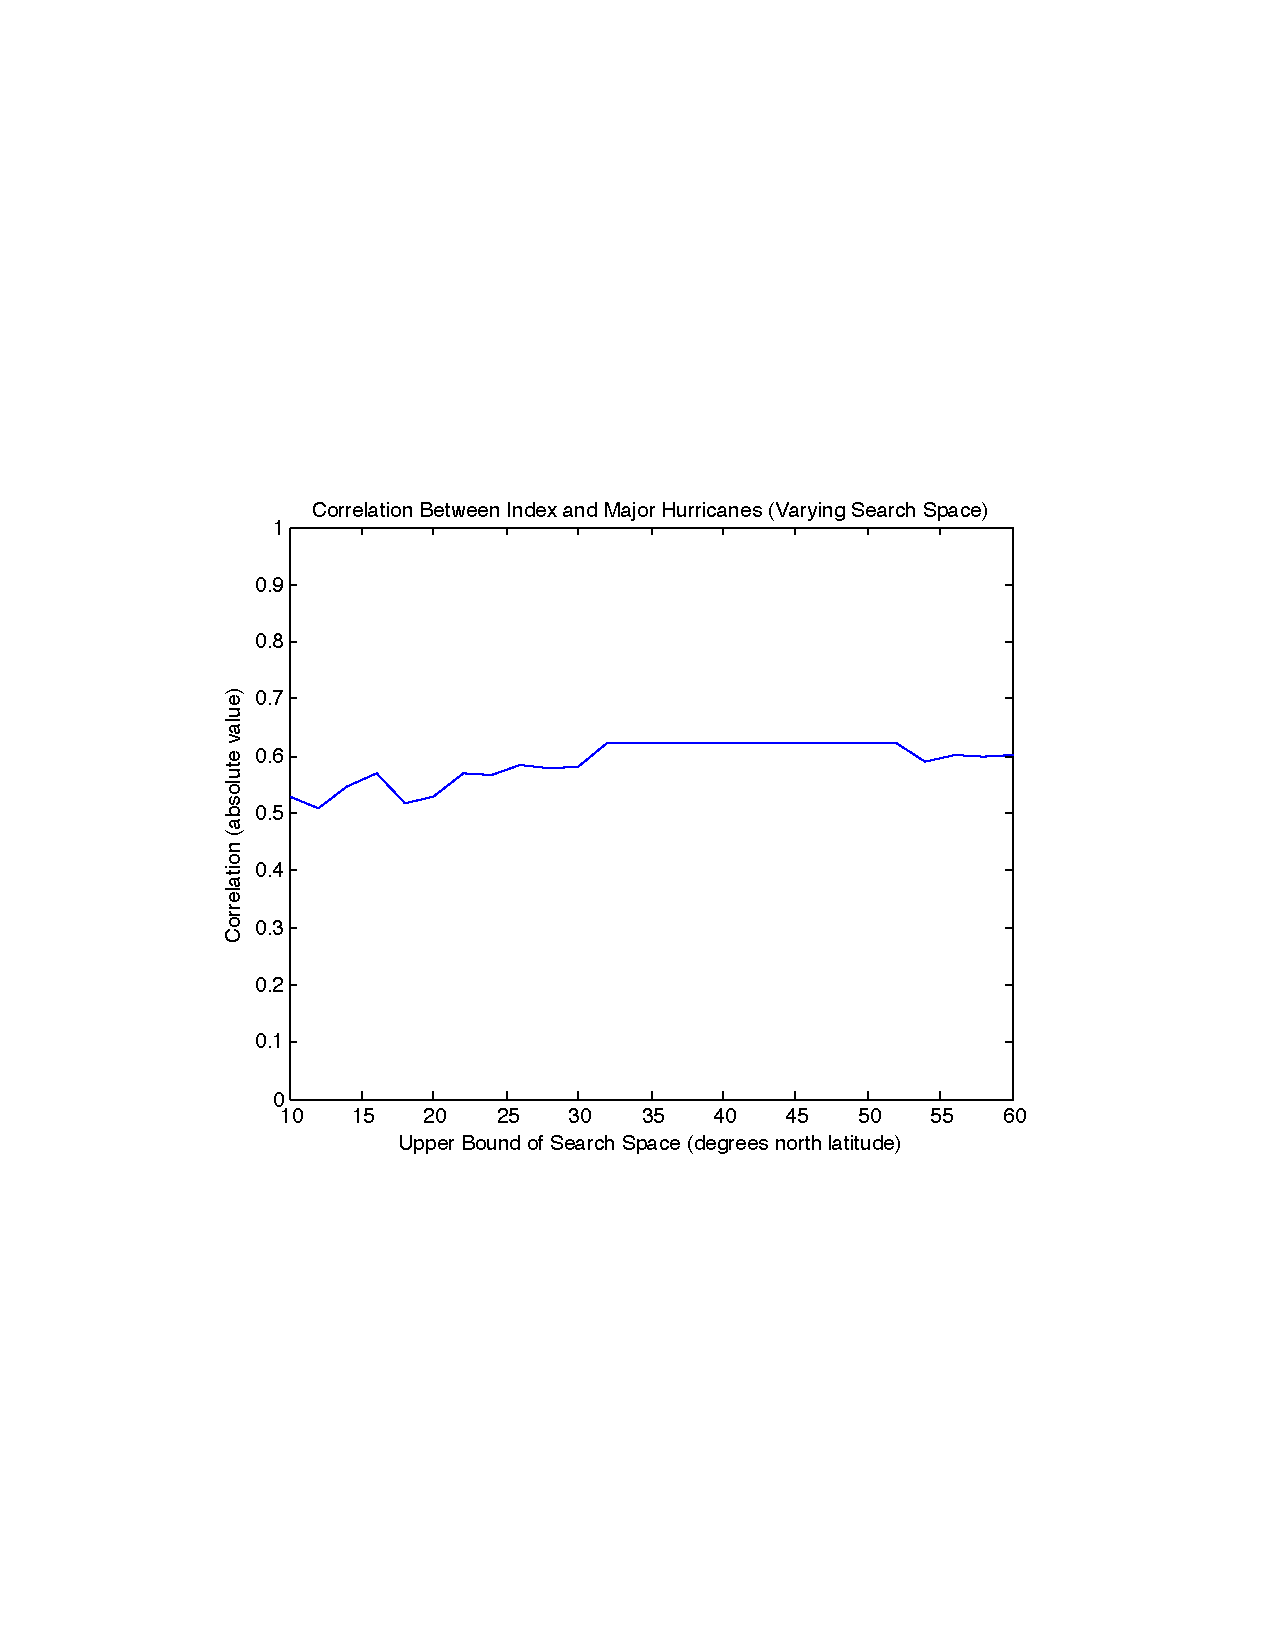
\includegraphics[width=\textwidth]{figs/sensitivityResults/northHem/Major_Hurricanes_Index_North.pdf}
\caption{Corr Index vs. Major Hurricanes}
\label{fig:figure14}
\end{minipage}
\end{figure}

\begin{figure}[ht]
\begin{minipage}[b]{0.6\linewidth}
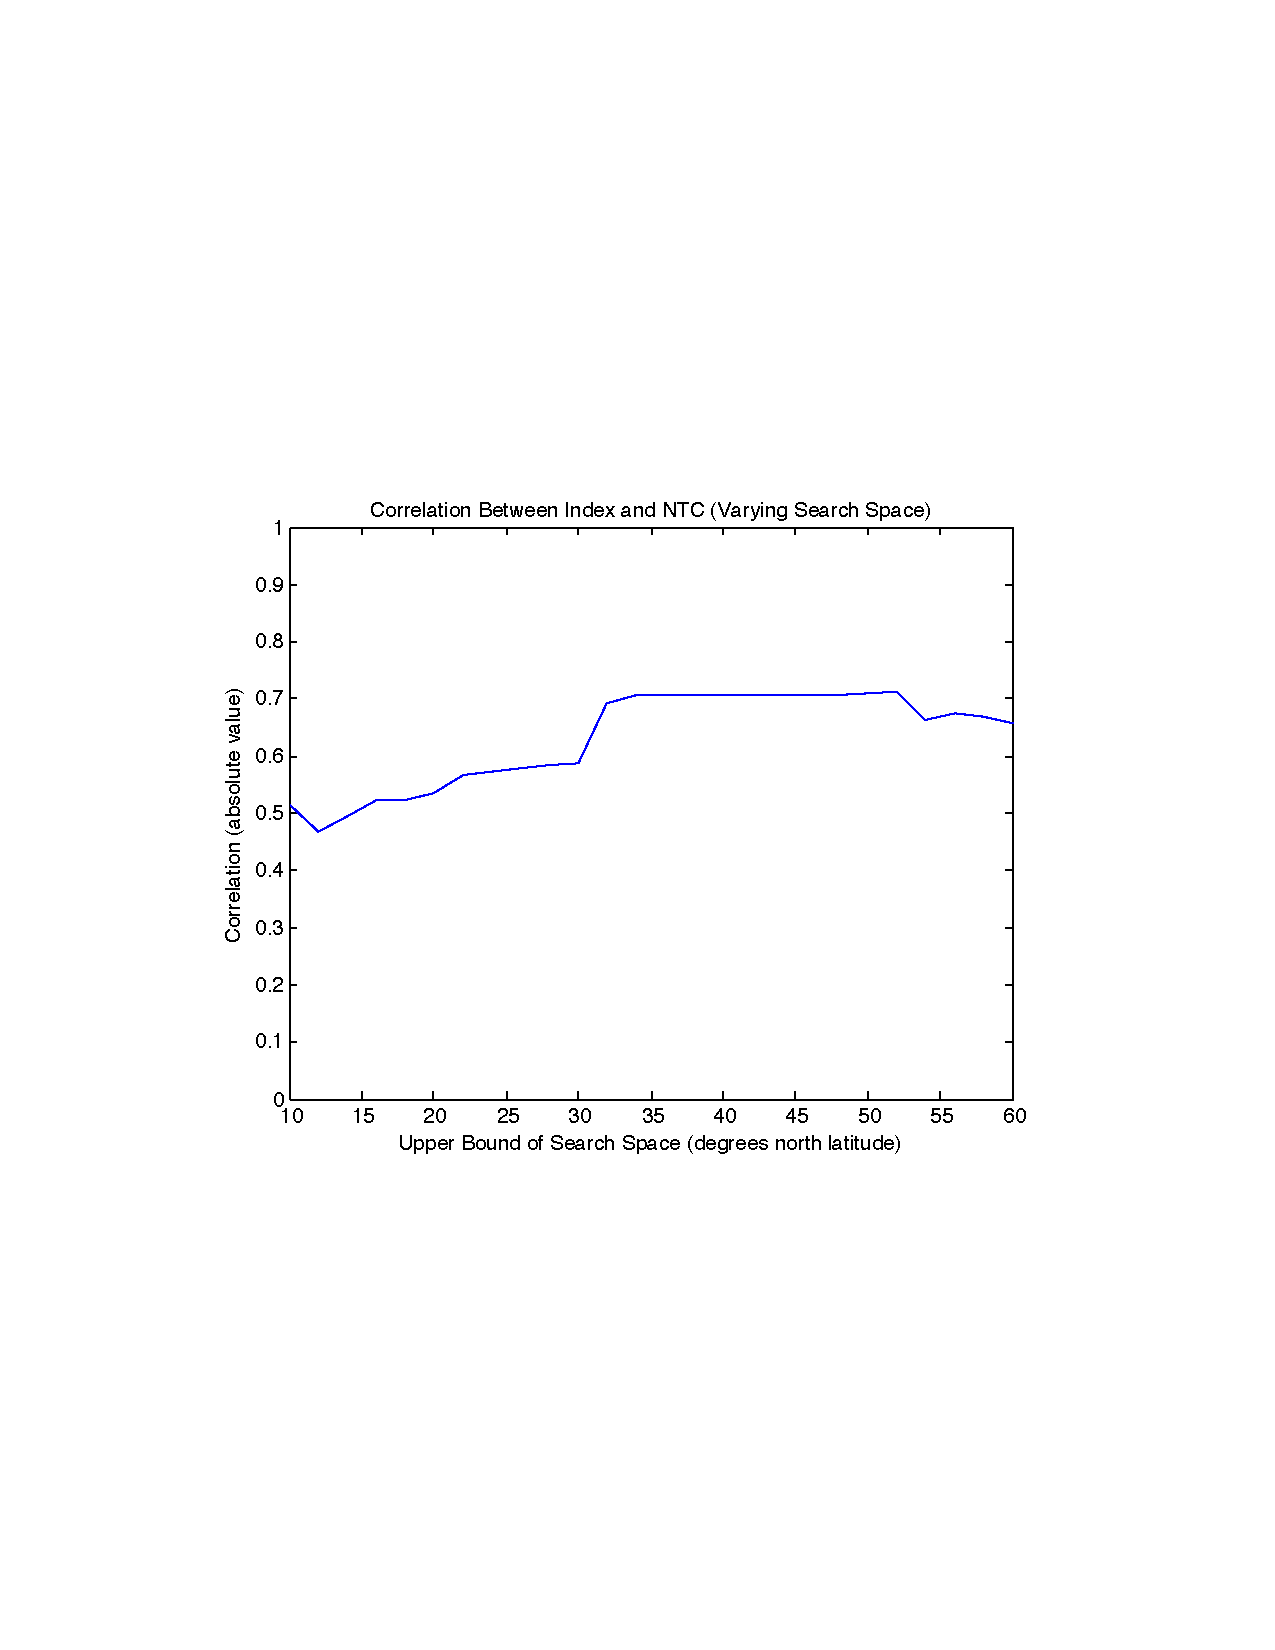
\includegraphics[width=\textwidth]{figs/sensitivityResults/northHem/NTC_Index_North.pdf}
\caption{Corr Index vs. NTC}
\label{fig:figure15}
\end{minipage}
\hspace{0cm}
\begin{minipage}[b]{0.6\linewidth}
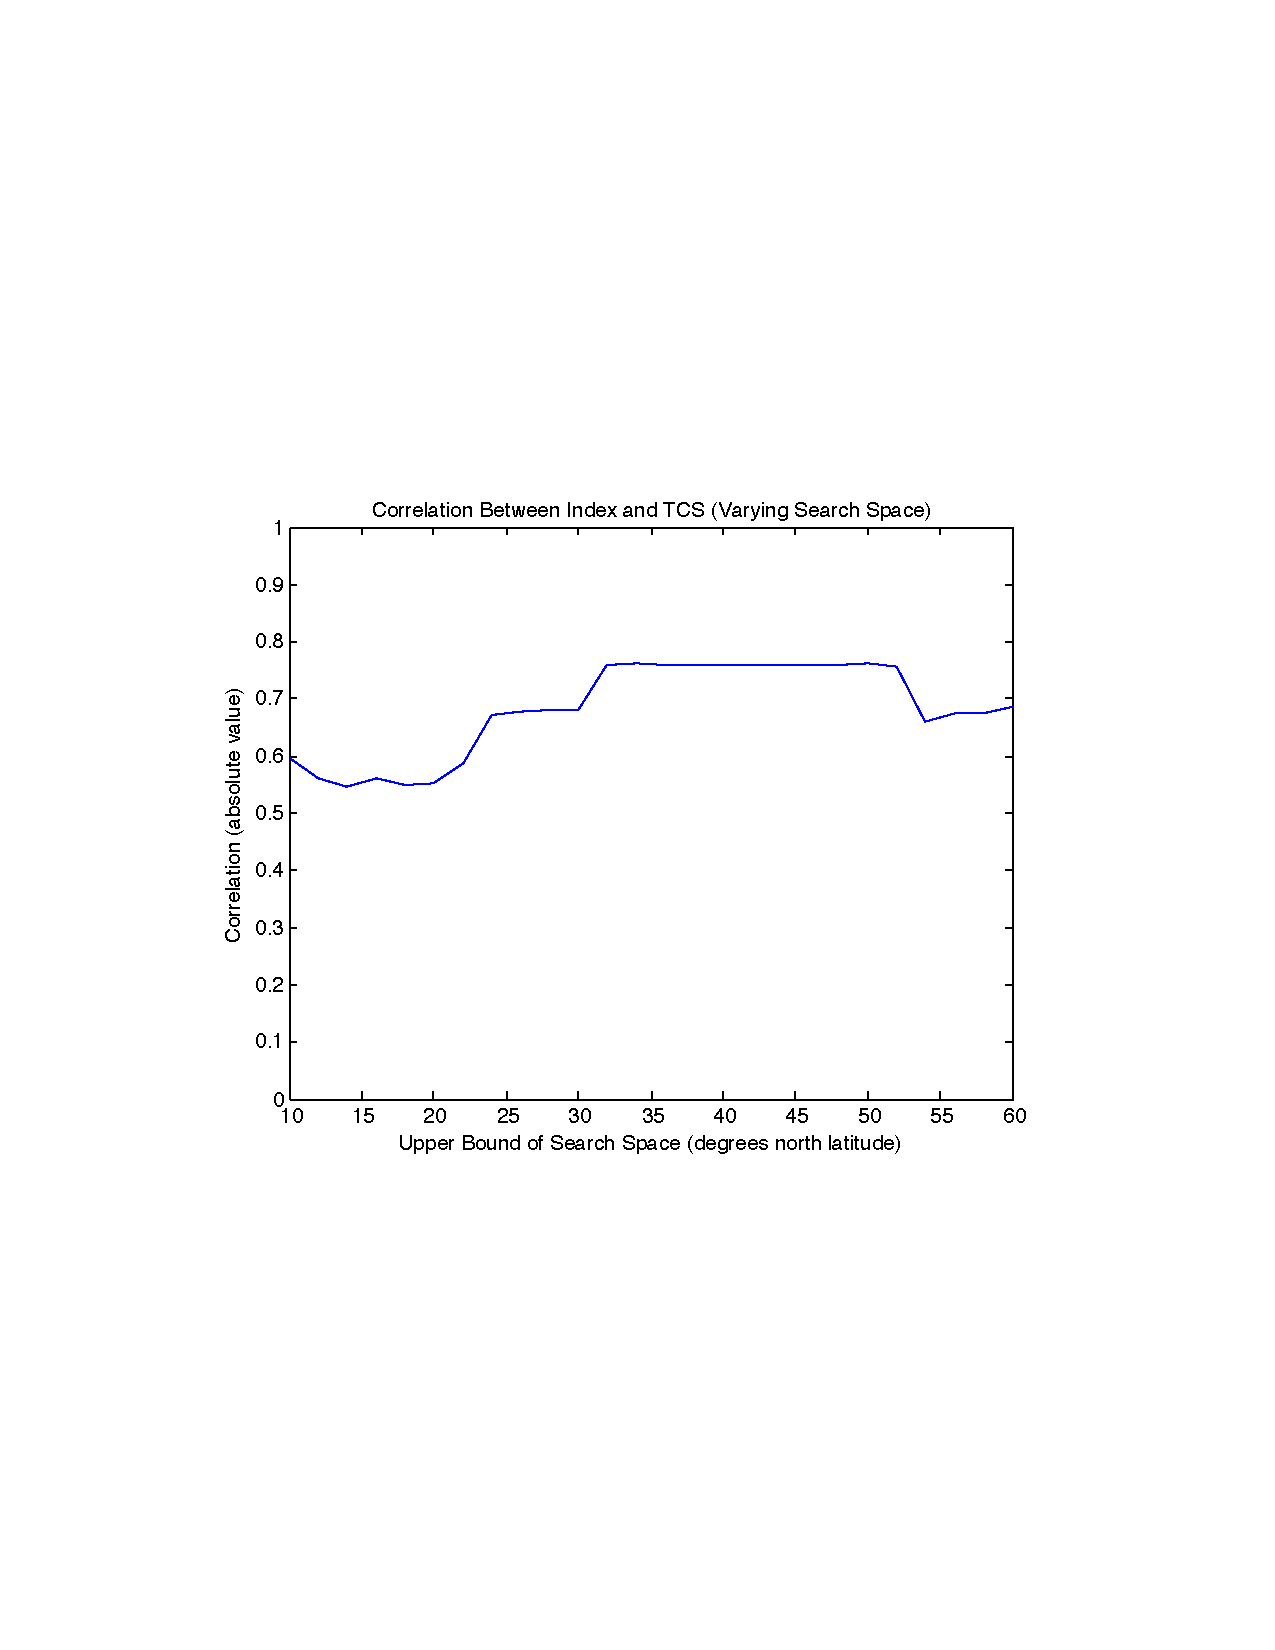
\includegraphics[width=\textwidth]{figs/sensitivityResults/northHem/TCS_Index_North.pdf}
\caption{Corr Index vs. TCs}
\label{fig:figure16}
\end{minipage}
\end{figure}
\pagebreak
\subsection{Varying Hurricane Season}

\begin{figure}[ht]
\begin{minipage}[b]{0.6\linewidth}
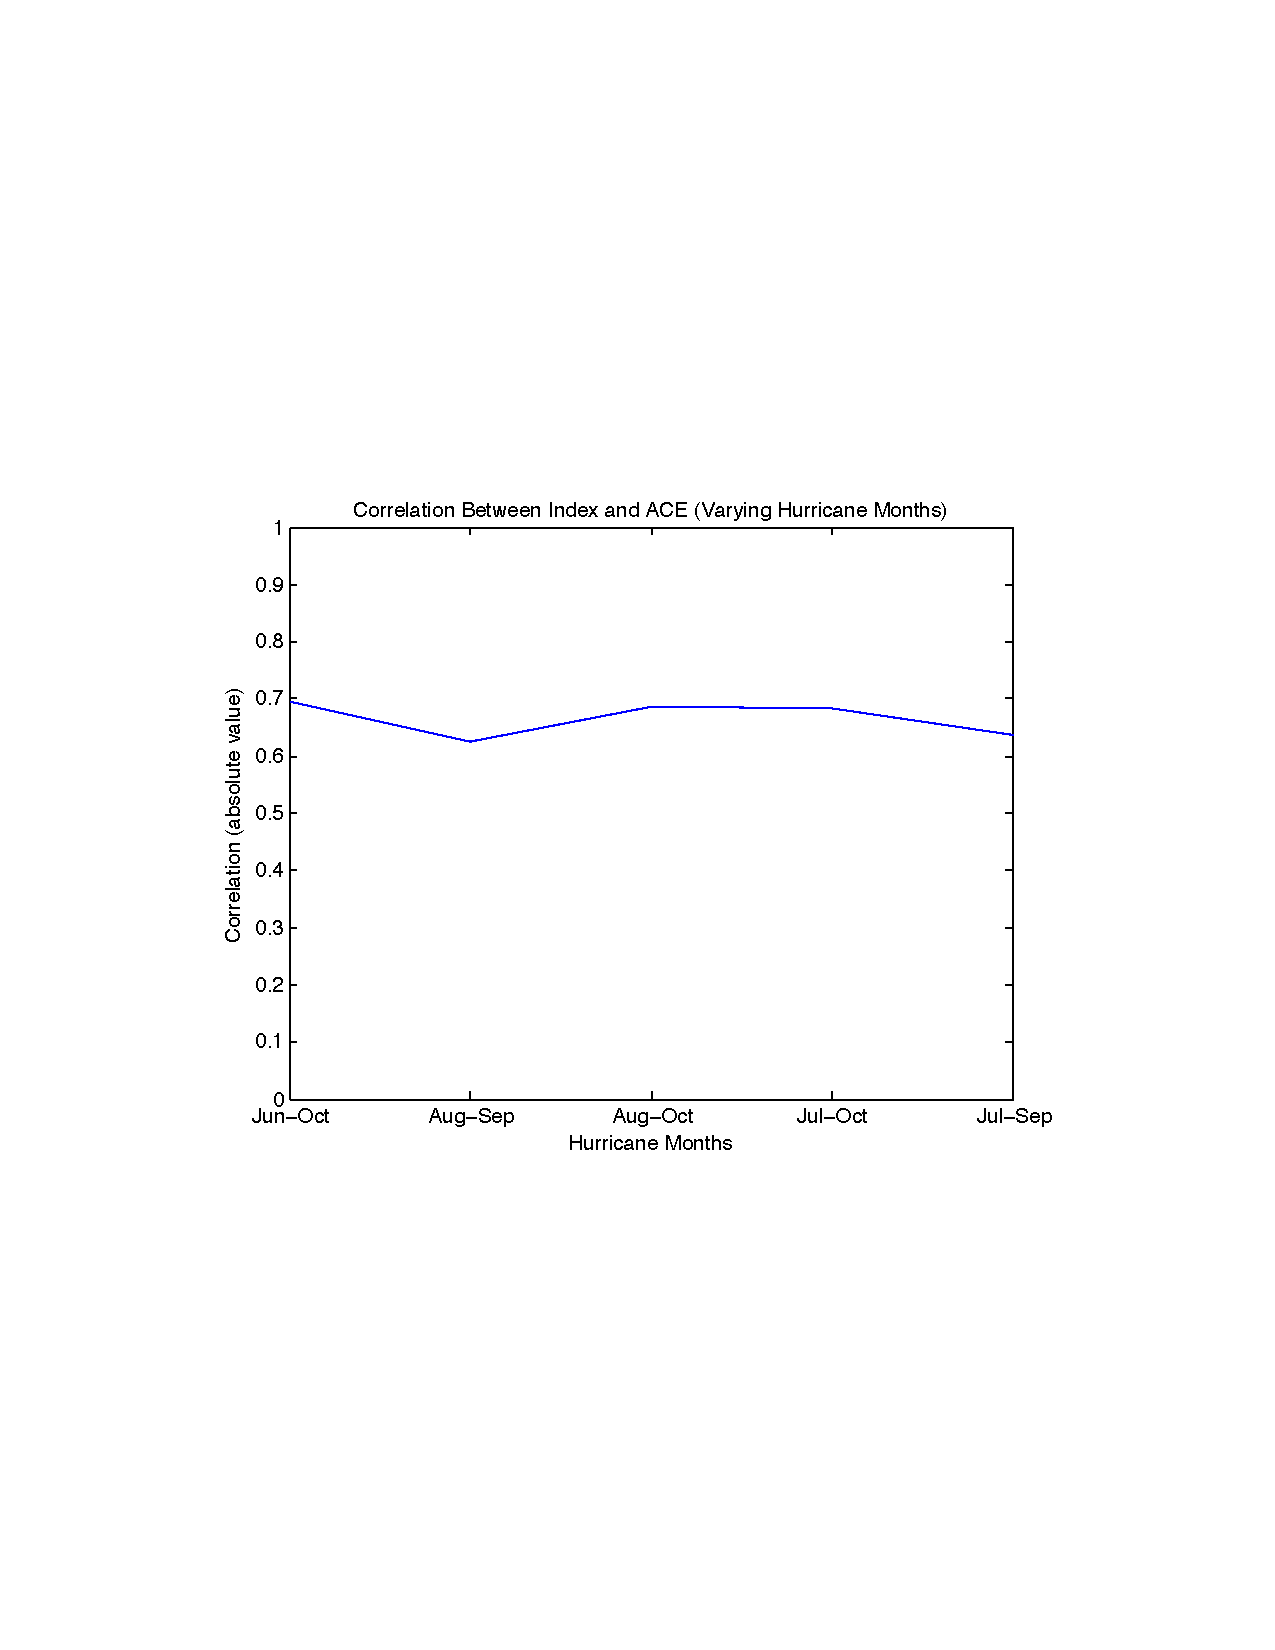
\includegraphics[width=\textwidth]{figs/sensitivityResults/hurrMonths/ACE_Index_Hurr_Months.pdf}
\caption{Corr Index vs. ACE}
\label{fig:figure17}
\end{minipage}
\hspace{0cm}
\begin{minipage}[b]{0.6\linewidth}
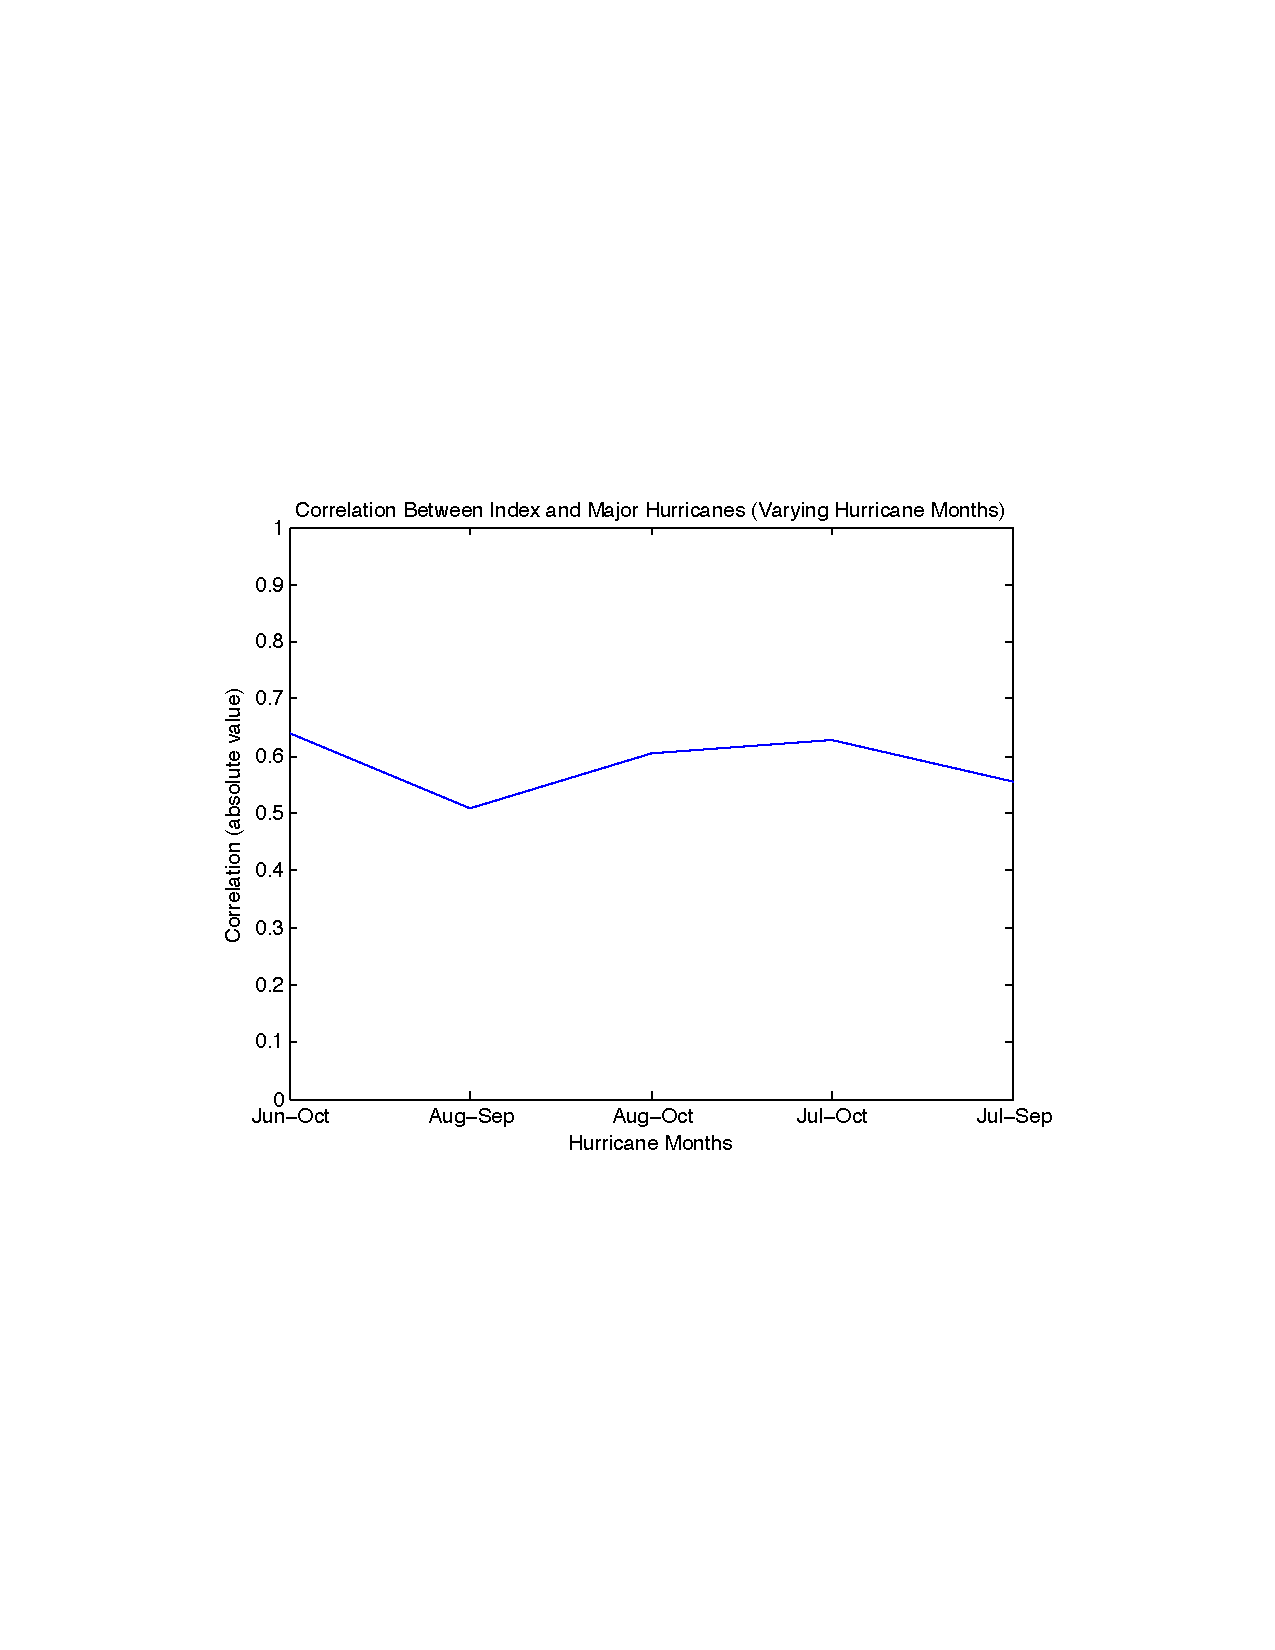
\includegraphics[width=\textwidth]{figs/sensitivityResults/hurrMonths/Major_Hurricanes_Index_Hurr_Months.pdf}
\caption{Corr Index vs. Major Hurricanes}
\label{fig:figure18}
\end{minipage}
\end{figure}
\begin{figure}[ht]
\begin{minipage}[b]{0.6\linewidth}
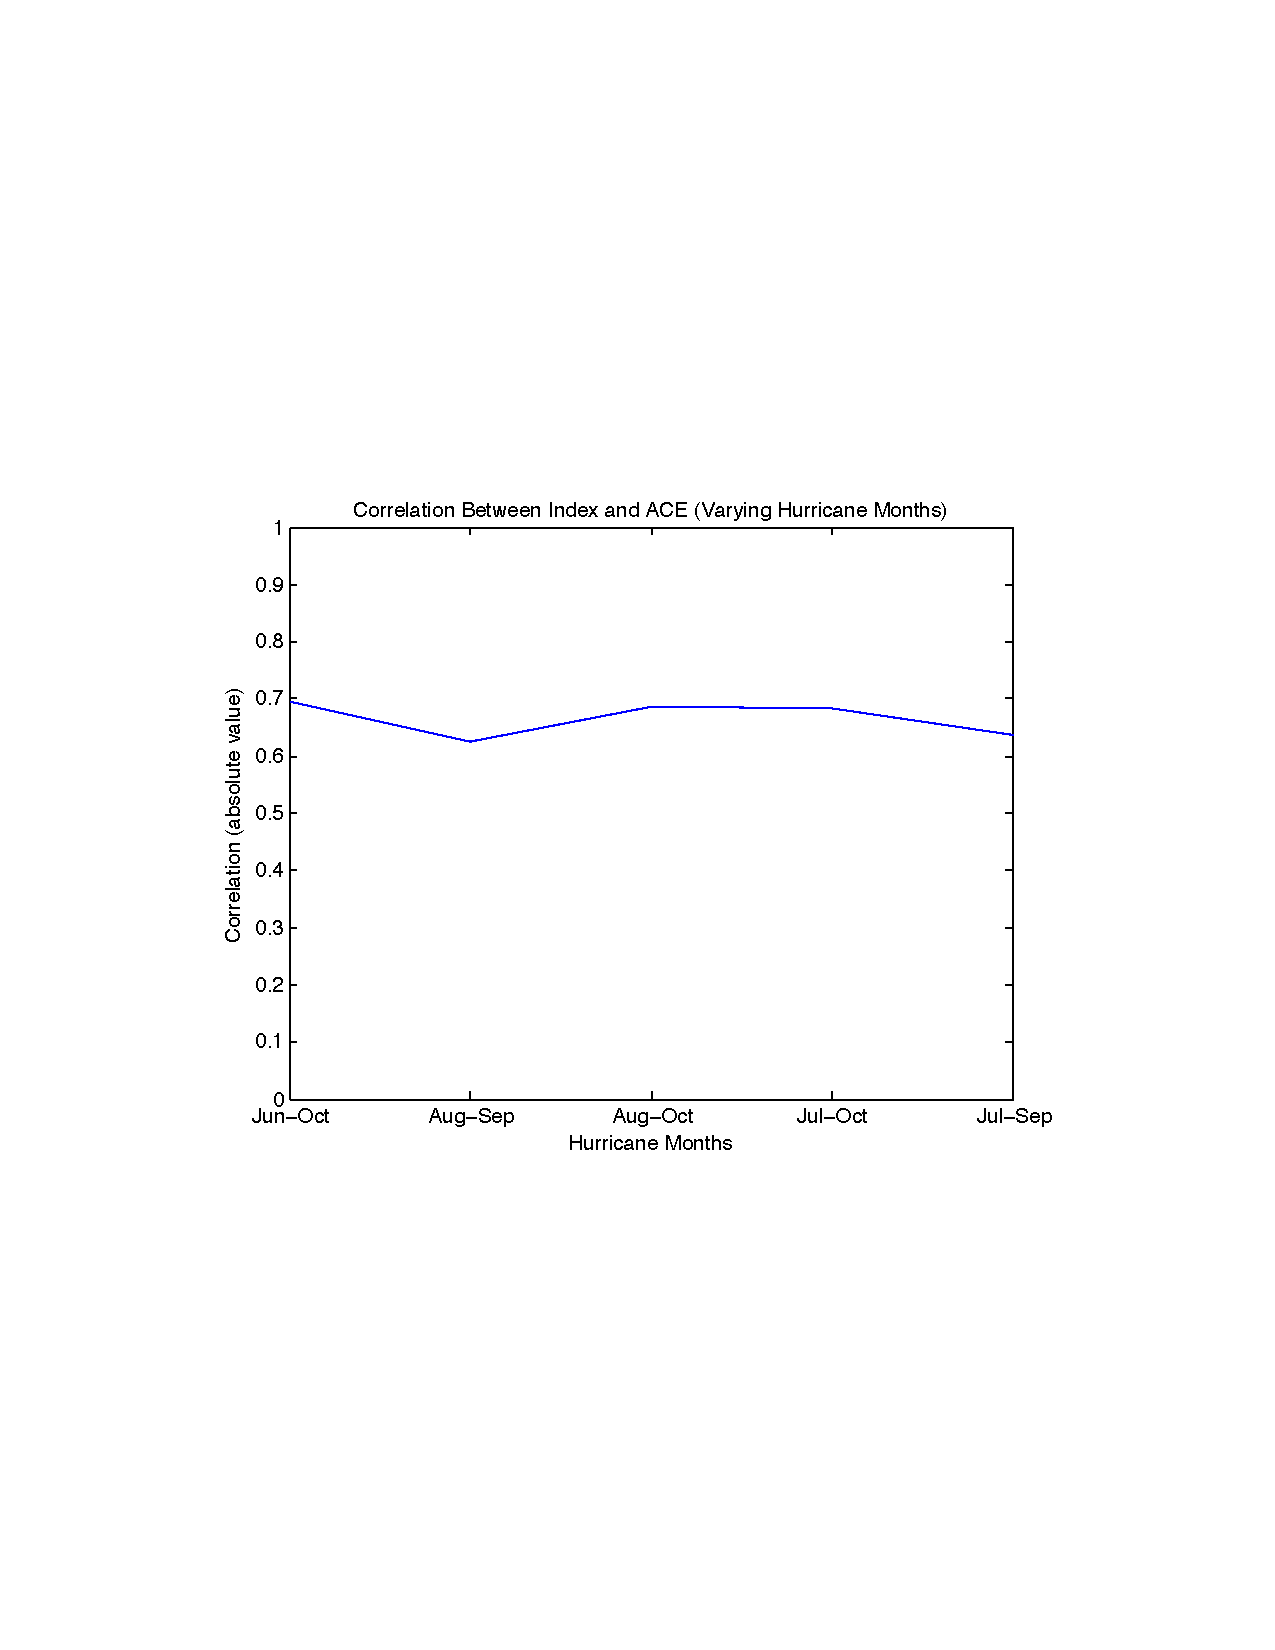
\includegraphics[width=\textwidth]{figs/sensitivityResults/hurrMonths/ACE_Index_Hurr_Months.pdf}
\caption{Corr Index vs. ACE}
\label{fig:figure19}
\end{minipage}
\hspace{0cm}
\begin{minipage}[b]{0.6\linewidth}
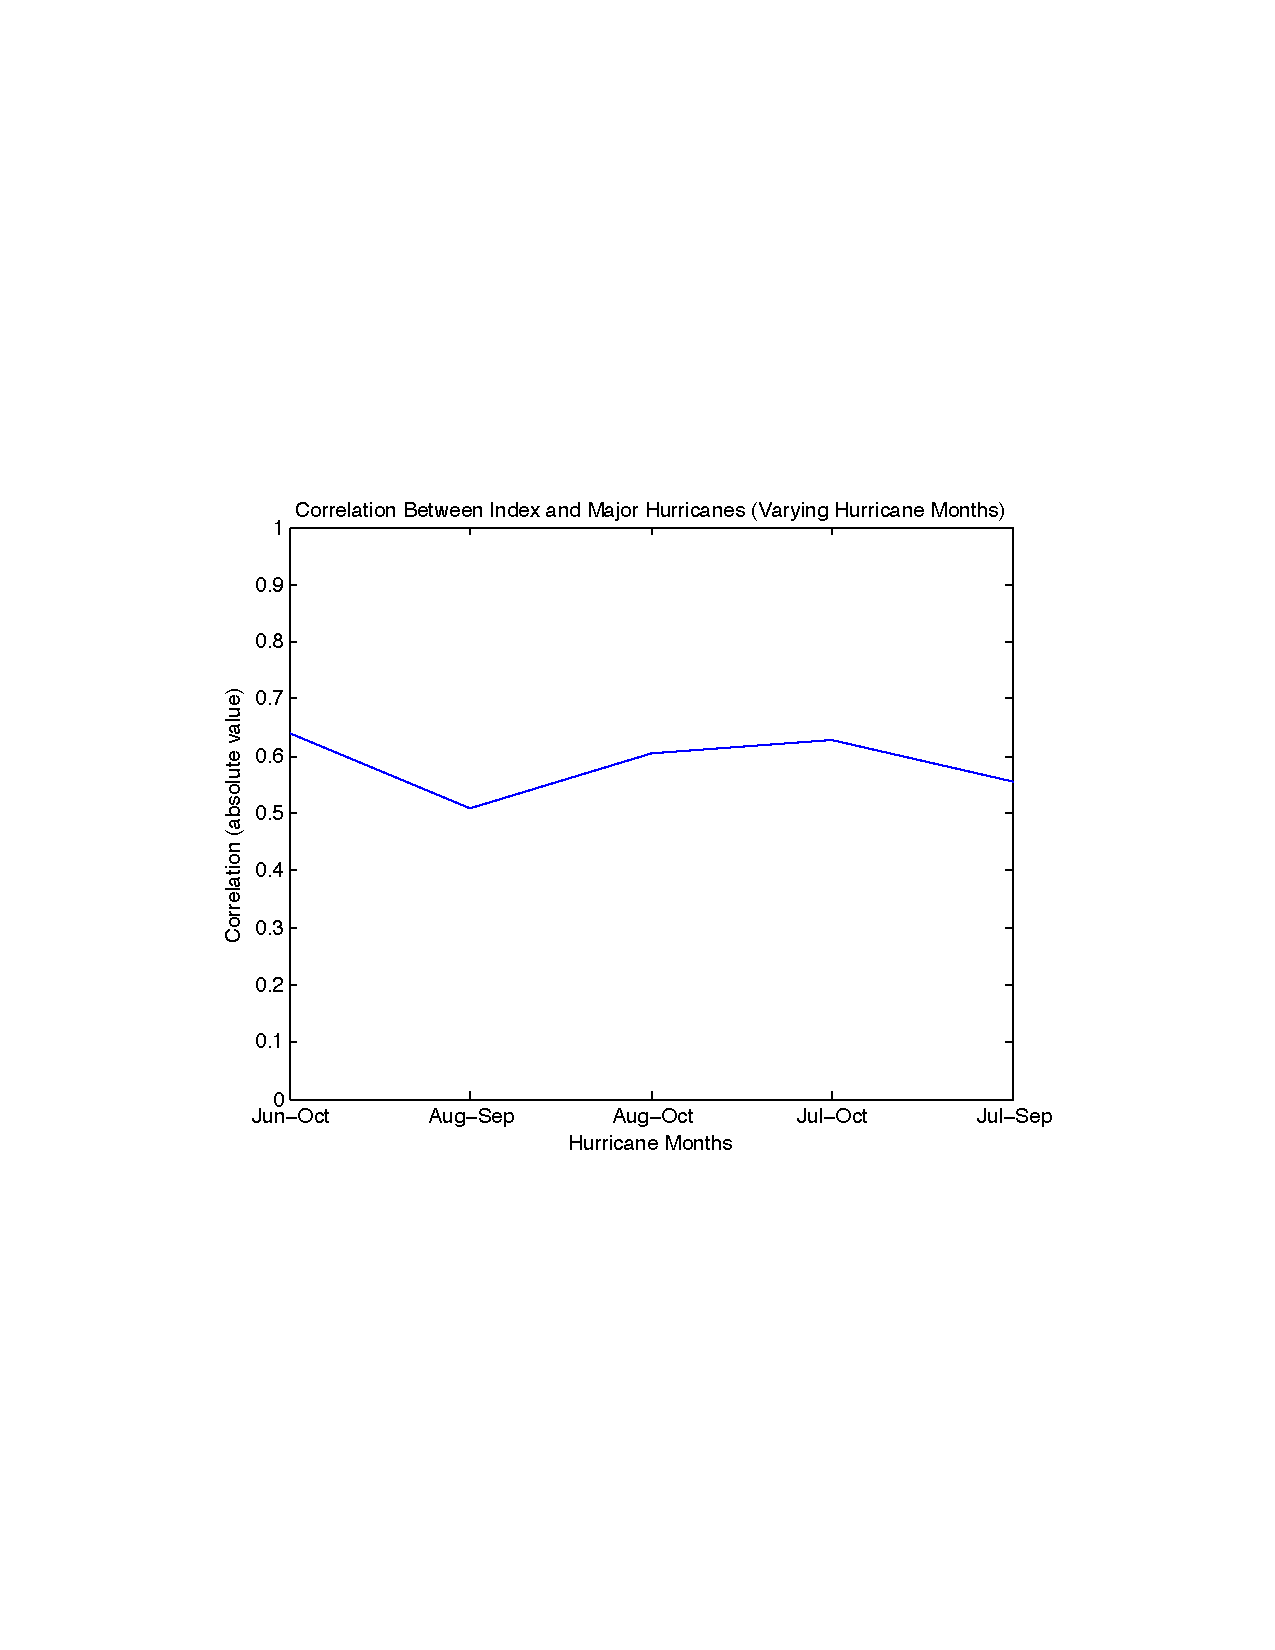
\includegraphics[width=\textwidth]{figs/sensitivityResults/hurrMonths/Major_Hurricanes_Index_Hurr_Months.pdf}
\caption{Corr Index vs. Major Hurricanes}
\label{fig:figure20}
\end{minipage}
\end{figure}

\pagebreak
\section{Difference Composite Maps}
\begin{figure}[ht]
\begin{minipage}[b]{0.6\linewidth}
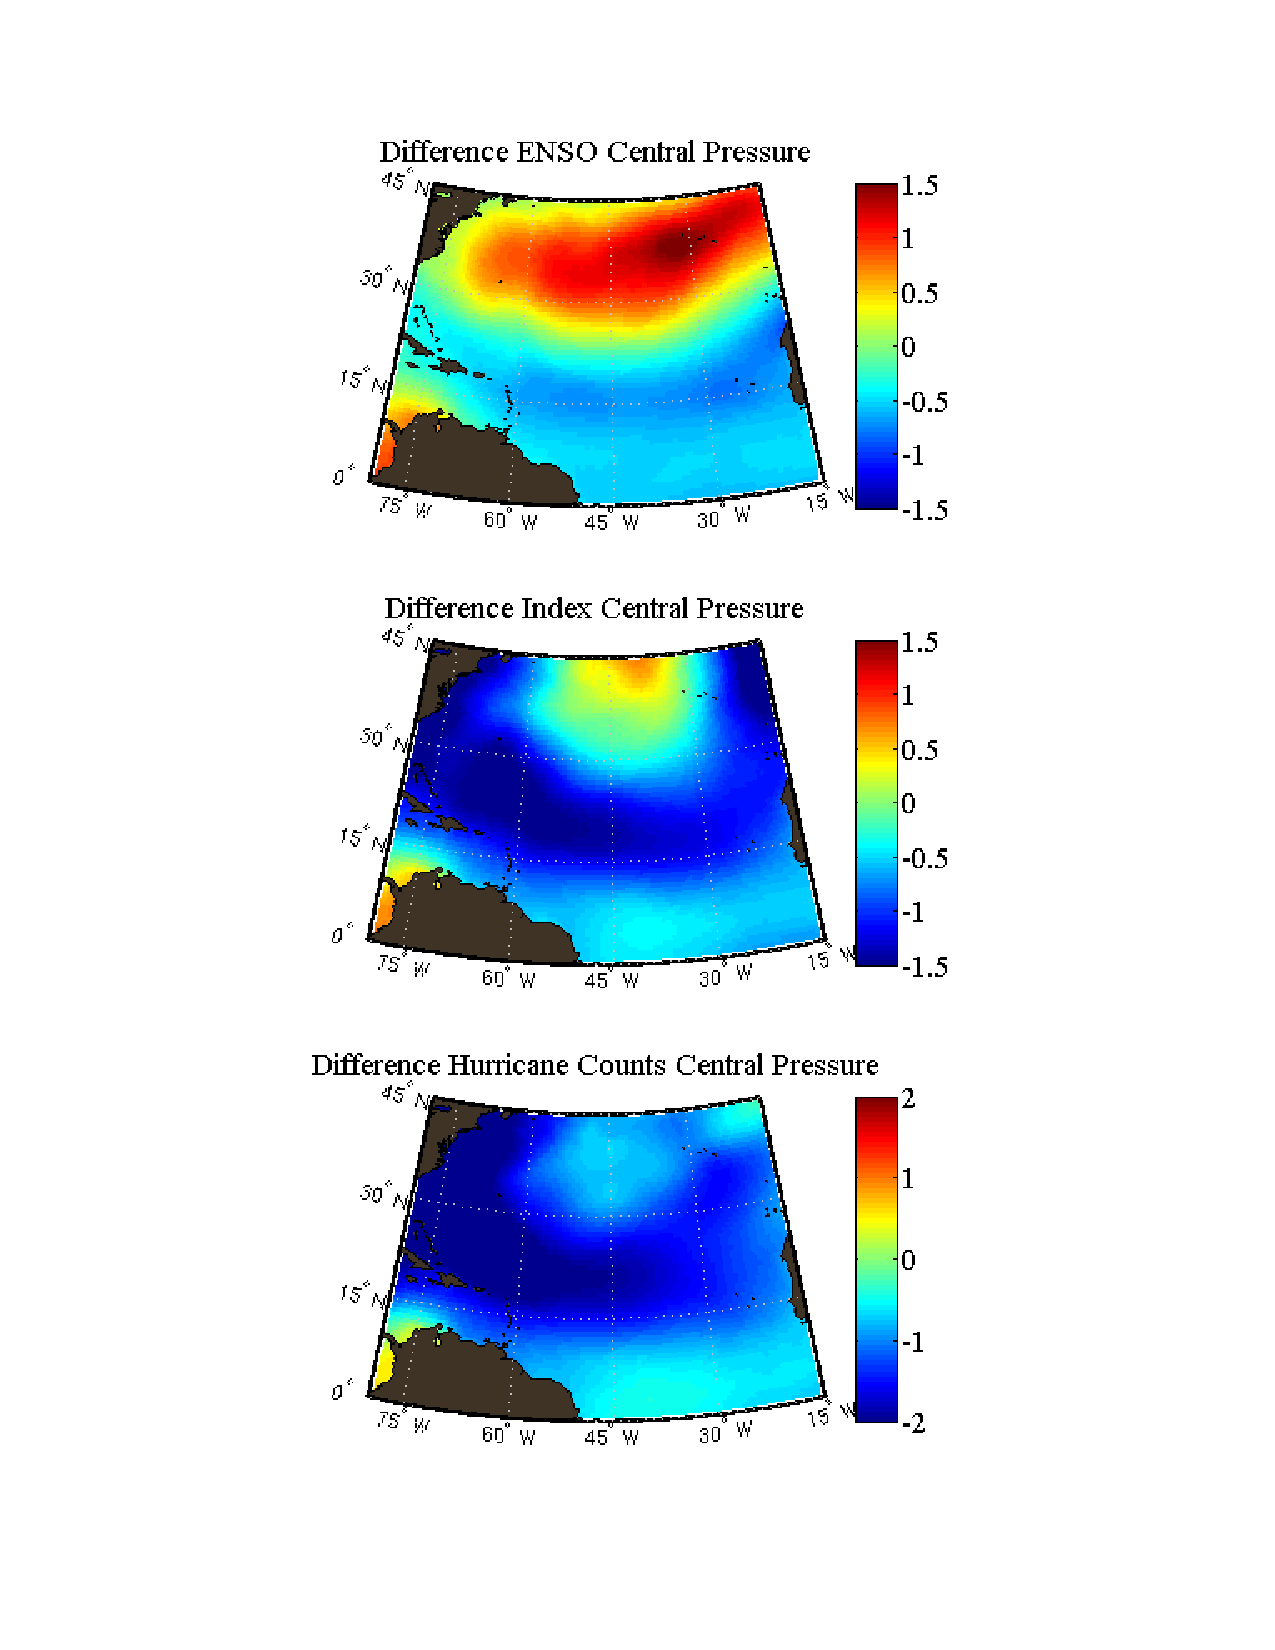
\includegraphics[width=\textwidth]{figs/sensitivityResults/compositeMaps/centralPressureAtlanticMap.pdf}
\caption{Diff Pressure Composites}
\label{fig:figure21}
\end{minipage}
\hspace{0cm}
\begin{minipage}[b]{0.6\linewidth}
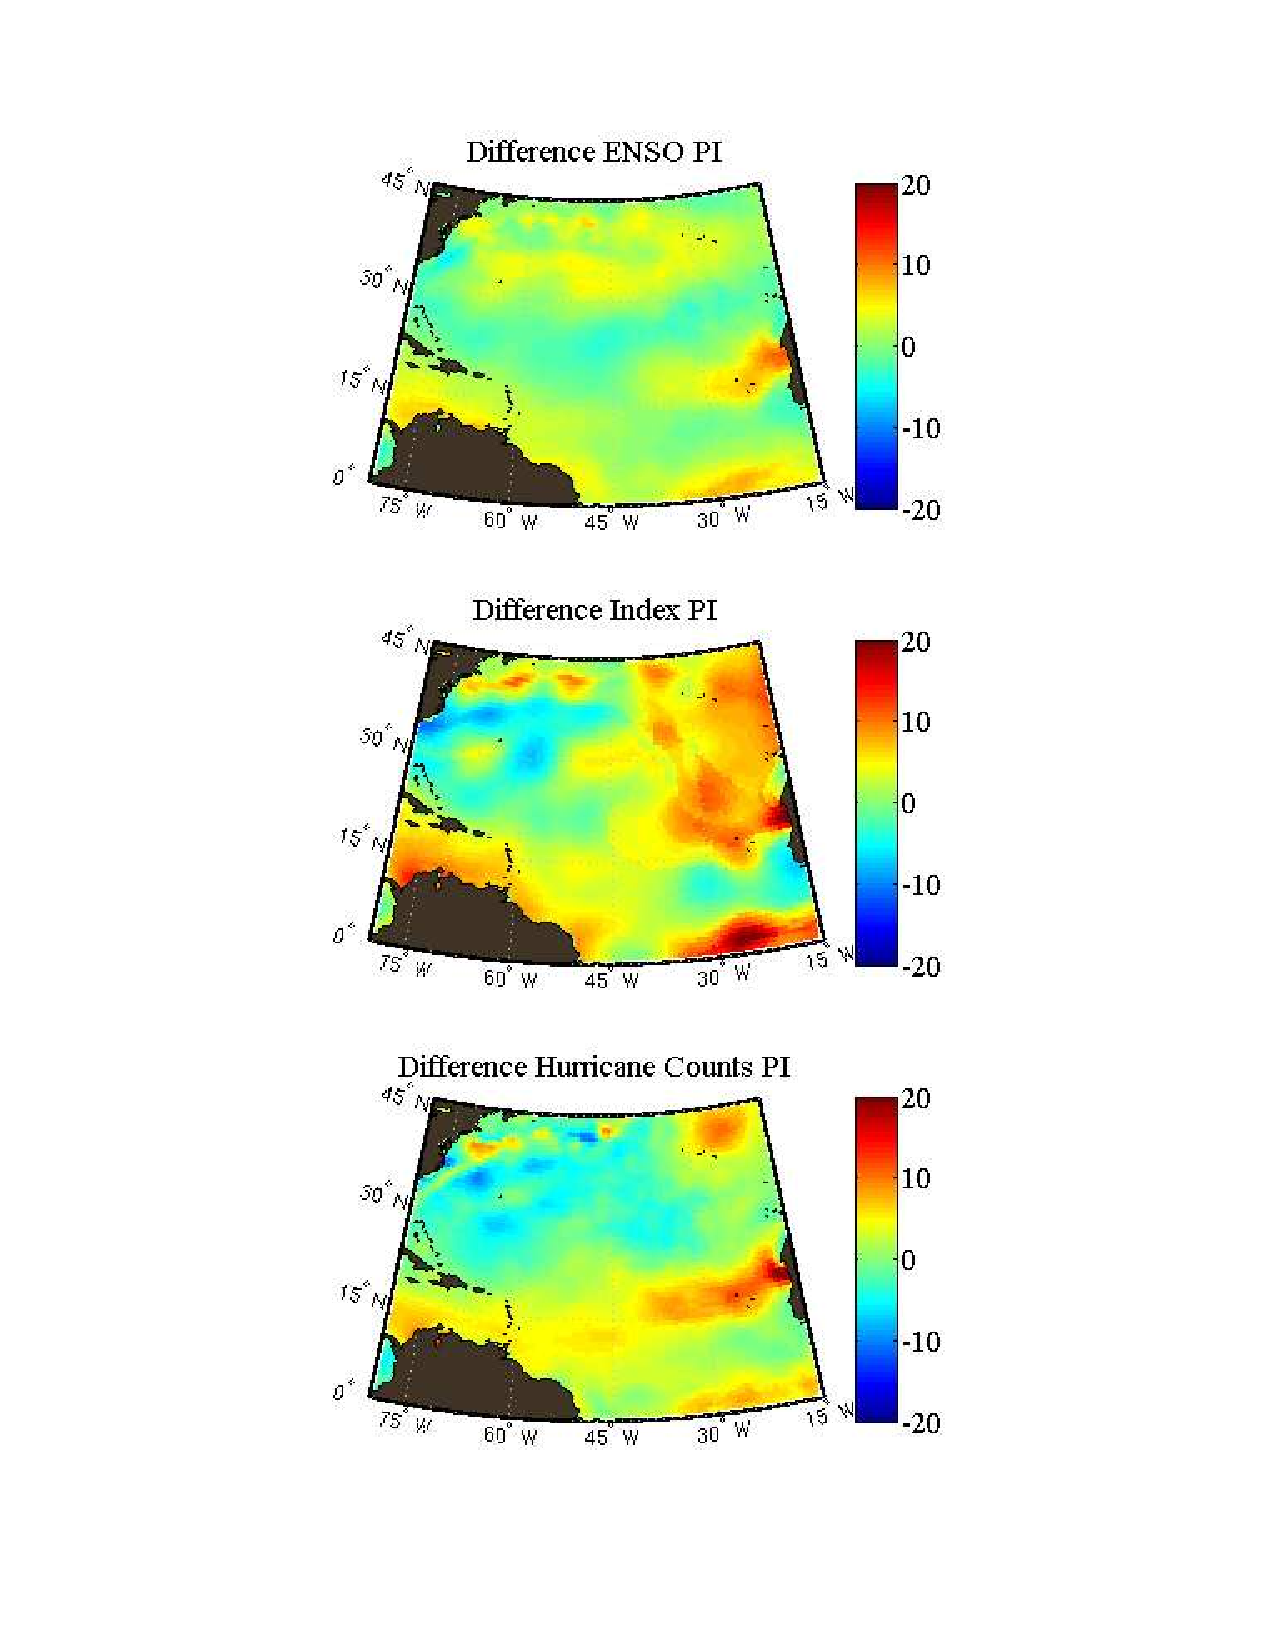
\includegraphics[width=\textwidth]{figs/sensitivityResults/compositeMaps/diffPIAtlanticComposites.pdf}
\caption{Diff PI Composites}
\label{fig:figure22}
\end{minipage}
\end{figure}

\pagebreak
\begin{figure}[ht]
\begin{minipage}[b]{0.6\linewidth}
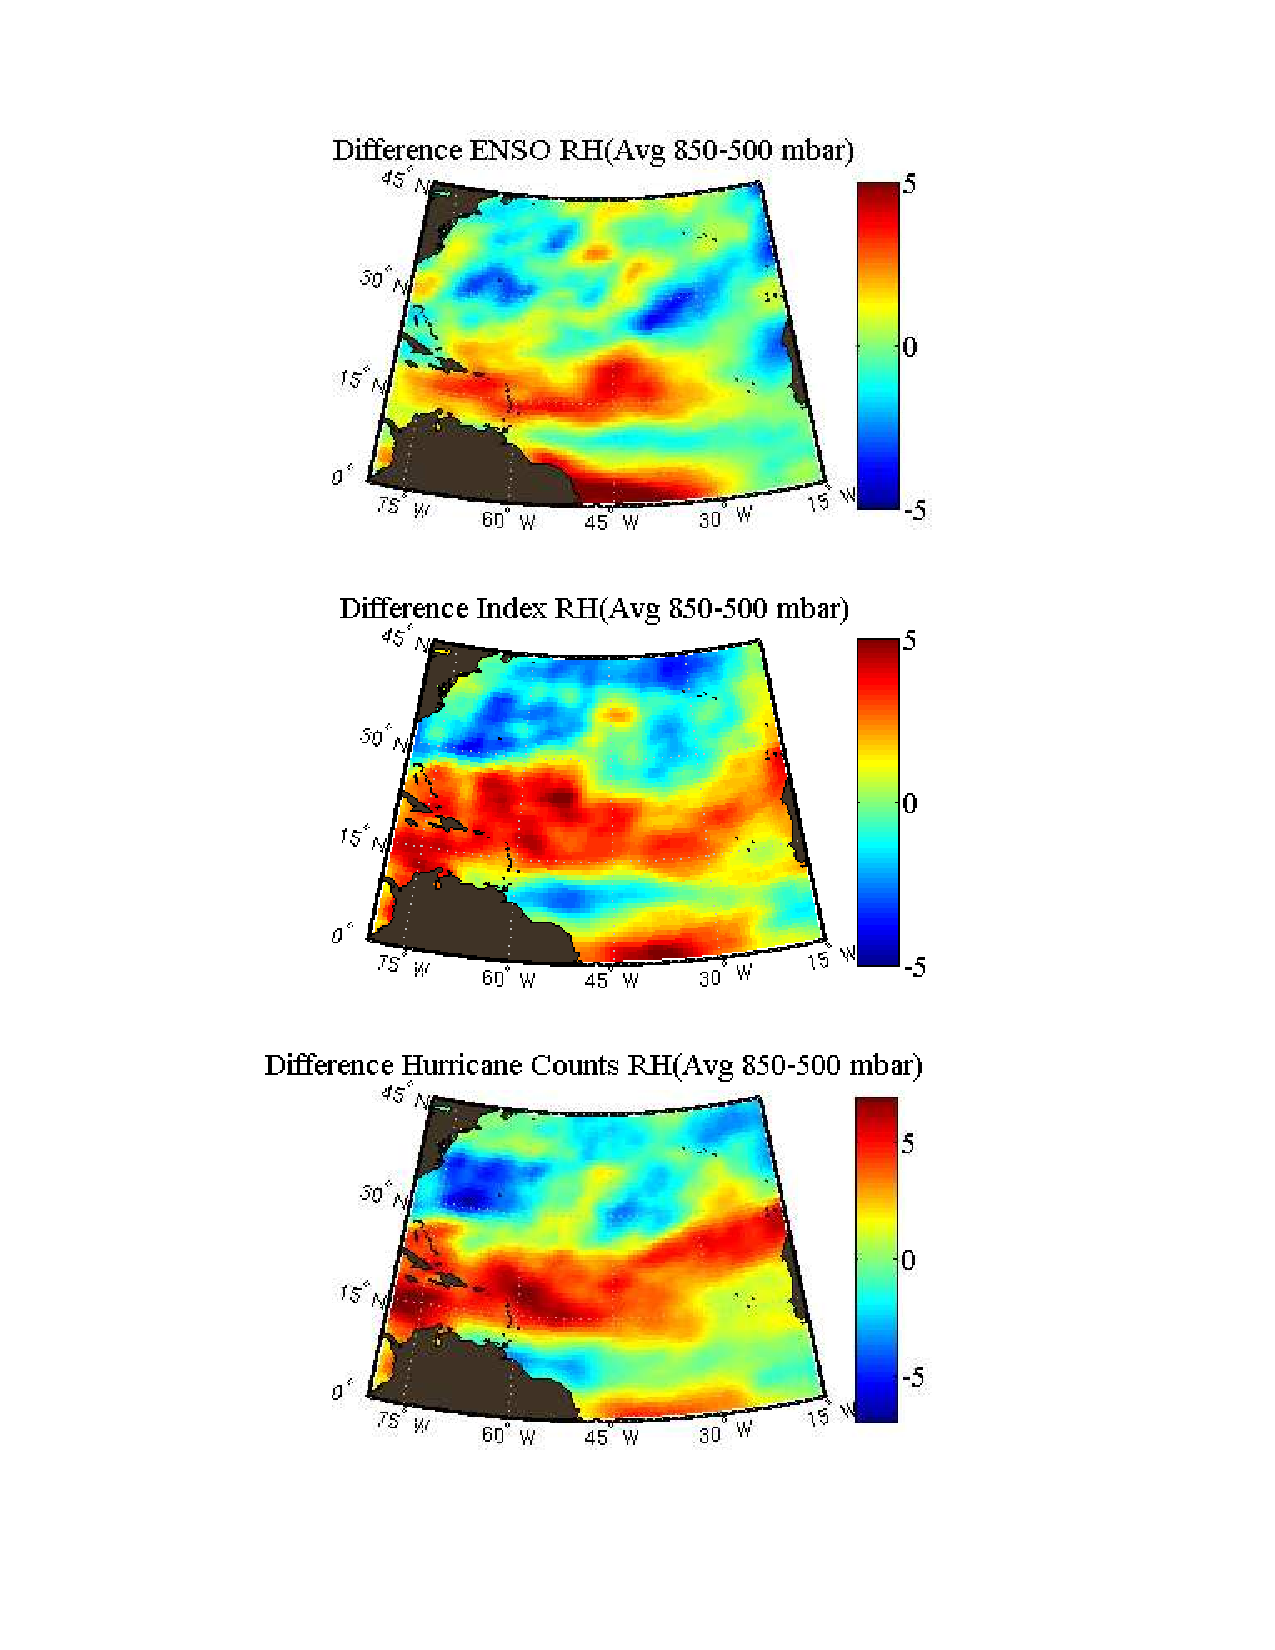
\includegraphics[width=\textwidth]{figs/sensitivityResults/compositeMaps/diffRHCompositesAtlanticMap.pdf}
\caption{Diff Relative Humidity}
\label{fig:figure23}
\end{minipage}
\hspace{0cm}
\begin{minipage}[b]{0.6\linewidth}
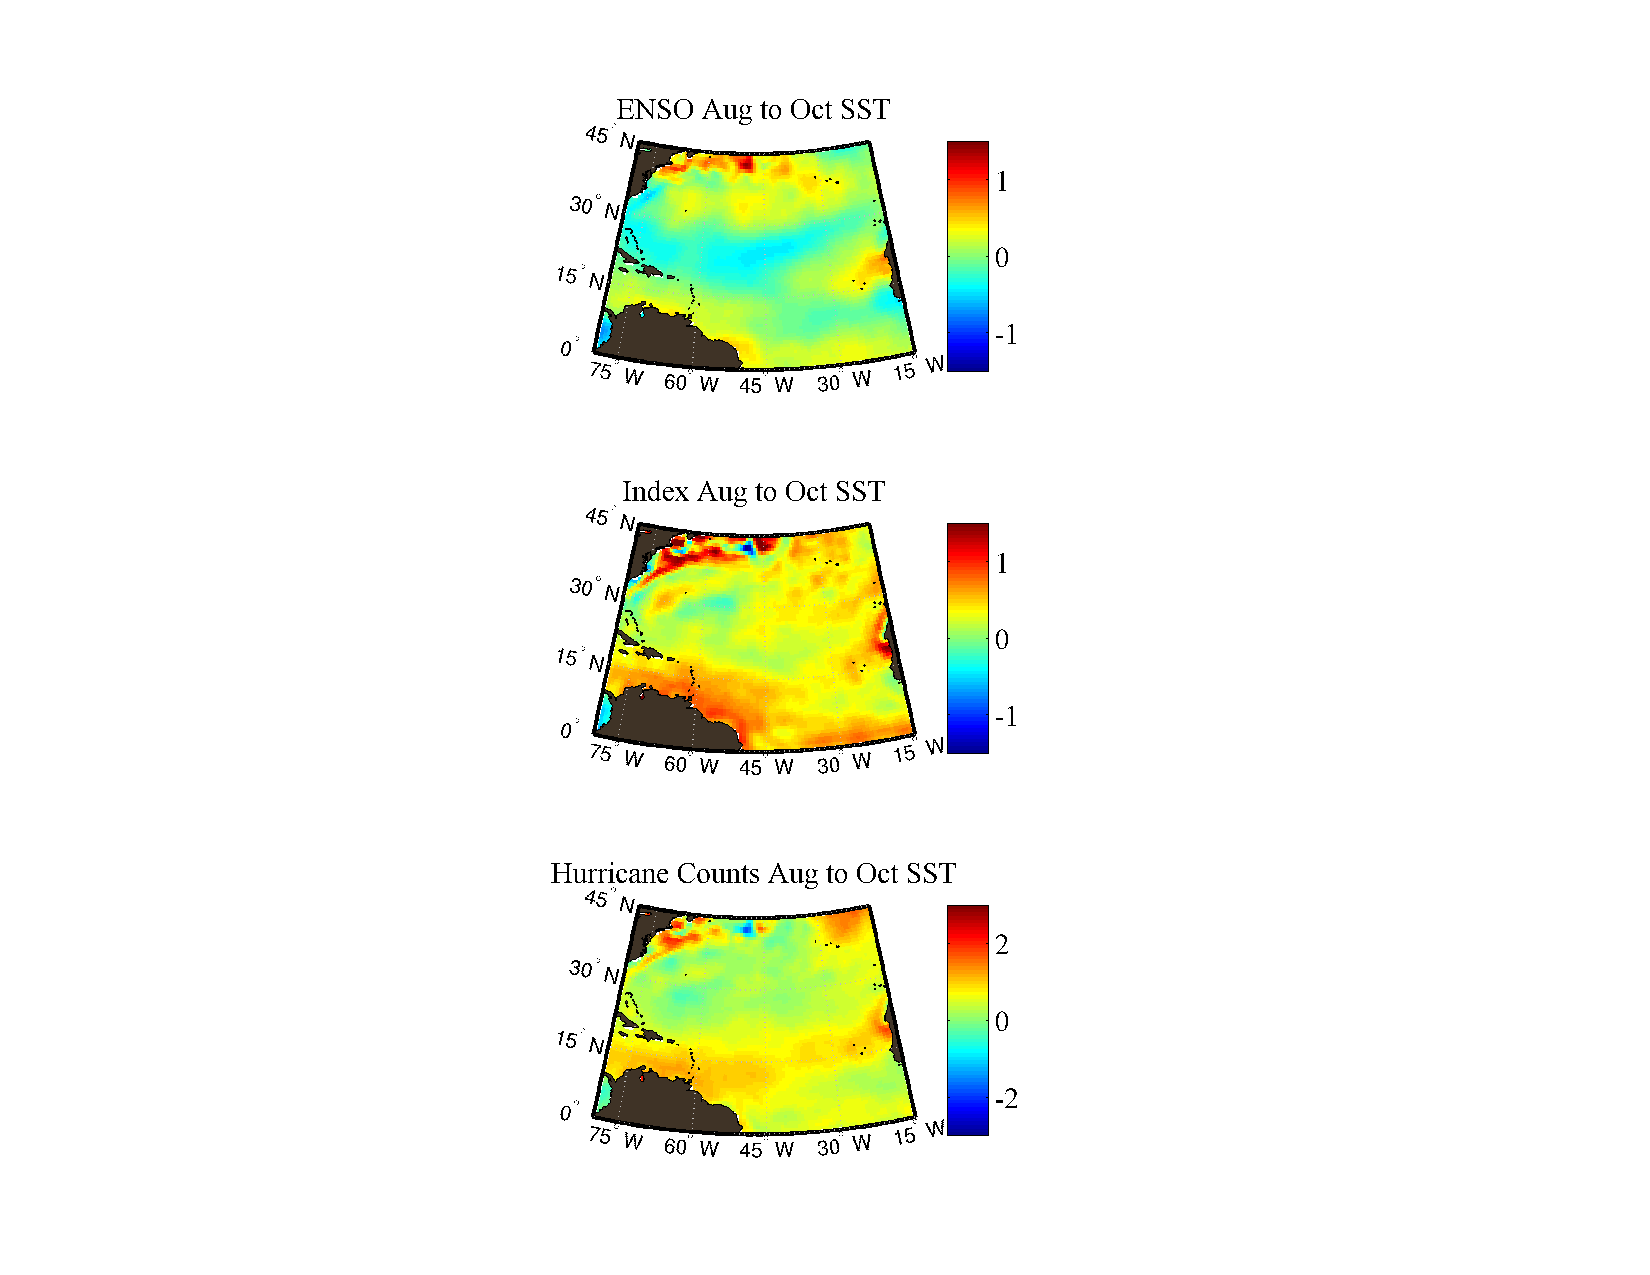
\includegraphics[width=\textwidth]{figs/sensitivityResults/compositeMaps/diffSSTCompositesAugToOct.pdf}
\caption{Diff SST Composites}
\label{fig:figure24}
\end{minipage}
\end{figure}

\pagebreak
\begin{figure}[ht]
\begin{minipage}[b]{0.6\linewidth}
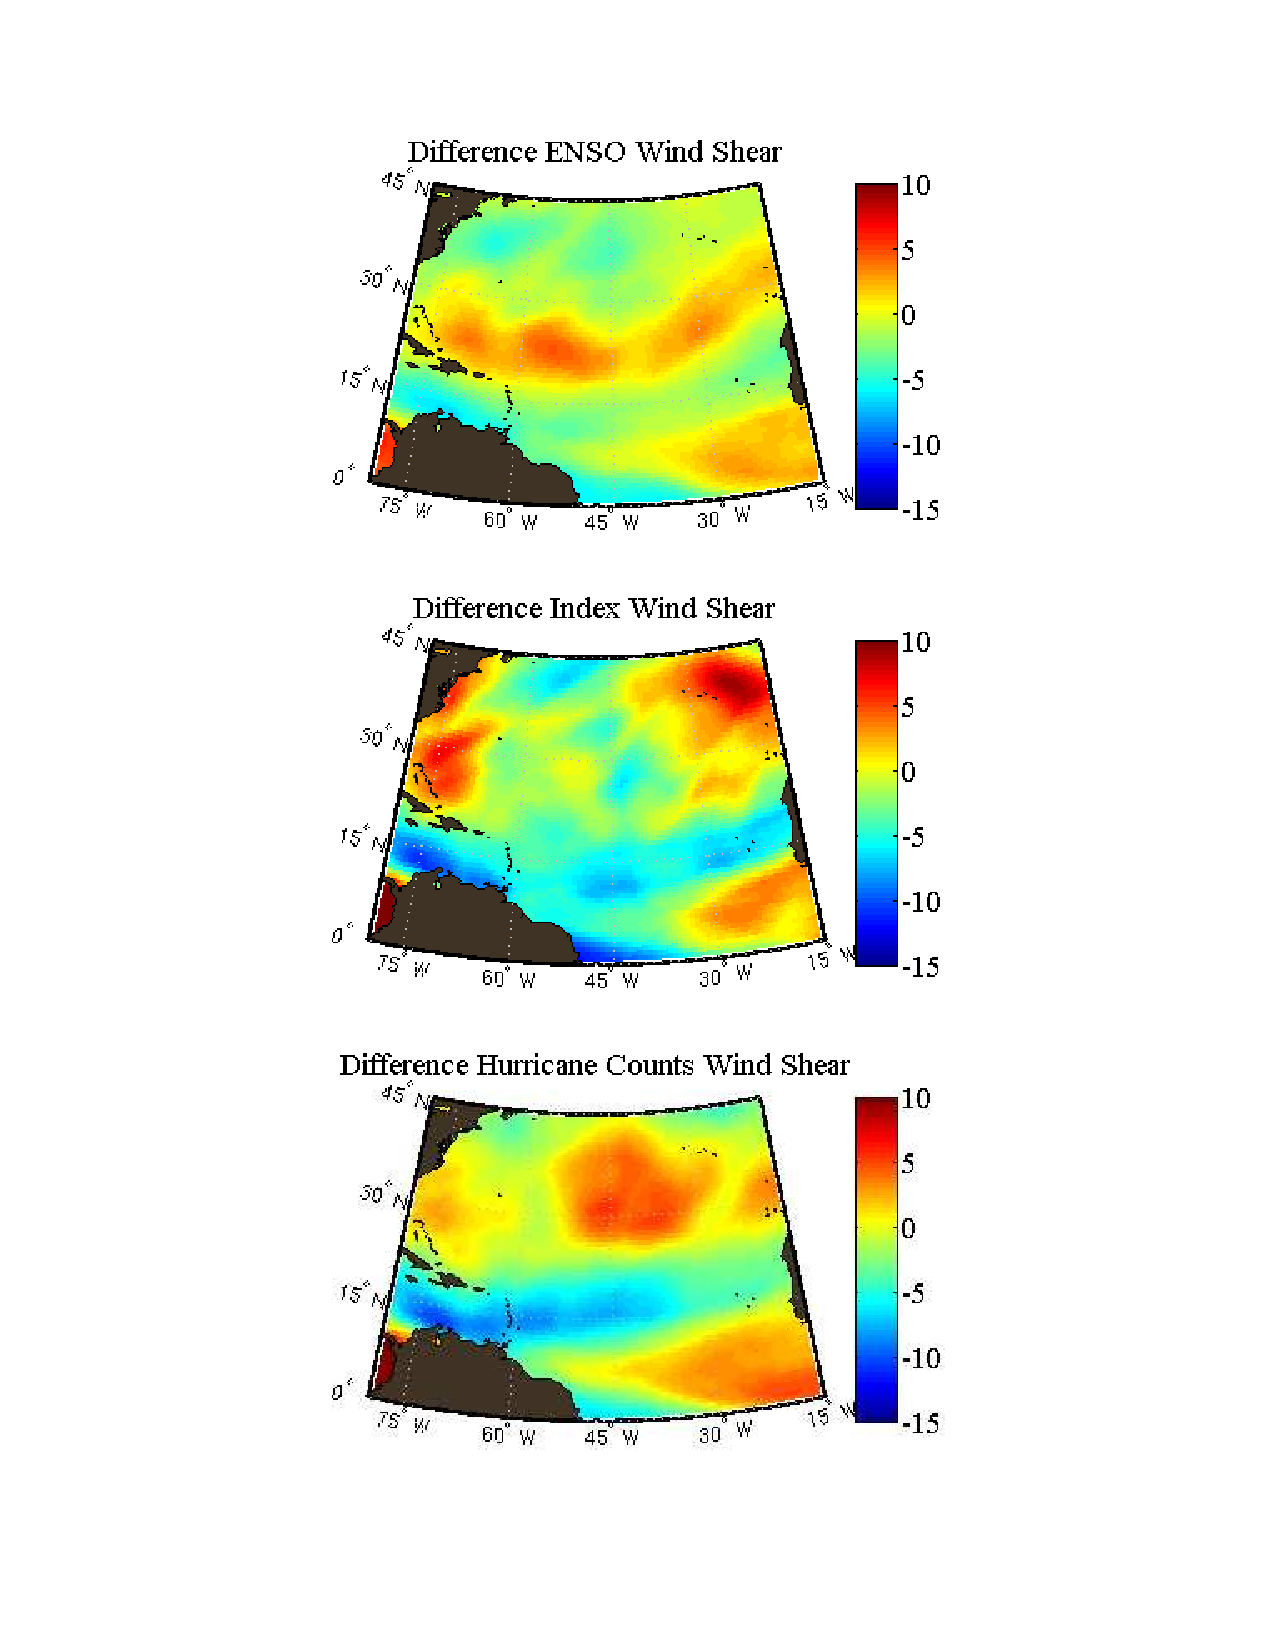
\includegraphics[width=\textwidth]{figs/sensitivityResults/compositeMaps/diffWindShearAtlanticComposites.pdf}
\caption{Diff Wind Shear}
\label{fig:figure25}
\end{minipage}
\hspace{0cm}
\begin{minipage}[b]{0.6\linewidth}
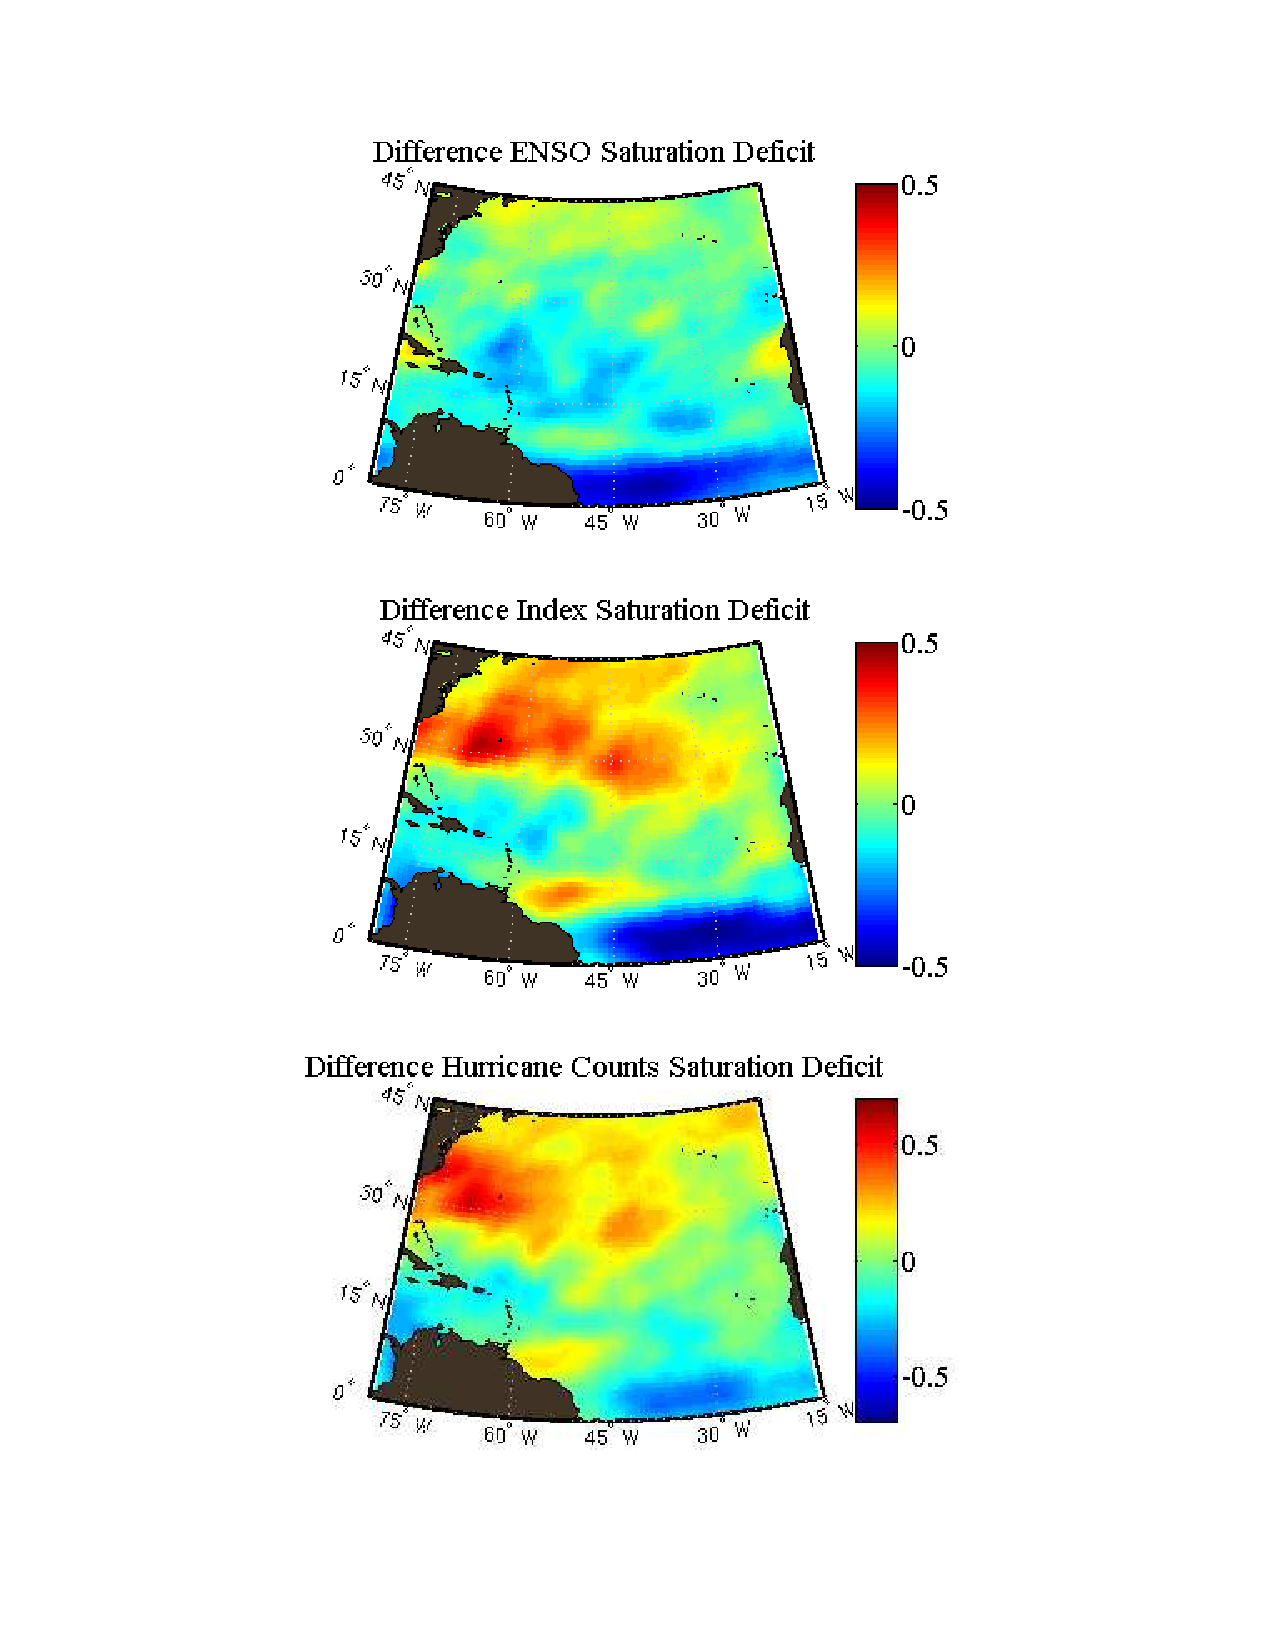
\includegraphics[width=\textwidth]{figs/sensitivityResults/compositeMaps/satDefAtlanticMap.pdf}
\caption{Diff Saturation Deficit}
\label{fig:figure26}
\end{minipage}
\end{figure}

\pagebreak
\section{Average Difference Bar Graphs}
\begin{figure}[ht]
\begin{minipage}[b]{0.6\linewidth}
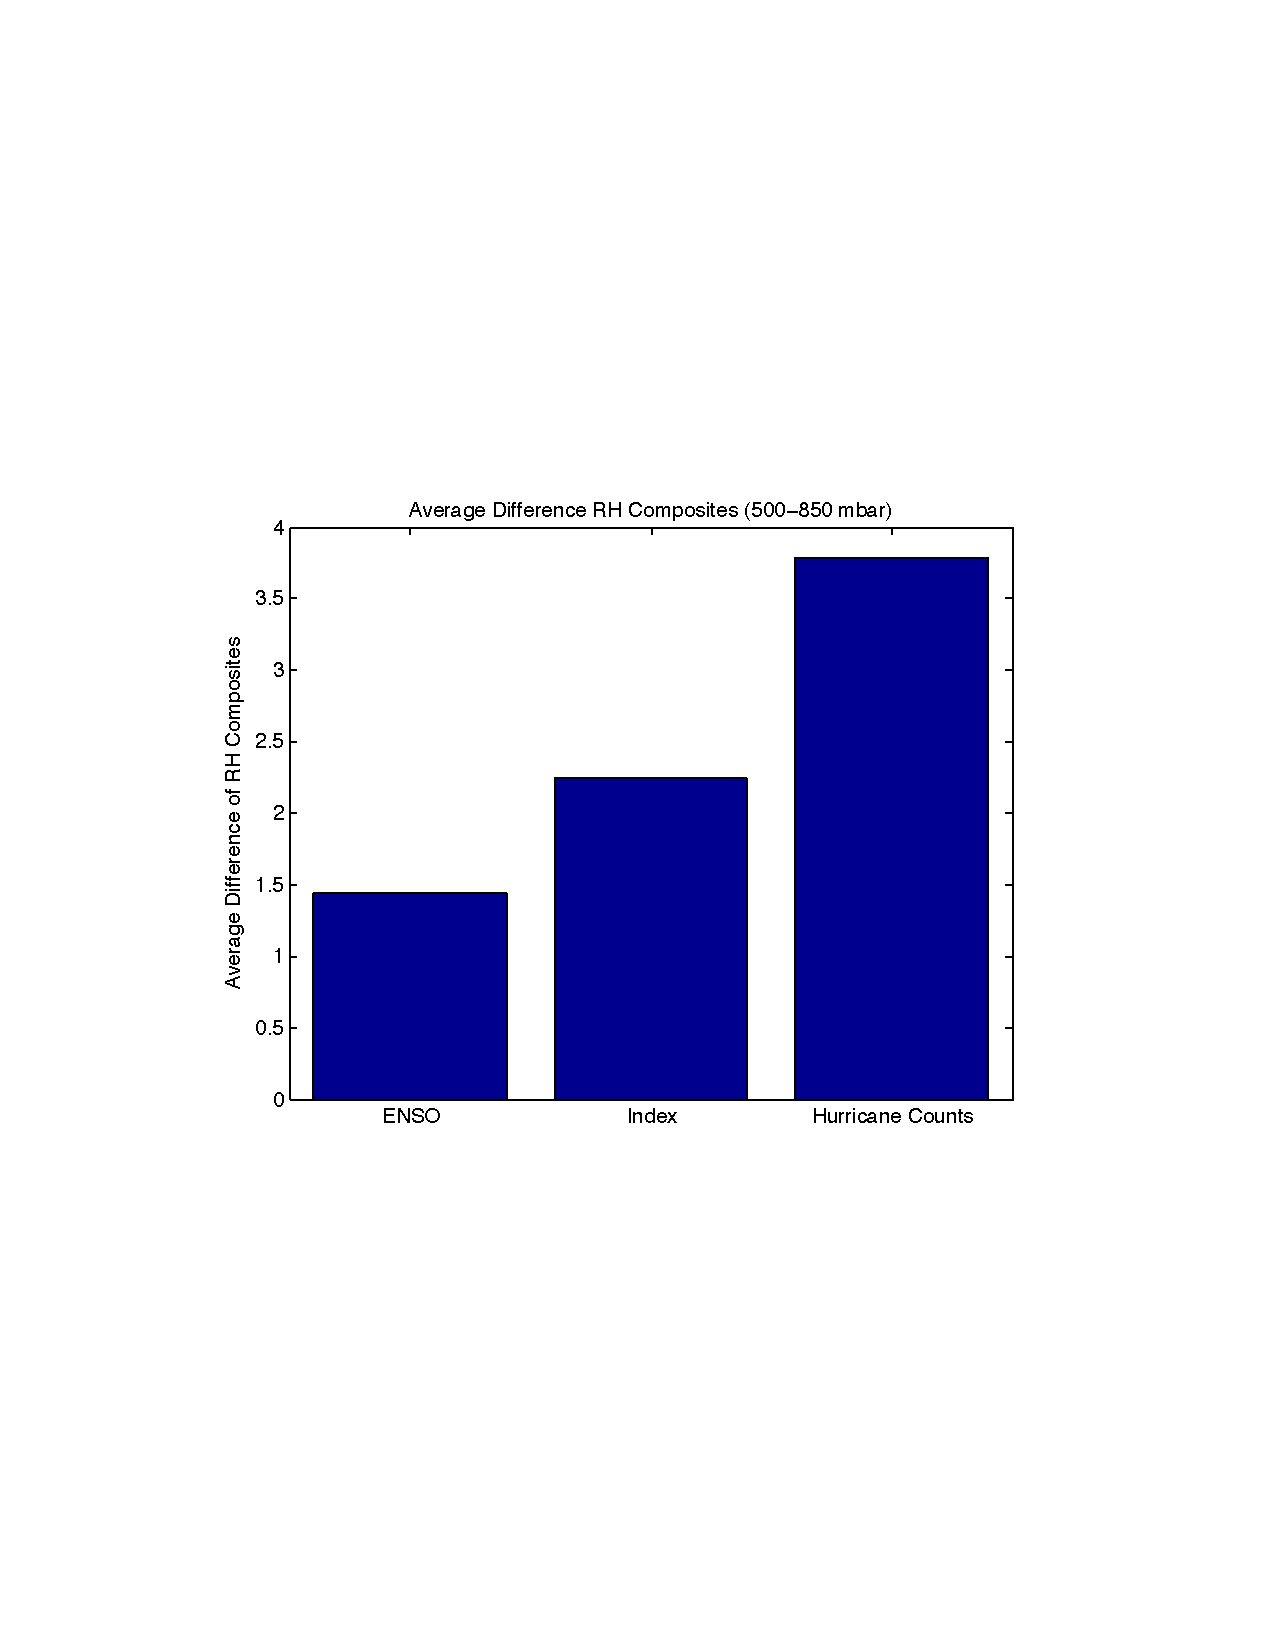
\includegraphics[width=\textwidth]{figs/sensitivityResults/compositeBarGraphs/RHBarGraph.pdf}
\caption{Avg Diff Relative Humidity}
\label{fig:figure27}
\end{minipage}
\hspace{0cm}
\begin{minipage}[b]{0.6\linewidth}
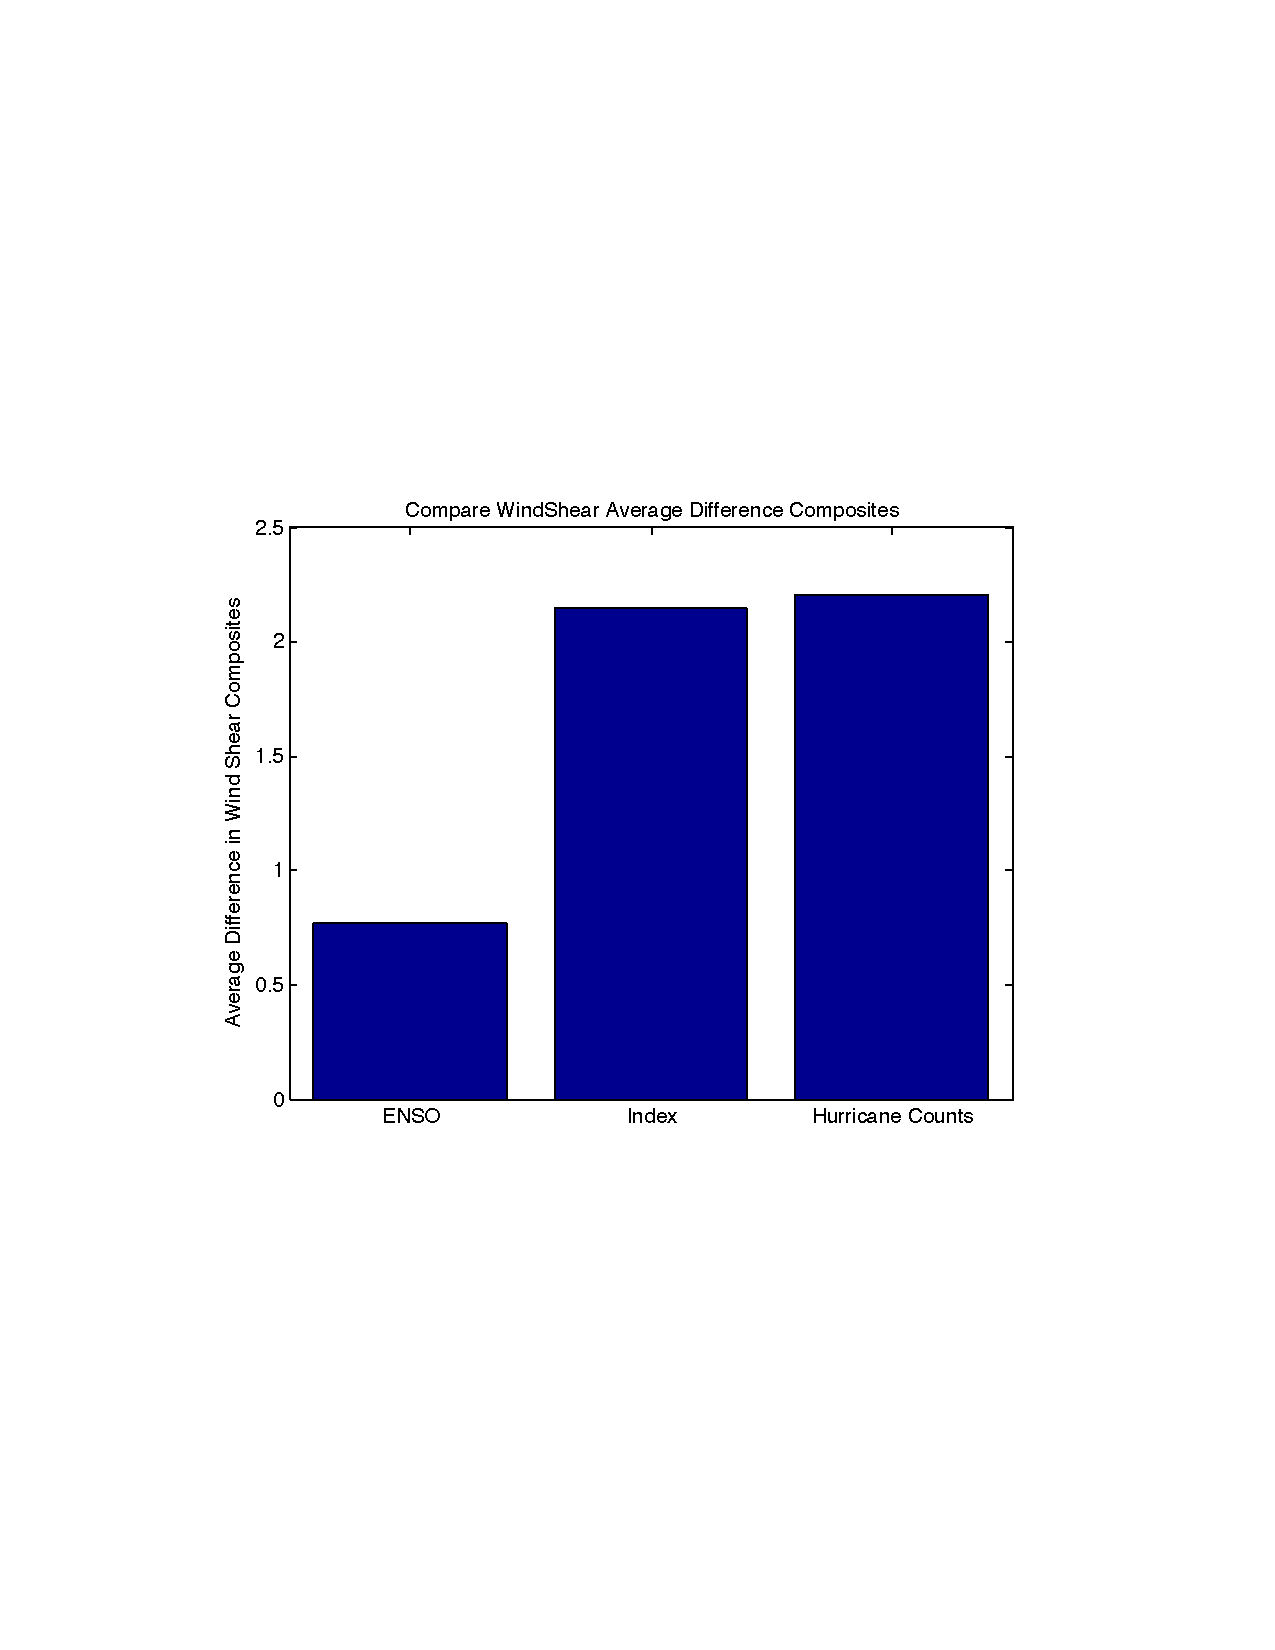
\includegraphics[width=\textwidth]{figs/sensitivityResults/compositeBarGraphs/avgDiffWindShearBarGraph.pdf}
\caption{Avg Diff Wind Shear (between 850-200mbar)}
\label{fig:figure28}
\end{minipage}
\end{figure}

\begin{figure}[ht]
\begin{minipage}[b]{0.6\linewidth}
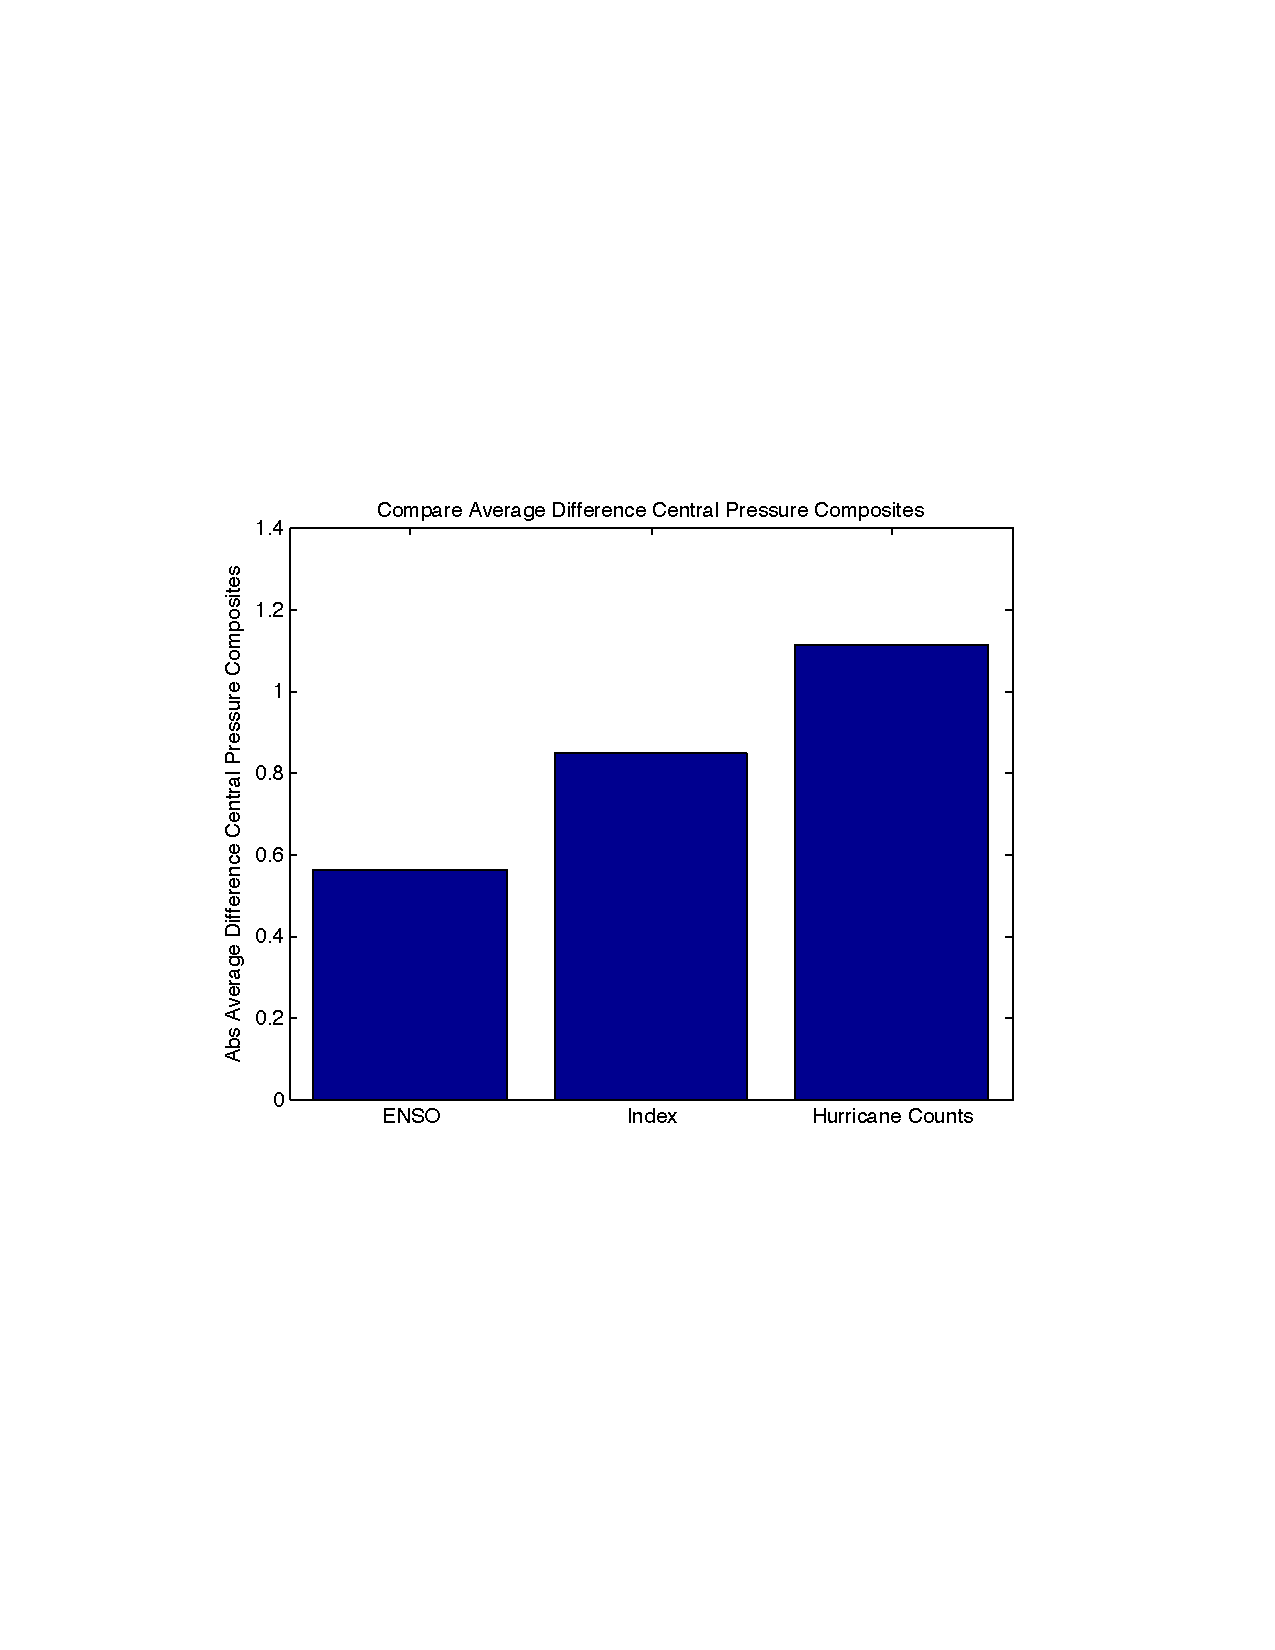
\includegraphics[width=\textwidth]{figs/sensitivityResults/compositeBarGraphs/centralPressureBarGraph.pdf}
\caption{Avg Diff Central Pressure}
\label{fig:figure29}
\end{minipage}
\hspace{0cm}
\begin{minipage}[b]{0.6\linewidth}
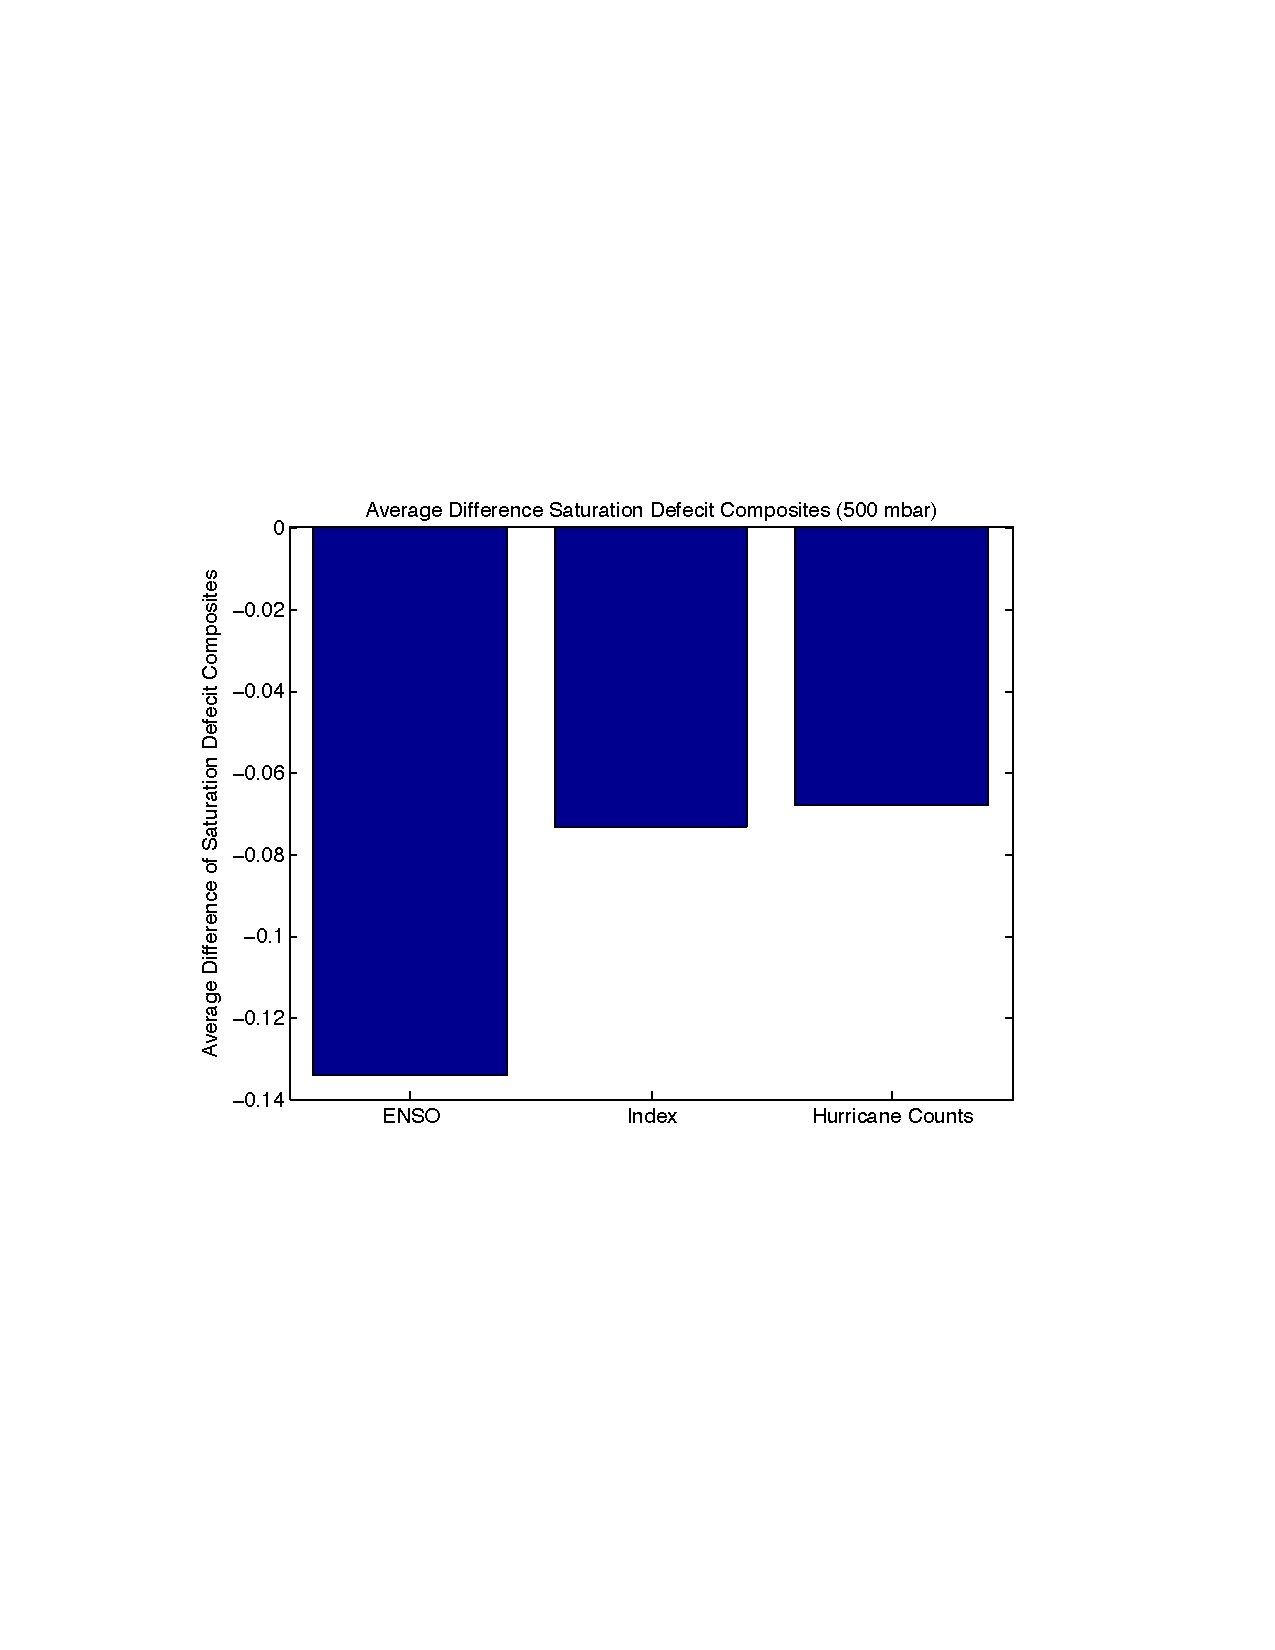
\includegraphics[width=\textwidth]{figs/sensitivityResults/compositeBarGraphs/satDefBarGraphSmallerBox.pdf}
\caption{Avg Diff Saturation Deficit}
\label{fig:figure30}
\end{minipage}
\end{figure}
\pagebreak
\begin{figure}[ht]
\begin{minipage}[b]{0.6\linewidth}
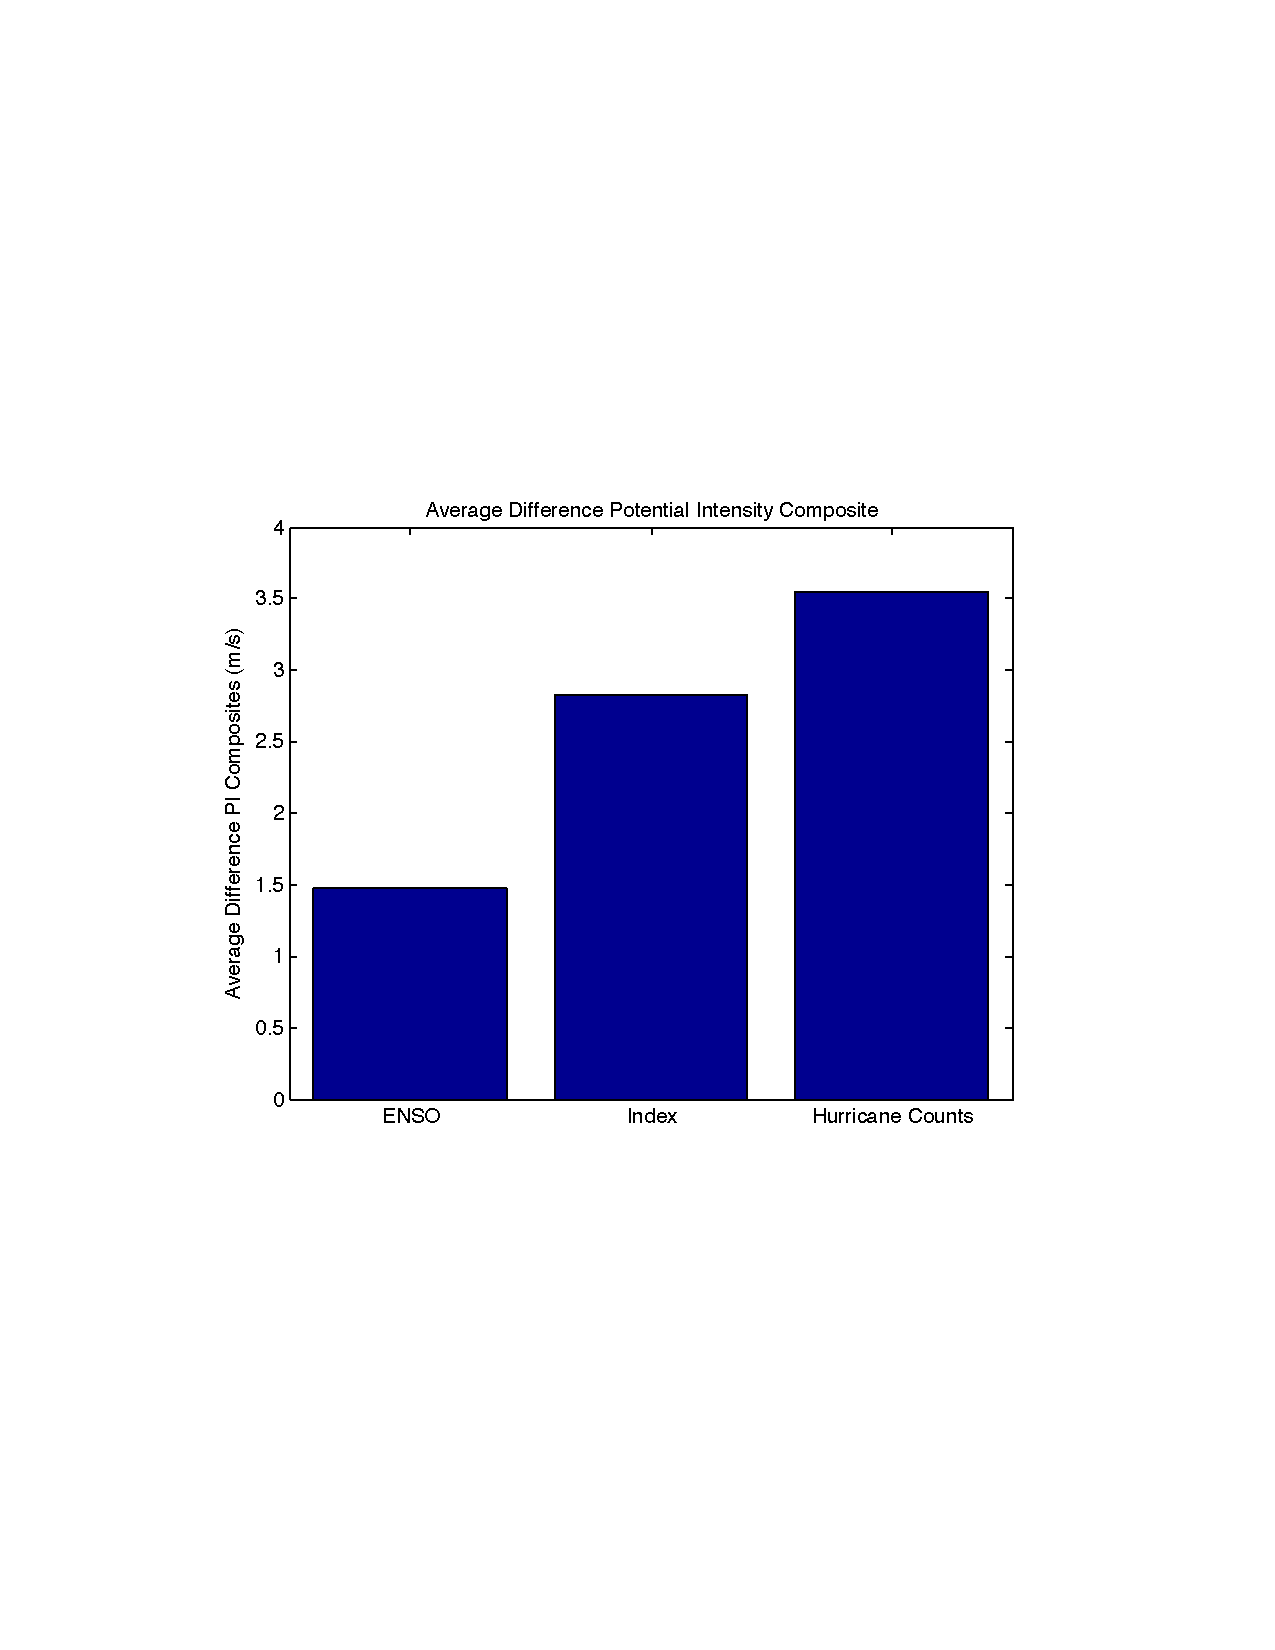
\includegraphics[width=\textwidth]{figs/sensitivityResults/compositeBarGraphs/avgDiffPIAtlanticCompositesBarGraph.pdf}
\caption{Avg Diff Potential Intensity}
\label{fig:figure31}
\end{minipage}
\hspace{0cm}
\begin{minipage}[b]{0.6\linewidth}
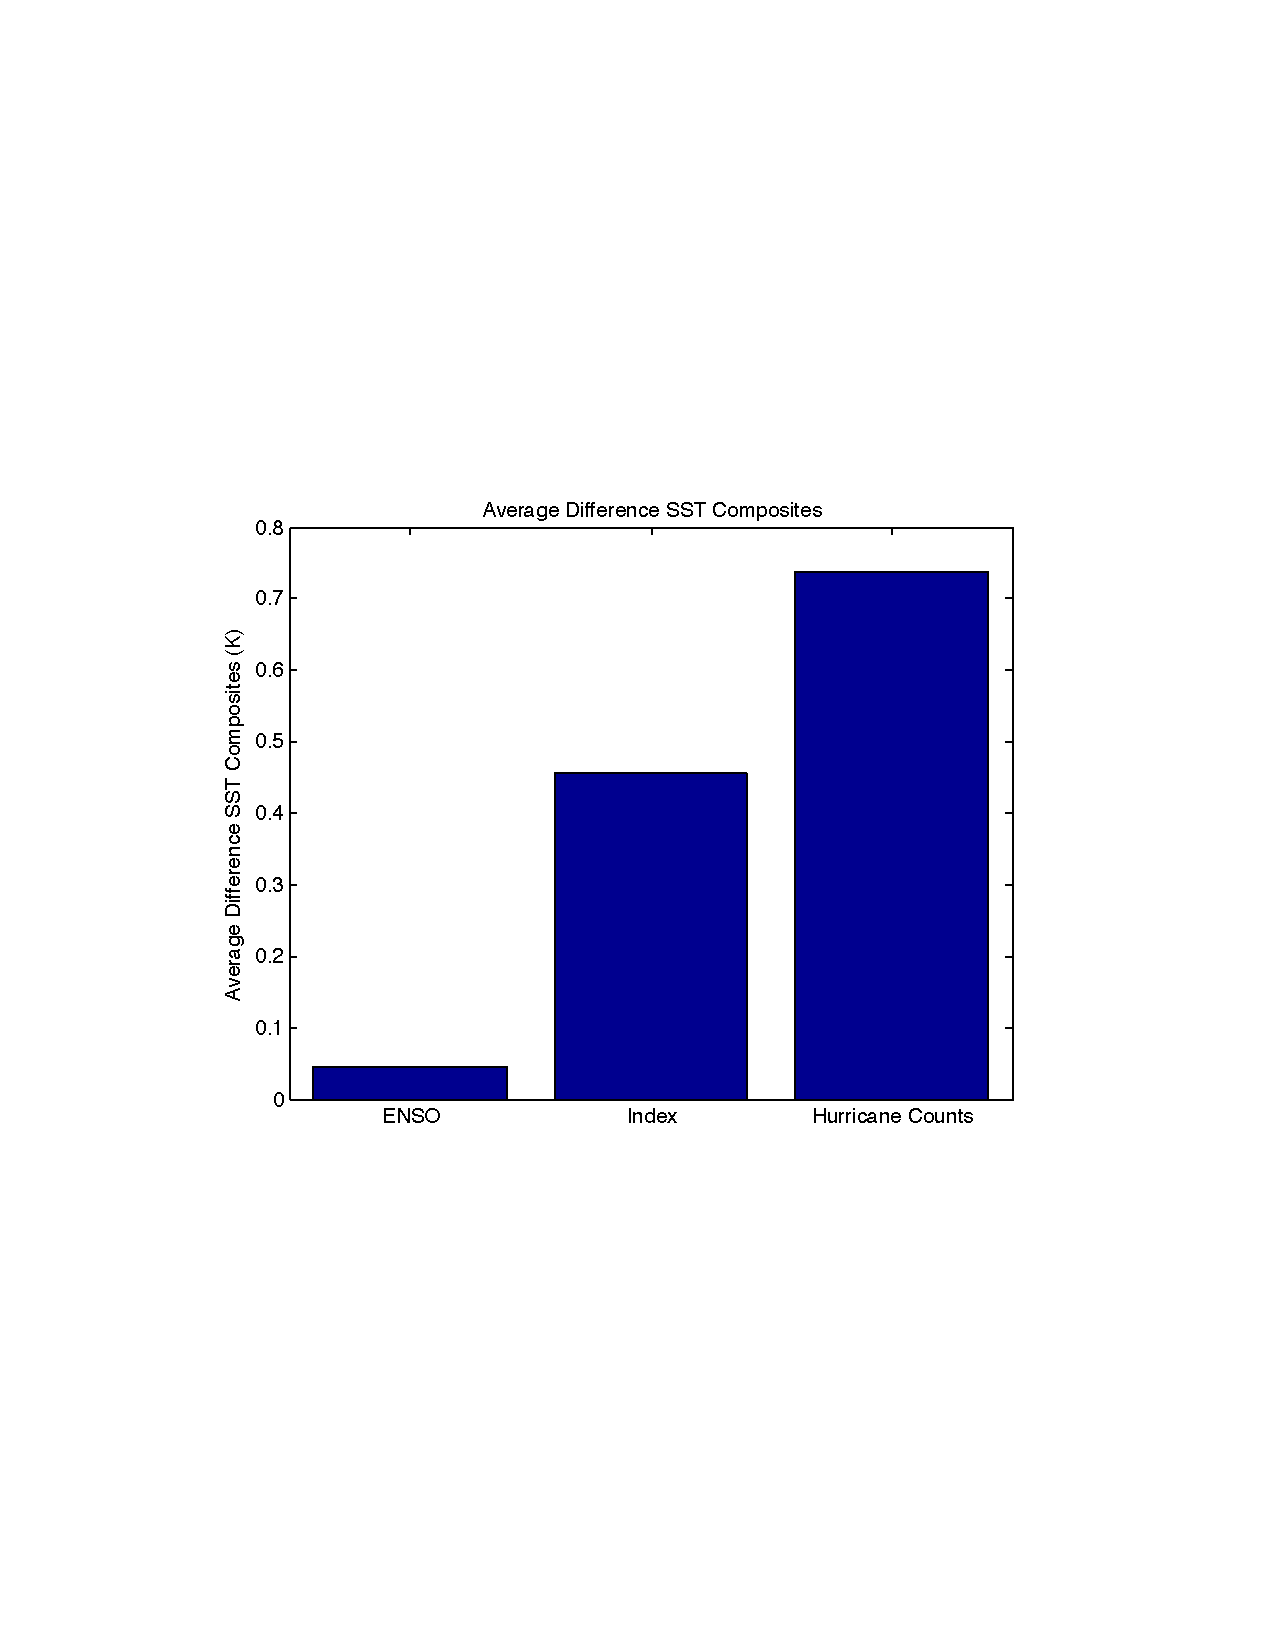
\includegraphics[width=\textwidth]{figs/sensitivityResults/compositeBarGraphs/sstBarGraph.pdf}
\caption{Avg Diff SST}
\label{fig:figure32}
\end{minipage}
\end{figure}

% Diedhiou \textit{et al.} \cite{diedhiou2010} looked at the large-scale conditions of 3 days leading to cyclogenesis off the West African coast. The potential of genesis is stronger before cyclogenesis over the West African coast than the climatology showing that strong low-level cyclonic vortices propagate from land to ocean in an atmosphere characterized by strong upper level support. Generally, before the occurrence of a cyclonic activity, the atmosphere is more unstable and African Easterly Waves are more active over West Africa than the climatology. Over the Atlantic Ocean, large scale conditions before cyclogenesis are characterized by the presence of high cyclogenesis contributors such as warmer waters, lower pressure, stronger mid-level humidity and higher degree of atmospheric instability.

%  \textit{Outgoing Longwave Radiation (OLR) data from NOAA (National Oceanic and Atmospheric Administration) are used to evaluate deep convection through low values (Grueber and Krueger, 1974).}
% \textit{The Potential of convection (PC) is a thermodynamic parameter used to study the degree of atmospheric instability. PC is the difference between the equivalent potential temperature at 1000 hPa (surface) and at 500 hPa (mid-troposphere): PC = $\theta_{1000} - \theta_{500}$ where $\theta$ is the equivalent to potential temperature.}
% The AEJ is a barotropic-baroclinic unstable jet in which develop AEWs that are the main precursors of Atlantic TCs (Burpee, 1972; Ross and Krishnamurti, 2007). These combined baroclinic – barotropic instabilities are studied using the meridional gradient of potential vorticity (PV) over isobaric levels according to Balasubramanian and Yau, (1996) who used the following formula -- see text.
 
% \section{MIC Analysis}
% \subsection{Pre-season - Cat 1-3}
% \begin{figure}[htbp]
% 	\centering
% 		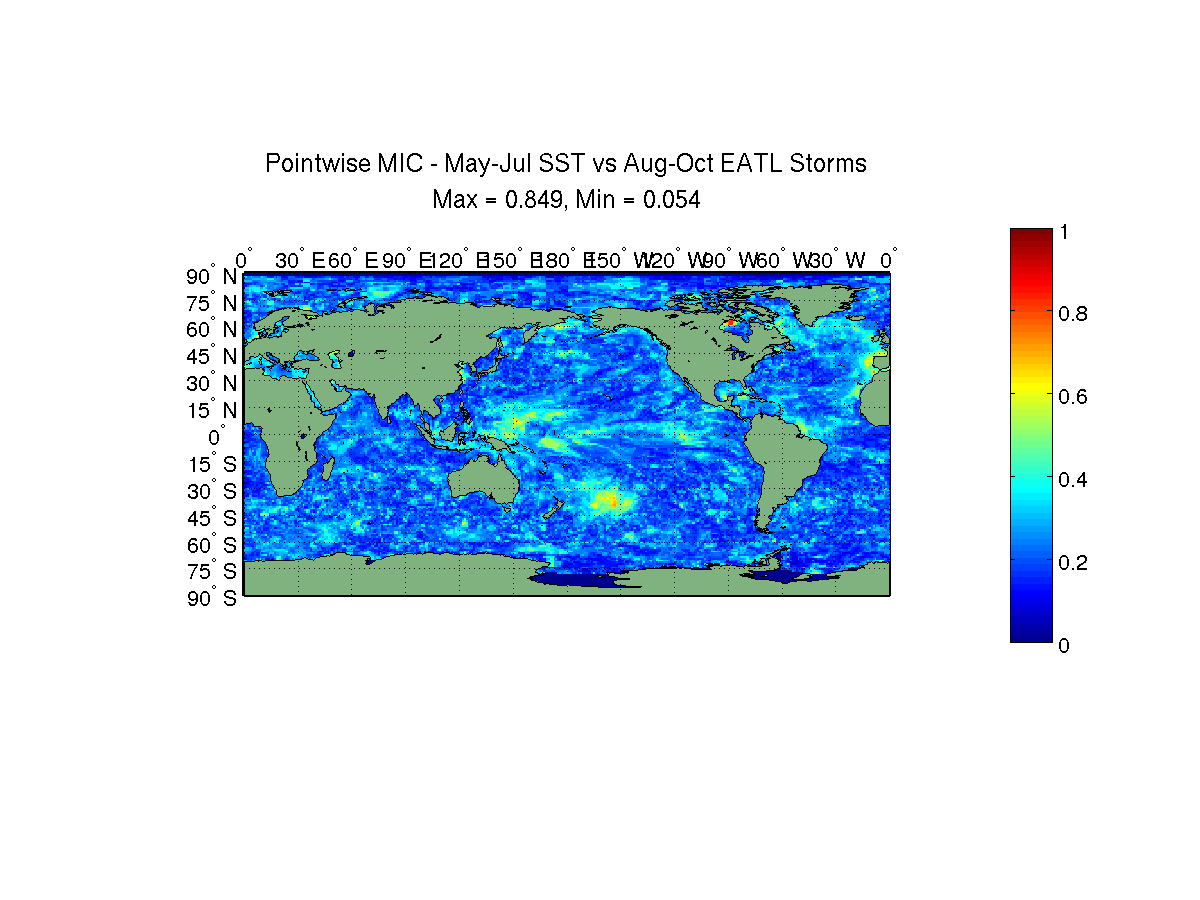
\includegraphics[height=3in]{figs/MICPointwiseCat1-3/EATLAug-Oct_May-Jul.png}
% 	\caption{Point-wise MIC score for May-July SST and ASO East Atlantic Cat1-3 Hurricanes. As in correlation analysis North Atlantic region and near Australia have high scores. \textbf{July only SST might be a better candidate}}
% 	\label{fig:figs_MICPointwiseCat1-3_EATLAug-Oct_May-Jul}
% \end{figure}
% \subsection{Pre-season - Cat 1-5}
% \begin{figure}[htbp]
% 	\centering
% 		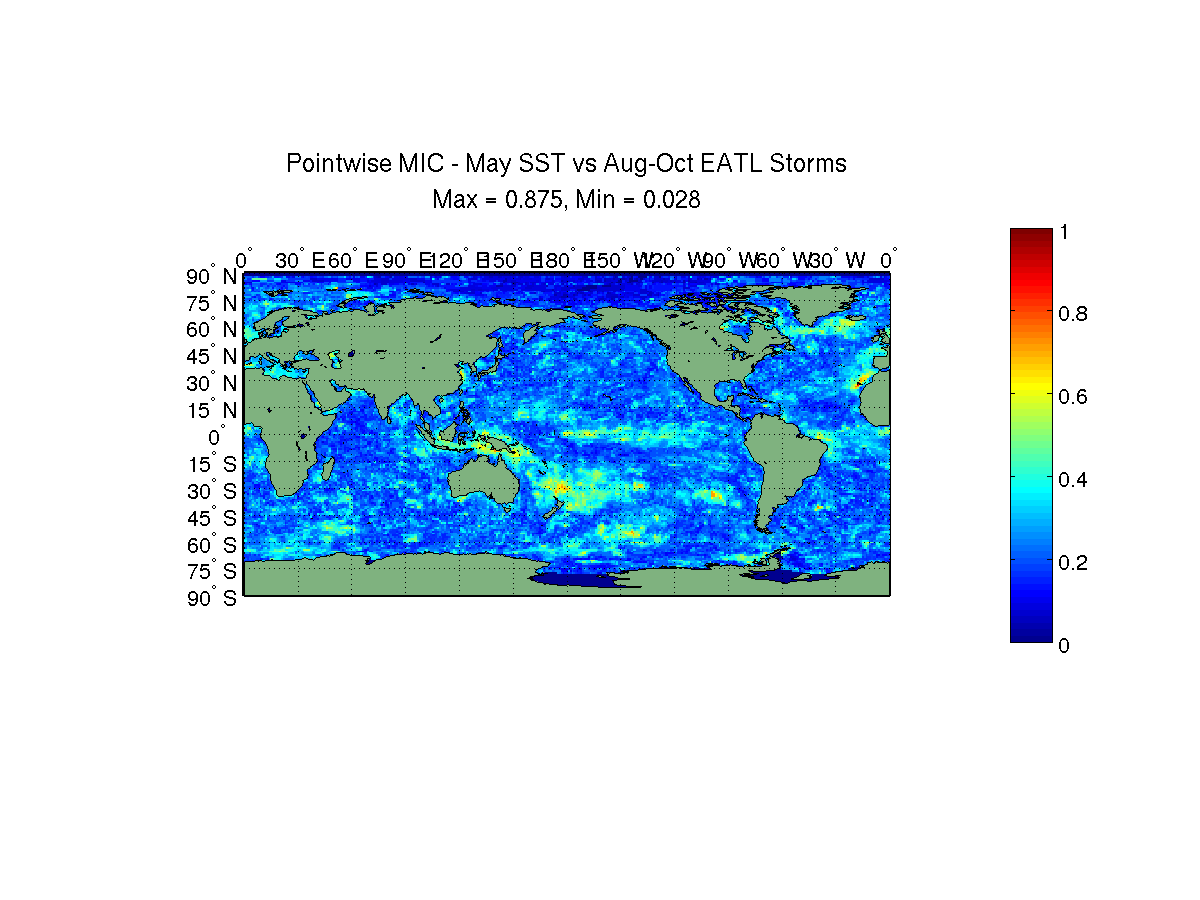
\includegraphics[height=3in]{figs/MICPointwiseCat1-5/EATLAug-Oct_May.png}
% 	\caption{May SST and ASO E. ATL Hurricanes (1-5)  }
% 	\label{fig:figs_MICPointwiseCat1-5_EATLAug-Oct_May}
% \end{figure}
% \begin{figure}[htbp]
% 	\centering
% 		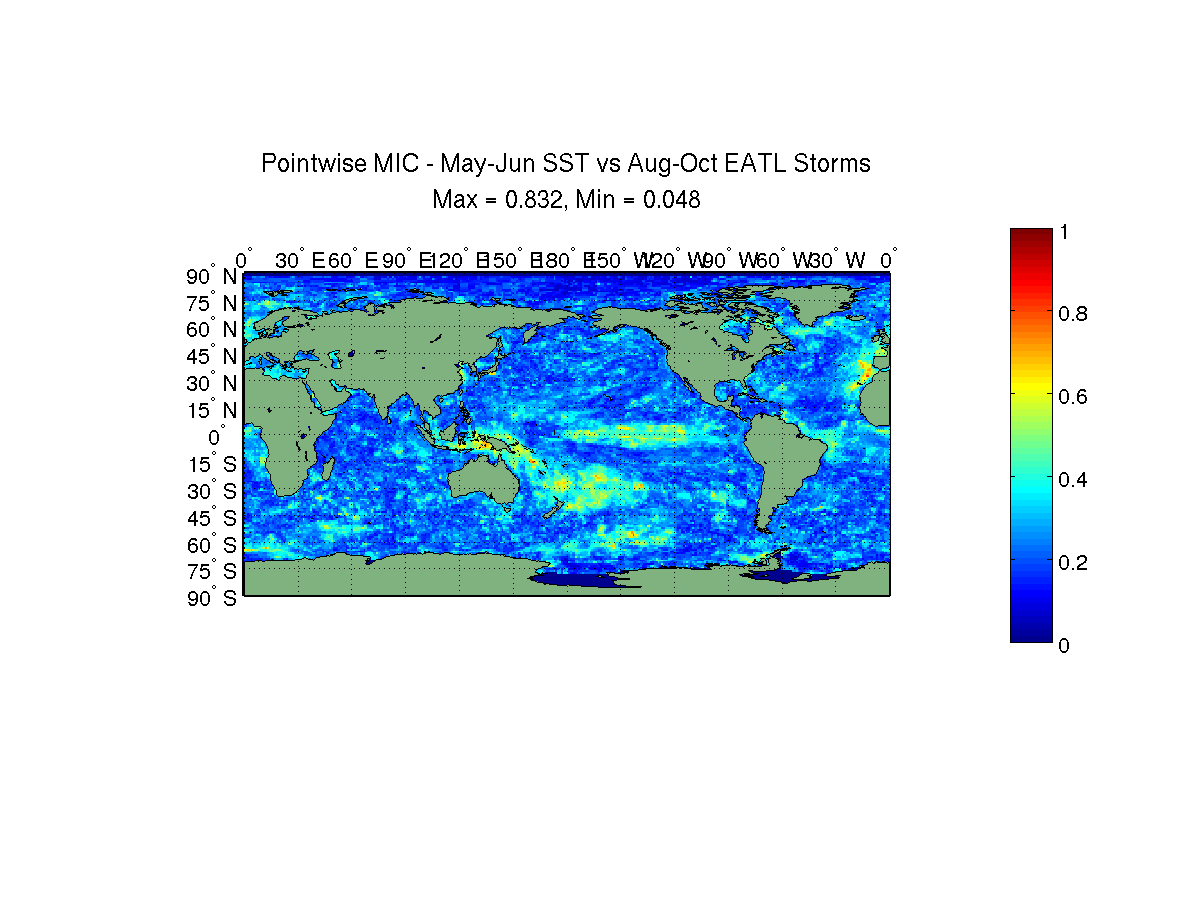
\includegraphics[height=3in]{figs/MICPointwiseCat1-5/EATLAug-Oct_May-Jun.png}
% 	\caption{May-June SST and ASO E. ATL Hurricanes (1-5)  }
% 	\label{fig:figs_MICPointwiseCat1-5_EATLAug-Oct_May-Jun}
% \end{figure}
% 
% \begin{figure}[htbp]
% 	\centering
% 		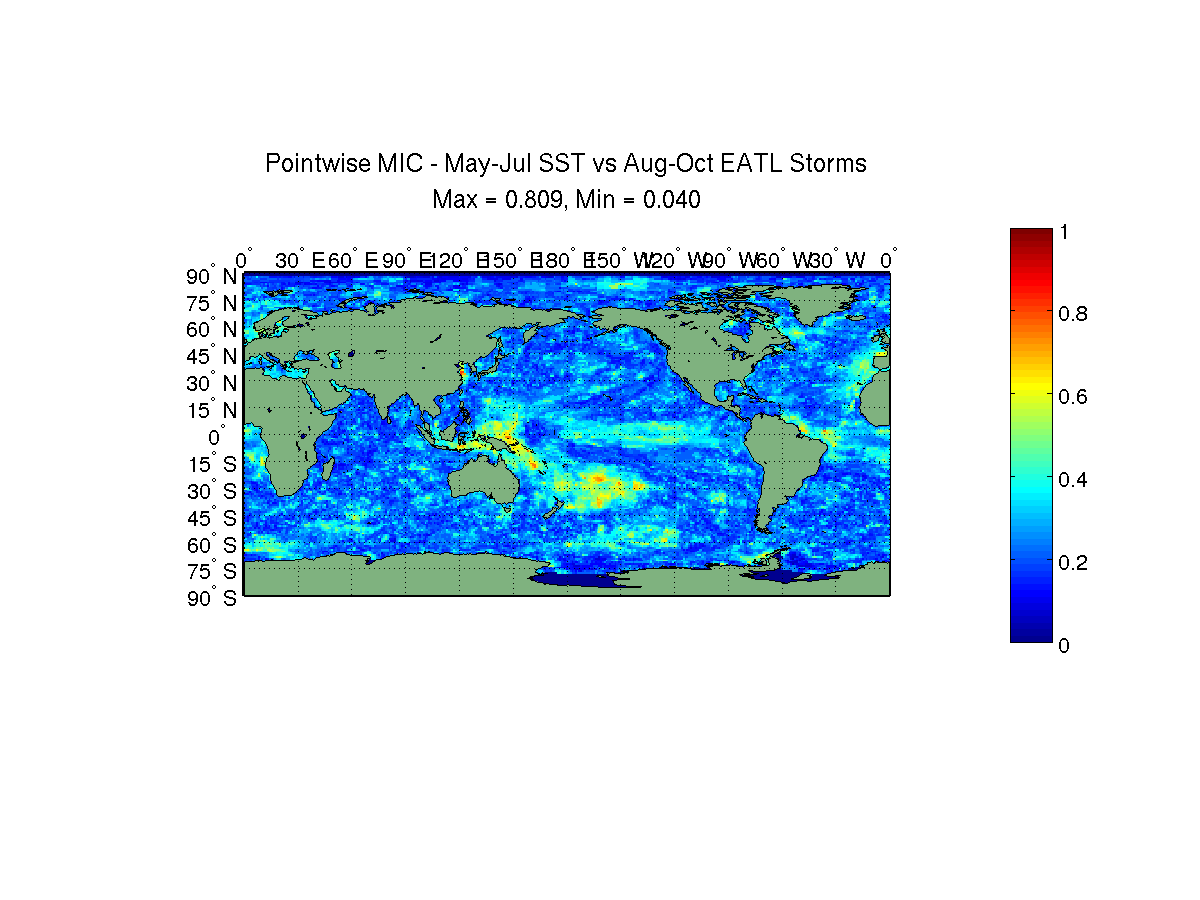
\includegraphics[height=3in]{figs/MICPointwiseCat1-5/EATLAug-Oct_May-Jul.png}
% 	\caption{May-July SST - ASO E. ATL Hurricanes (1-5)}
% 	\label{fig:figs_MICPointwiseCat1-5_EATLAug-Oct_May-Jul}
% \end{figure}
% 
% \begin{figure}[htbp]
% 	\centering
% 		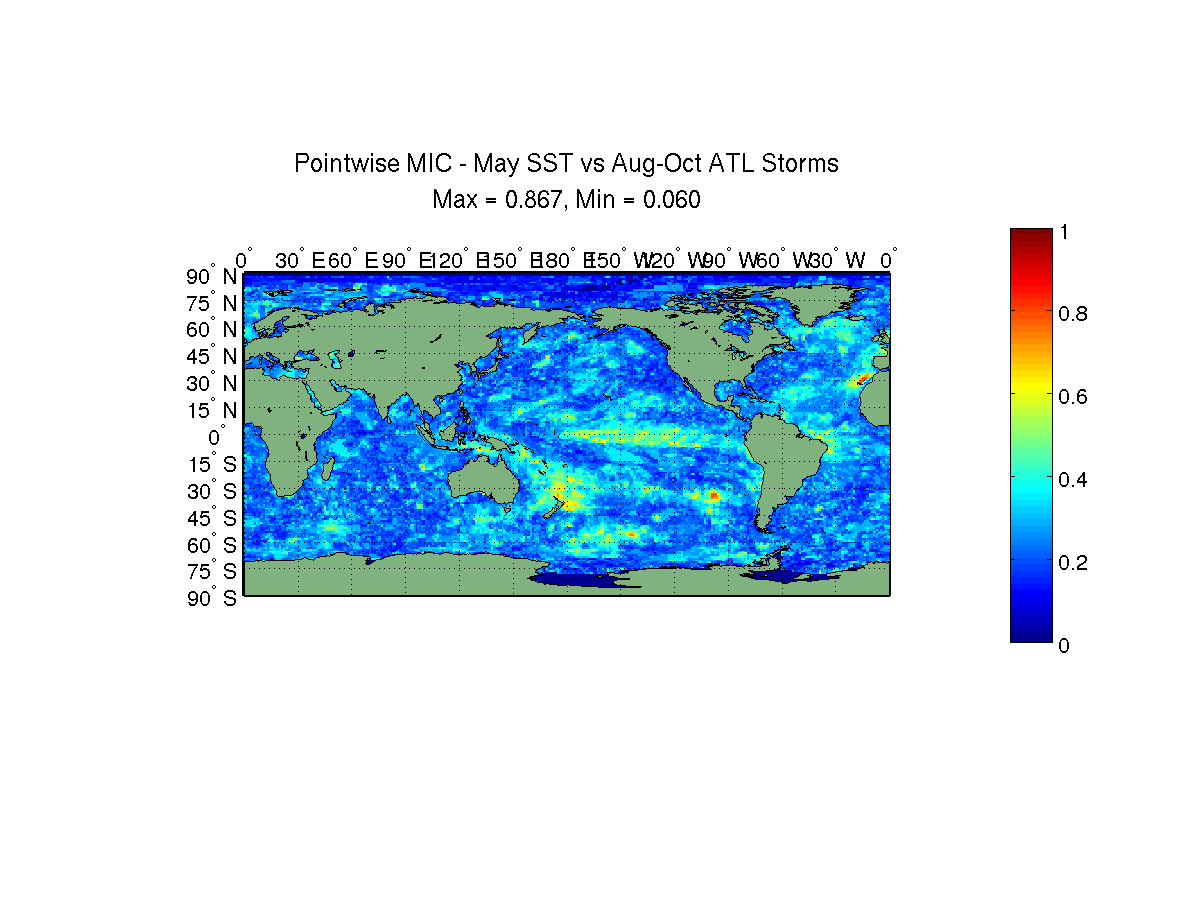
\includegraphics[height=3in]{figs/MICPointwiseCat1-5/ATLAug-Oct_May.png}
% 	\caption{May SST with MDR ASO Hurricanes}
% 	\label{fig:figs_MICPointwiseCat1-5_ATLAug-Oct_May}
% \end{figure}
% 
% \begin{figure}[htbp]
% 	\centering
% 		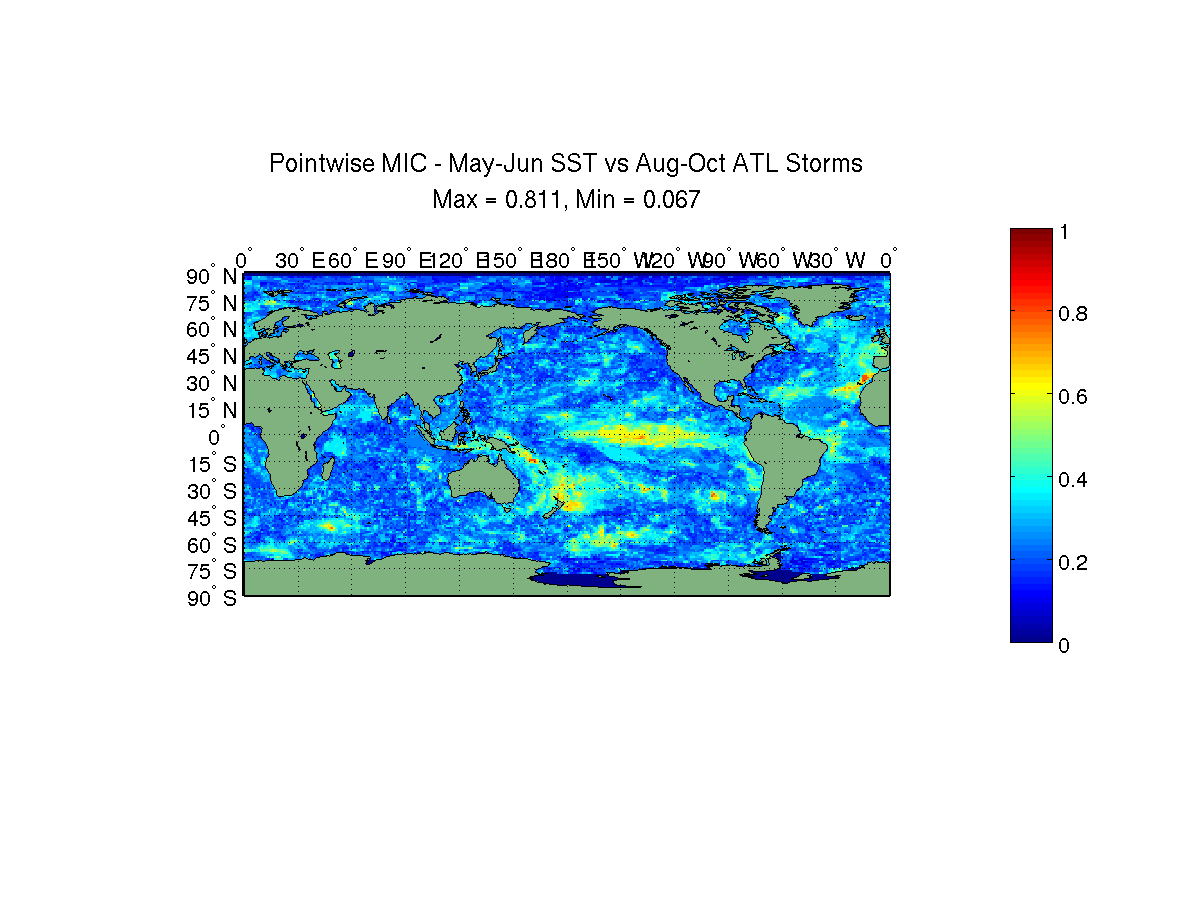
\includegraphics[height=3in]{figs/MICPointwiseCat1-5/ATLAug-Oct_May-Jun.png}
% 	\caption{May-June SST with MDR ASO Hurricanes}
% 	\label{fig:figs_MICPointwiseCat1-5_ATLAug-Oct_May-Jun}
% \end{figure}
% \begin{figure}[htbp]
% 	\centering
% 		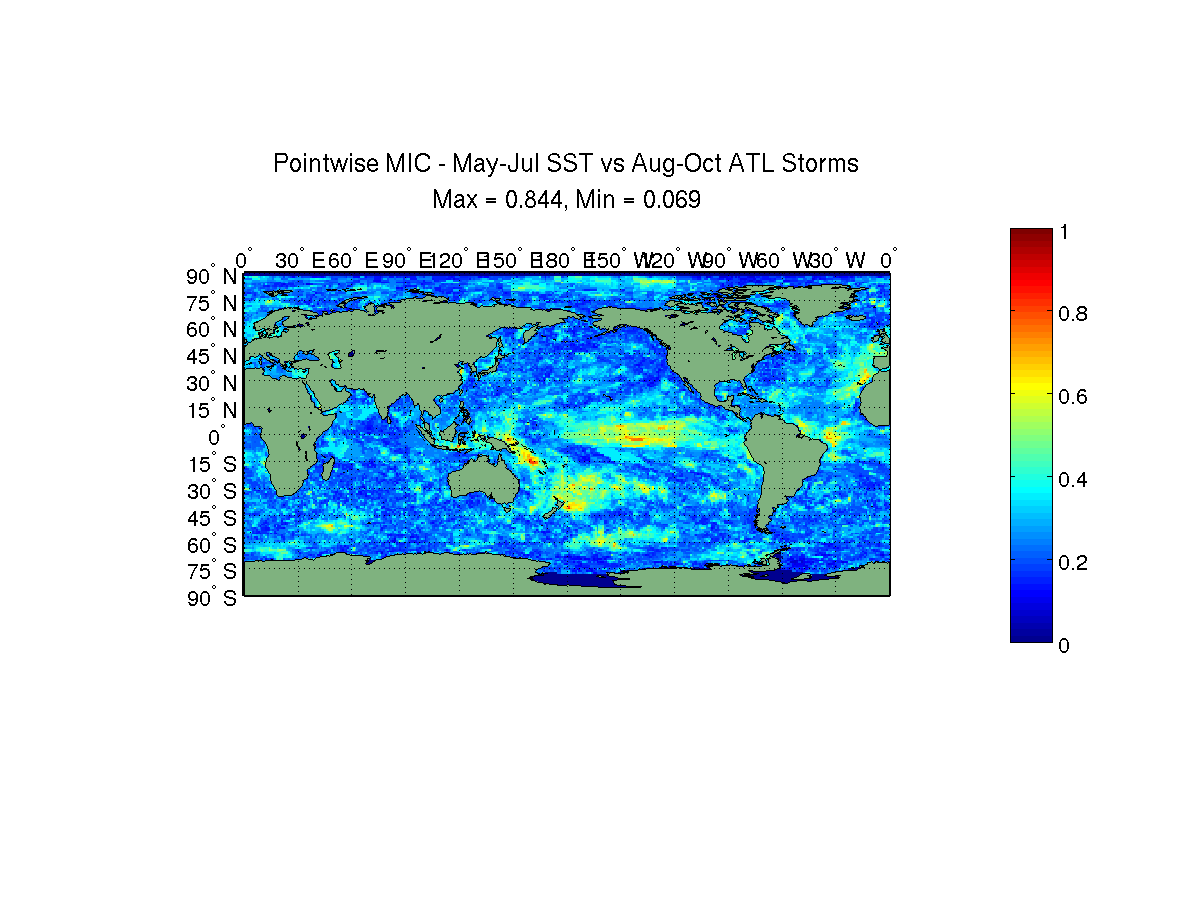
\includegraphics[height=3in]{figs/MICPointwiseCat1-5/ATLAug-Oct_May-Jul.png}
% 	\caption{May-July SST with MDR ASO Hurricanes}
% 	\label{fig:figs_MICPointwiseCat1-5_ATLAug-Oct_May-Jul}
% \end{figure}
% \subsection{Pre-Season Cat 4-5}
% \begin{figure}[htbp]
% 	\centering
% 		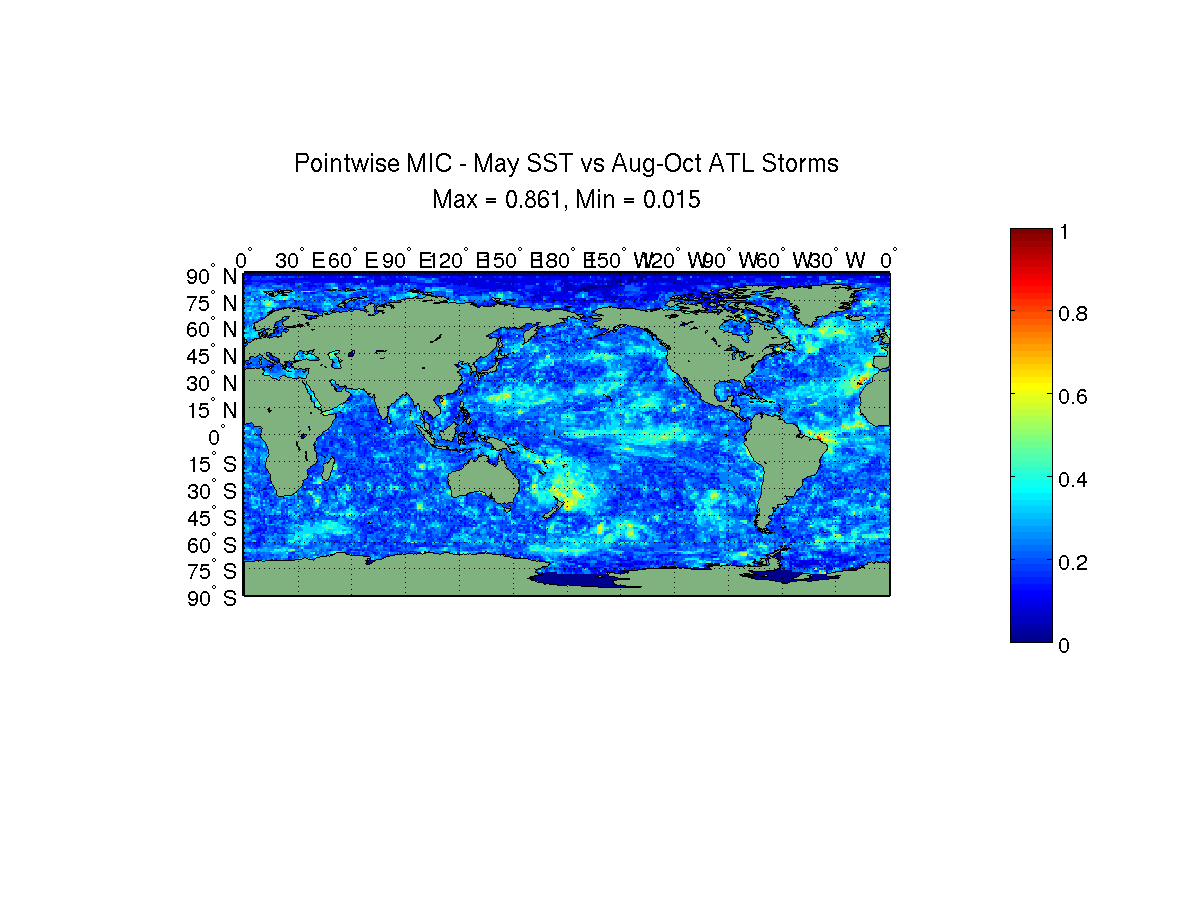
\includegraphics[height=3in]{figs/MICPointwiseCat4-5/ATLAug-Oct_May.png}
% 	\caption{May SST with MDR Cat4-5 Hurricanes ASO}
% 	\label{fig:figs_MICPointwiseCat4-5_ATLAug-Oct_May}
% \end{figure}
% 
% \begin{figure}[htbp]
% 	\centering
% 		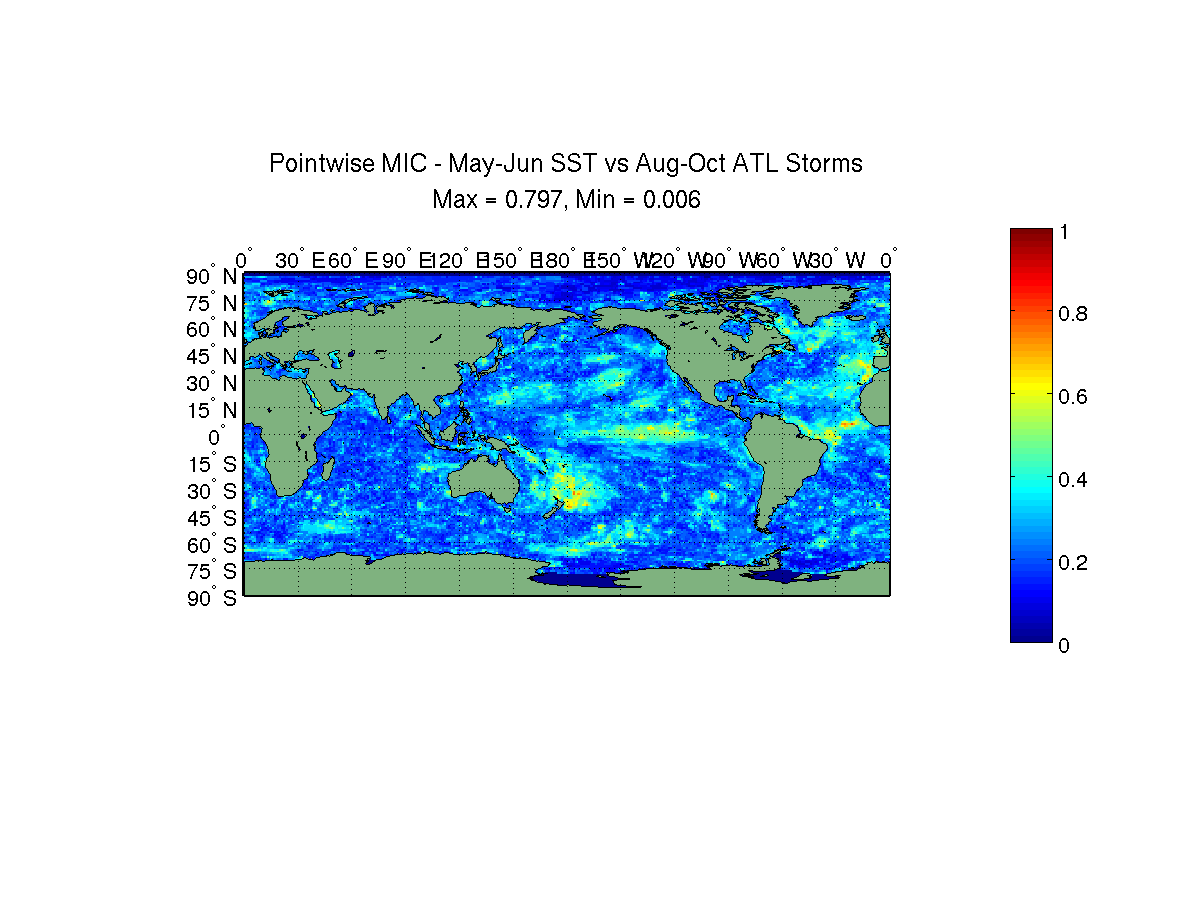
\includegraphics[height=3in]{figs/MICPointwiseCat4-5/ATLAug-Oct_May-Jun.png}
% 	\caption{May-June SST with MDR Cat4-5 Hurricanes ASO}
% 	\label{fig:figs_MICPointwiseCat4-5_ATLAug-Oct_May-Jun}
% \end{figure}
% \begin{figure}[htbp]
% 	\centering
% 		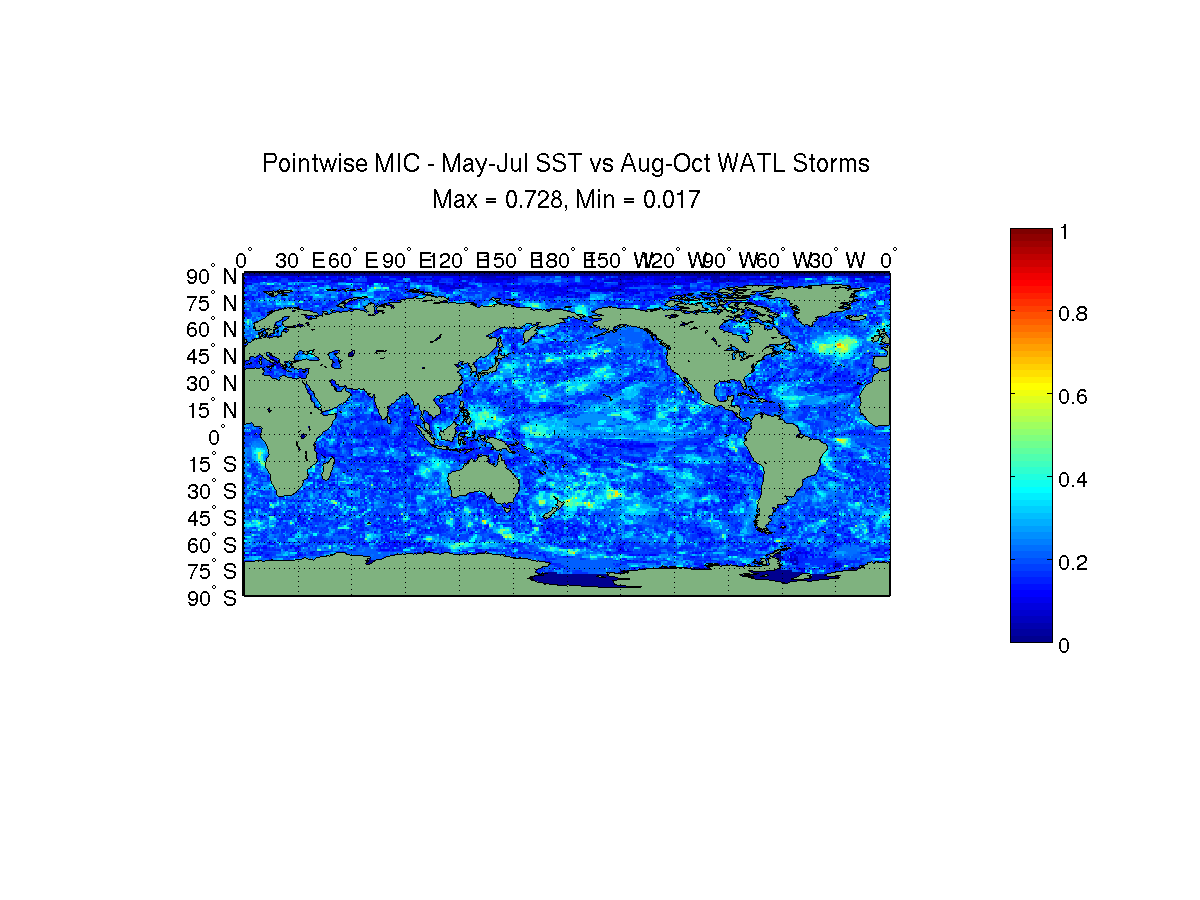
\includegraphics[height=3in]{figs/MICPointwiseCat4-5/WATLAug-Oct_May-Jul.png}
% 	\caption{May-July SST and W. ATL Cat 4-5 Hurricanes ASO}
% 	\label{fig:figs_MICPointwiseCat4-5_WATLAug-Oct_May-Jul}
% \end{figure}
% 
% \subsection{TCs with SST from 1971}
%  
% \begin{figure}[htbp]
% 	\centering
% 		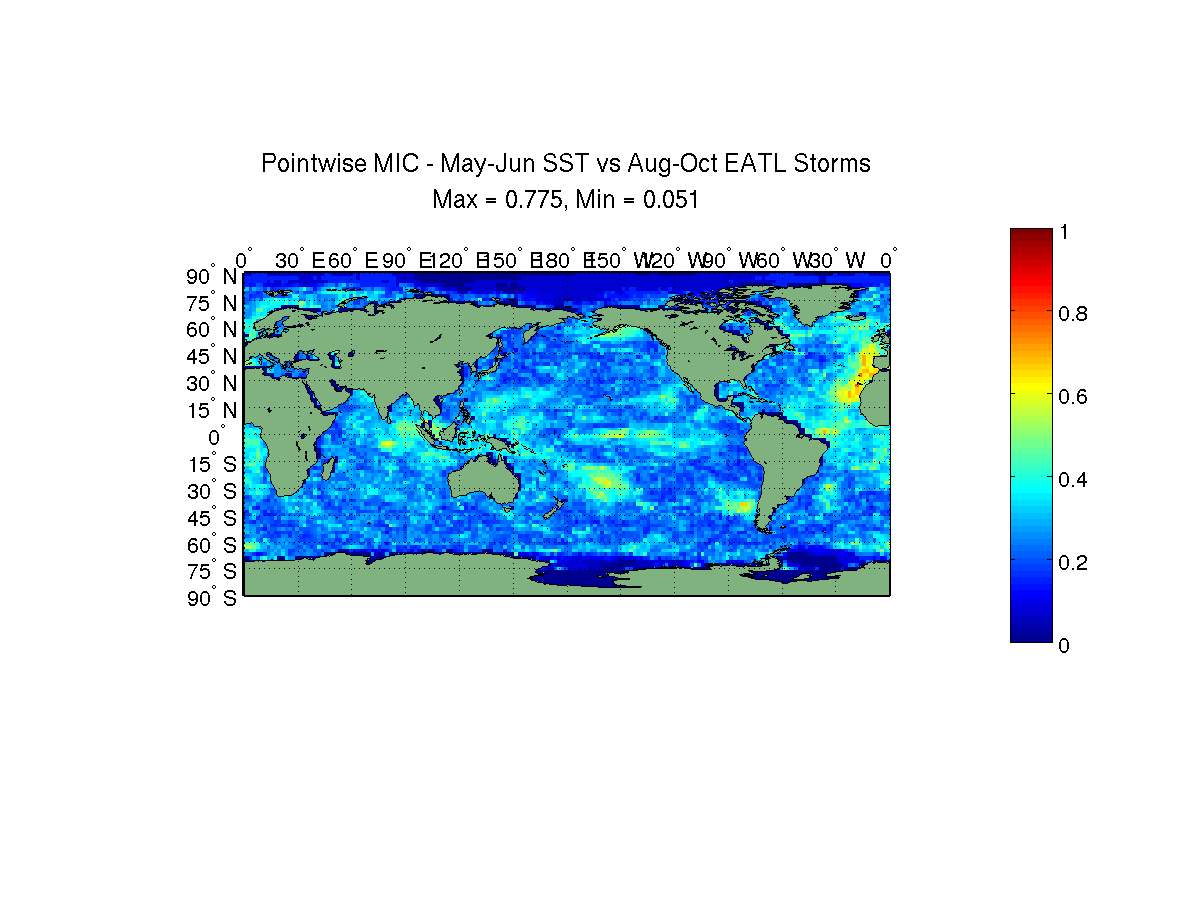
\includegraphics[height=5in]{figs/MICPointwiseExtended/EATLAug-Oct_May-Jun.png}
% 	\caption{May-June SST - ASO TCs 1971-2010}
% 	\label{fig:figs_MICPointwiseExtended_EATLAug-Oct_May-Jun}
% \end{figure}
% 
% \begin{figure}[htbp]
% 	\centering
% 		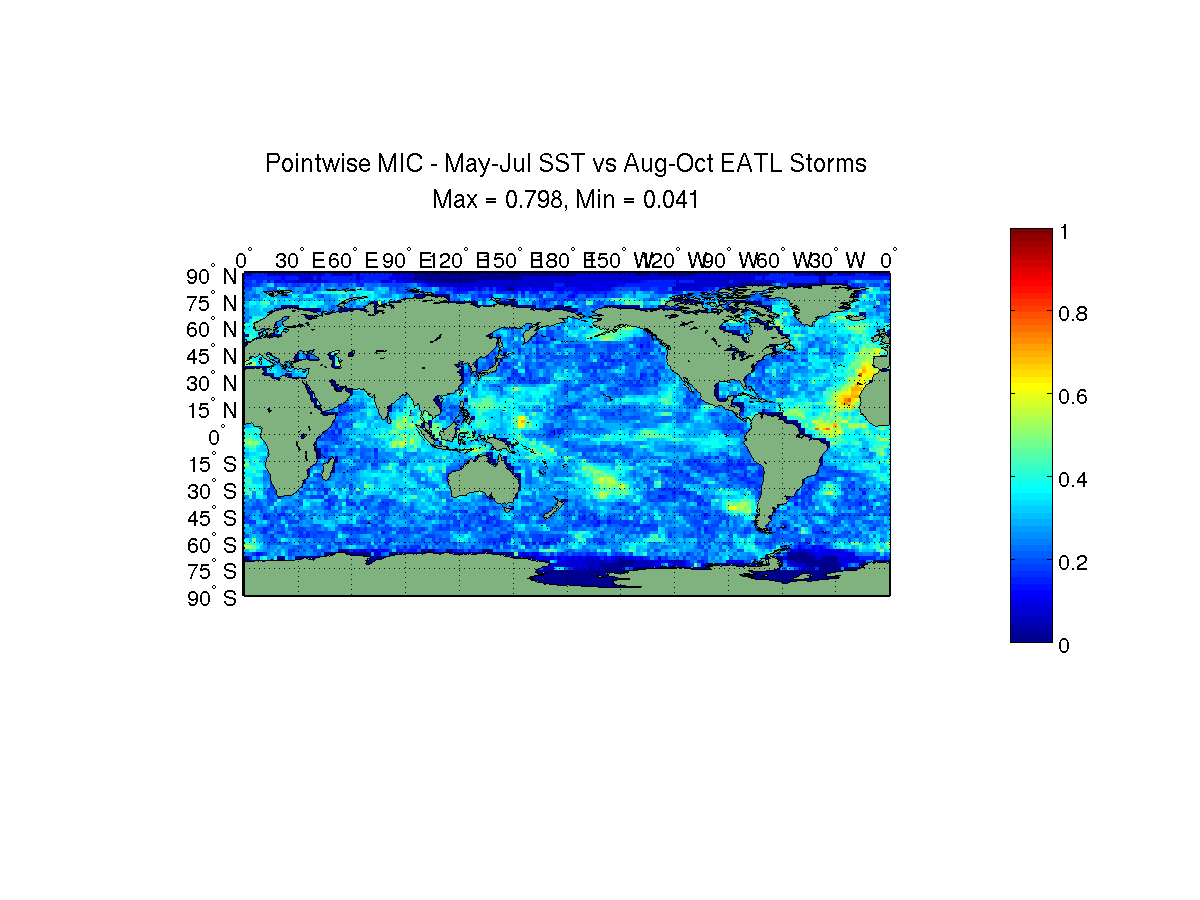
\includegraphics[height=5in]{figs/MICPointwiseExtended/EATLAug-Oct_May-Jul.png}
% 	\caption{May-July SST - ASO TCs 1971-2010}
% 	\label{fig:figs_MICPointwiseExtended_EATLAug-Oct_May-Jul}
% \end{figure}
% 
% \subsection{MIC Vs. CC}
% \begin{figure}[htbp]
% 	\centering
% 		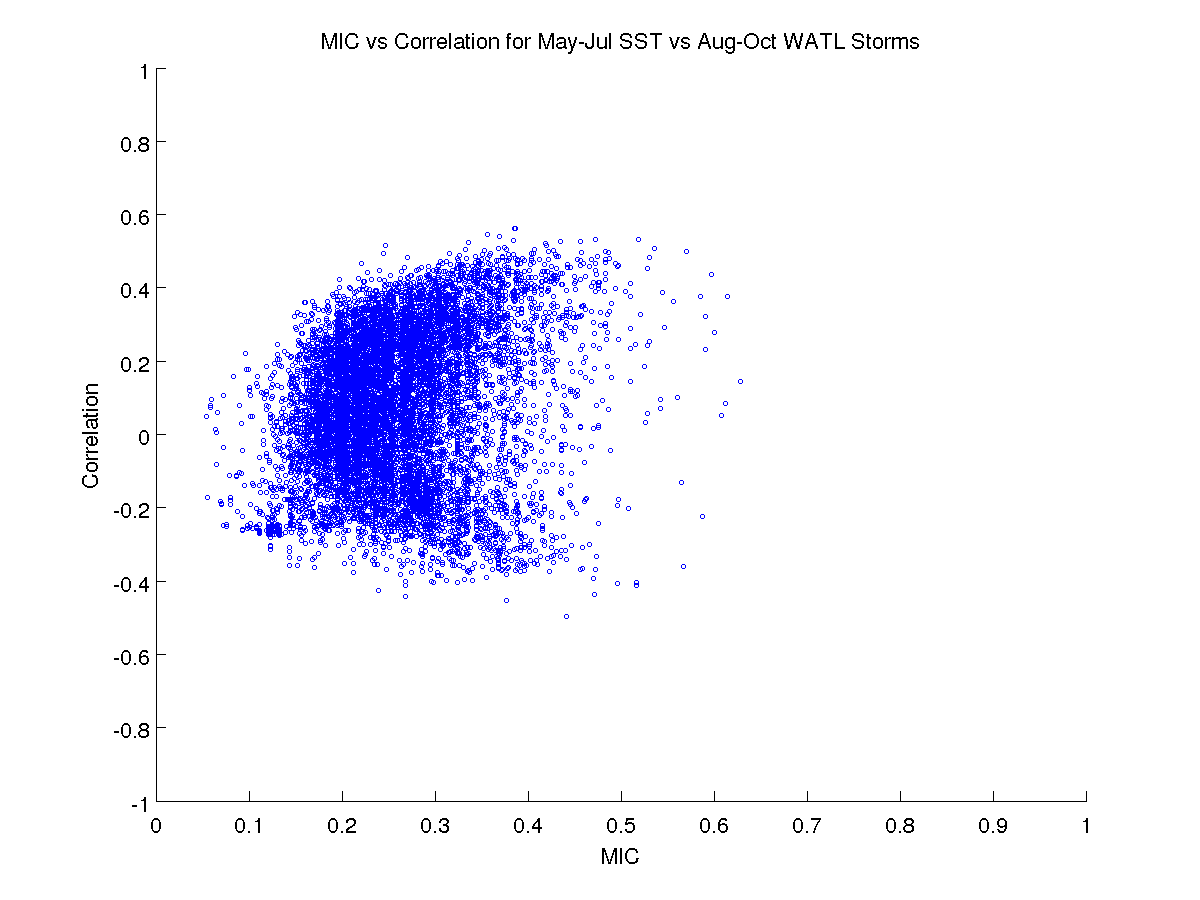
\includegraphics[height=3in]{figs/MICPointwiseExtended/WATLAug-Oct_May-Jul_CCvsMIC.png}
% 	\caption{MIC and CC for May-Jul SST and ASO W. ATL TCs 1971-2010}
% 	\label{fig:figs_MICPointwiseExtended_WATLAug-Oct_May-Jul_CCvsMIC}
% \end{figure}
% \begin{figure}[htbp]
% 	\centering
% 		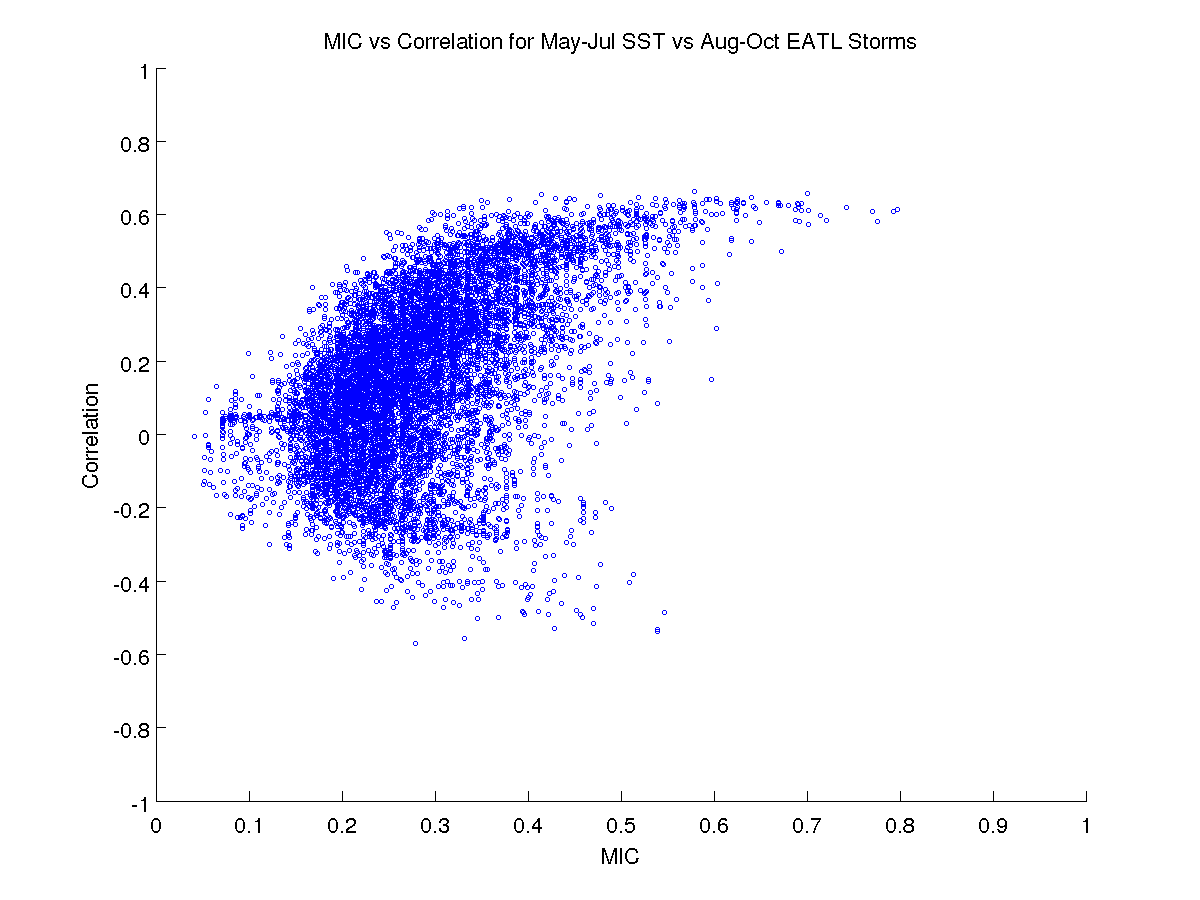
\includegraphics[height=3in]{figs/MICPointwiseExtended/EATLAug-Oct_May-Jul_CCvsMIC.png}
% 	\caption{MIC and CC for May-Jul SST and ASO E. ATL TCs 1971-2010}
% 	\label{fig:figs_MICPointwiseExtended_EATLAug-Oct_May-Jul_CCvsMIC}
% \end{figure}
% \begin{figure}[htbp]
% 	\centering
% 		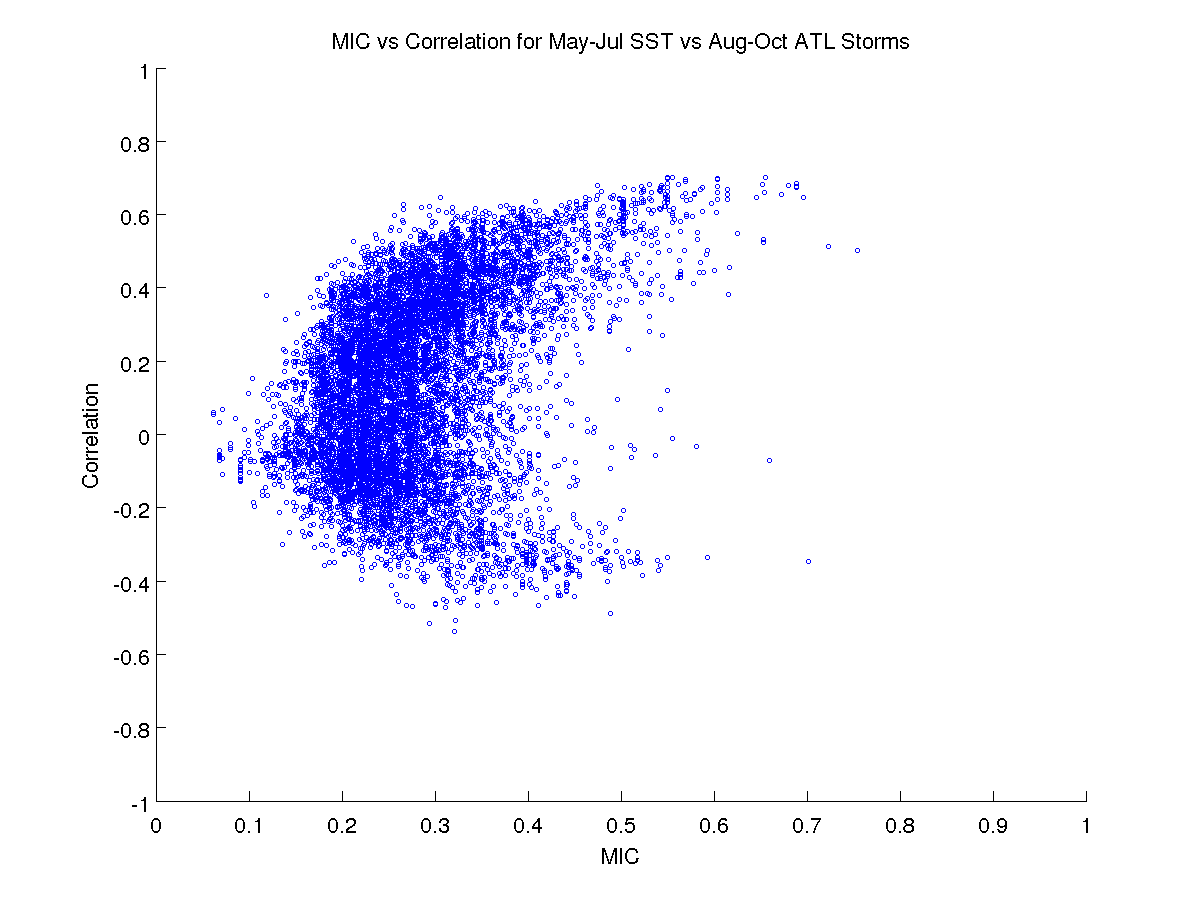
\includegraphics[height=3in]{figs/MICPointwiseExtended/ATLAug-Oct_May-Jul_CCvsMIC.png}
% 	\caption{MIC and CC for May-Jul SST and ASO MDR TCs 1971-2010}
% 	\label{fig:figs_MICPointwiseExtended_ATLAug-Oct_May-Jul_CCvsMIC}
% \end{figure}


\bibliographystyle{plain}
\bibliography{hurricanes_copy}
 
\end{document}
